\documentclass[11pt,a4paper]{article}

% ========================================
% PACKAGES
% ========================================
\usepackage[utf8]{inputenc}
\usepackage[T1]{fontenc}
\usepackage{lmodern}  % Better font support for larger sizes
\usepackage[english]{babel}  % Change to your language
\usepackage[margin=2.5cm]{geometry}

% Mathematics
\usepackage{amsmath, amssymb, amsthm}
\usepackage{mathtools}

% Graphics and colors
\usepackage{graphicx}
\usepackage{xcolor}
\usepackage{tikz}
\usetikzlibrary{positioning, arrows.meta, shapes.geometric, calc}
\usepackage{pgfplots}
\pgfplotsset{compat=1.18}
\usepackage[most]{tcolorbox}

% Lists and formatting
\usepackage{enumitem}
\usepackage{parskip}
\usepackage{fancyhdr}

% Code listings (if needed)
\usepackage{listings}
\usepackage{algorithm}
\usepackage{algorithmic}

% Hyperlinks
\usepackage{hyperref}
\hypersetup{
    colorlinks=true,
    linkcolor=blue,
    urlcolor=blue,
    citecolor=blue
}

% ========================================
% THEOREM ENVIRONMENTS
% ========================================
\theoremstyle{definition}
\newtheorem{definition}{Definition}[section]
\newtheorem{example}{Example}[section]
\newtheorem{exercise}{Exercise}[section]

\theoremstyle{plain}
\newtheorem{theorem}{Theorem}[section]
\newtheorem{lemma}[theorem]{Lemma}
\newtheorem{proposition}[theorem]{Proposition}
\newtheorem{corollary}[theorem]{Corollary}

\theoremstyle{remark}
\newtheorem*{remark}{Remark}
\newtheorem*{observation}{Observation}

% ========================================
% CUSTOM COMMANDS
% ========================================
\newcommand{\R}{\mathbb{R}}
\newcommand{\N}{\mathbb{N}}
\newcommand{\Z}{\mathbb{Z}}
\newcommand{\Q}{\mathbb{Q}}
\newcommand{\C}{\mathbb{C}}

% ========================================
% TABLE OF CONTENTS DEPTH
% ========================================
\setcounter{tocdepth}{2} % Show only parts, sections, and subsections

% ========================================
% HEADER AND FOOTER
% ========================================
\setlength{\headheight}{14pt}
\pagestyle{fancy}
\fancyhf{}
\lhead{\leftmark}
\rhead{DL}
\cfoot{\thepage}
\renewcommand{\sectionmark}[1]{\markboth{#1}{}}

% ========================================
% DOCUMENT INFORMATION
% ========================================
\title{\textbf{Deep Learning}\\
\large Artificial Intelligence}
\author{Jacopo Parretti}
\date{II Semester 2025-2026}

% ========================================
% DOCUMENT
% ========================================
\begin{document}

\maketitle
\tableofcontents
\newpage


% ========================================
\part{Introduction to Deep Learning}
% ========================================

\section{What is Deep Learning?}

\subsection{Positioning within AI}

\textbf{Deep Learning} is a subset of machine learning and, more specifically, of \textbf{representation learning} (also called \textit{feature learning}). The fundamental goal is to \emph{learn underlying features directly from data}, eliminating the need for hand-engineered feature extractors.

The standard machine learning pipeline separates two concerns: \textbf{feature extraction}, designed by a domain expert, and \textbf{classification}, learned from labeled examples. Deep learning collapses this pipeline --- the network performs both steps jointly, learning task-relevant representations end-to-end from raw input.

\begin{figure}[h]
    \centering
    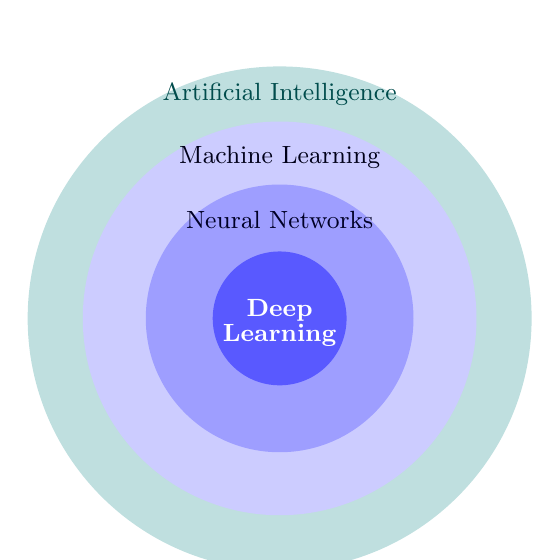
\begin{tikzpicture}
        \foreach \r/\col in {3.2/teal!25, 2.5/blue!20, 1.7/blue!38, 0.85/blue!65} {
            \fill[\col] (0,0) circle (\r);
        }
        \node[white, font=\bfseries\small] at (0, 0.1)   {Deep};
        \node[white, font=\bfseries\small] at (0, -0.22) {Learning};
        \node[blue!15!black, font=\small]  at (0, 1.25)  {Neural Networks};
        \node[blue!10!black, font=\small]  at (0, 2.05)  {Machine Learning};
        \node[teal!60!black, font=\small]  at (0, 2.85)  {Artificial Intelligence};
    \end{tikzpicture}
    \caption{Deep Learning as a nested subset of AI.}\label{fig:dl-subset}
\end{figure}

\subsection{Why Deep Learning?}

A critical empirical observation motivates deep learning: as the volume of available data grows, most classical learning algorithms \textbf{plateau} in performance, while deep neural networks \textbf{continue to improve}. This favorable scaling behavior, combined with large-scale datasets and modern hardware accelerators, explains the field's current dominance.

\subsection{Deep Learning as Representation Learning}

Deep learning is explicitly a form of \textbf{representation learning}: the network learns a hierarchy of representations, layer by layer, from raw input to task-relevant abstractions. In visual recognition, the hierarchy proceeds roughly as:

\begin{itemize}
    \item \textbf{Visible layer}: raw pixel values
    \item \textbf{1st hidden layer}: low-level features (edges, color blobs)
    \item \textbf{2nd hidden layer}: mid-level features (corners, contours)
    \item \textbf{3rd hidden layer}: high-level features (object parts)
    \item \textbf{Output layer}: class identity (car, person, animal, \ldots)
\end{itemize}

The deeper the network, the more abstract and task-specific the learned representations.

\subsection{Why Representation Matters}

The choice of representation fundamentally affects the difficulty of learning. A canonical example: two point clouds that cannot be separated by a linear boundary in Cartesian coordinates $(x, y)$ become trivially linearly separable after converting to polar coordinates $(r, \theta)$. Deep networks learn such transformations automatically, avoiding the need for manual feature engineering.


\section{A Brief History of Neural Networks}

The current success of deep learning is recent, but its intellectual roots extend to the 1940s. Three factors explain the modern renaissance:

\begin{enumerate}
    \item \textbf{Big data}: availability of massive labeled datasets (e.g., ImageNet, web-scale corpora).
    \item \textbf{Improved software}: modern frameworks (PyTorch, TensorFlow) with automatic differentiation and GPU support.
    \item \textbf{Hardware}: GPUs and TPUs provide the parallelism required to train large models in tractable time.
\end{enumerate}

Key milestones (1943--present):

\begin{itemize}
    \item \textbf{1943}: McCulloch \& Pitts model a neuron with electrical circuits.
    \item \textbf{1949}: Hebb formalizes synaptic plasticity in \textit{The Organization of Behavior}.
    \item \textbf{1956}: The Dartmouth Summer Research Project launches AI as a field.
    \item \textbf{1957--58}: Rosenblatt develops the \textbf{Perceptron} --- the oldest neural network still in common use today.
    \item \textbf{1959}: Widrow \& Hoff develop ADALINE and MADALINE --- the first neural network applied to a real-world problem.
    \item \textbf{1969}: Minsky \& Papert prove the Perceptron's fundamental limitations (\textit{Perceptrons}); neural network research stalls.
    \item \textbf{1981--82}: Hopfield presents energy-based associative memory; interest revives.
    \item \textbf{1985}: Backpropagation popularized (Rumelhart, Hinton, Williams).
    \item \textbf{1997}: LSTM proposed by Schmidhuber \& Hochreiter.
    \item \textbf{1998}: LeCun publishes \textit{Gradient-Based Learning Applied to Document Recognition}.
    \item \textbf{Now}: neural networks are ubiquitous; discussions about their future are prevalent.
\end{itemize}


\section{The Perceptron}

The \textbf{perceptron} is the basic building block of neural networks, introduced by Frank Rosenblatt in 1958. It is a computational abstraction of a biological neuron.

\begin{definition}[Perceptron]
A perceptron takes $m$ real-valued inputs $x_1, \ldots, x_m$ together with a constant bias $w_0$, computes their weighted sum, and passes the result through an activation function $g$:
\[
    \hat{y} = g\!\left(w_0 + \sum_{i=1}^{m} x_i\, w_i\right)
\]
In the original formulation, $g$ is the Heaviside step function. Information flows strictly \textbf{forward}: from inputs to output, with no feedback connections.
\end{definition}

\begin{figure}[h]
    \centering
    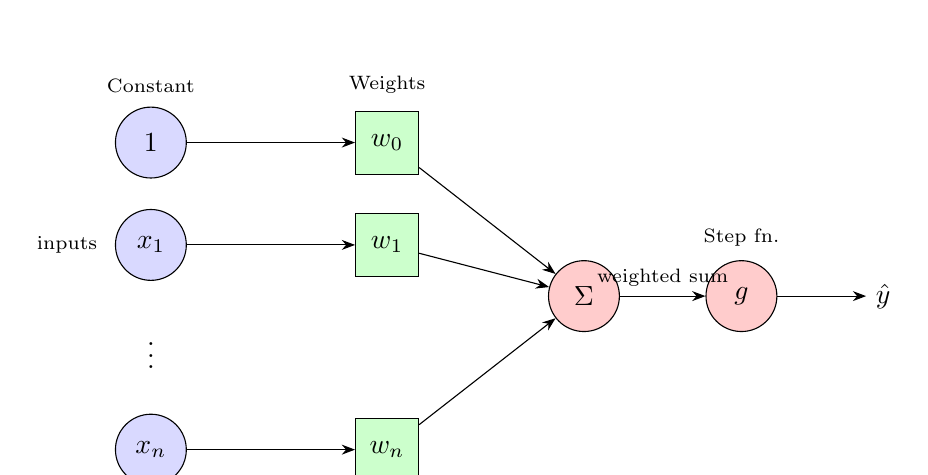
\begin{tikzpicture}[
        >=Stealth,
        neuron/.style={circle, draw, minimum size=0.9cm, fill=blue!15},
        weight/.style={rectangle, draw, minimum size=0.8cm, fill=green!20},
        op/.style={circle, draw, minimum size=0.9cm, fill=red!20}
    ]
        \node[neuron] (bias) at (0, 2.6)  {$1$};
        \node[neuron] (x1)   at (0, 1.3)  {$x_1$};
        \node          (dots) at (0, 0)    {$\vdots$};
        \node[neuron] (xn)   at (0, -1.3) {$x_n$};

        \node[weight] (w0) at (3.0, 2.6)  {$w_0$};
        \node[weight] (w1) at (3.0, 1.3)  {$w_1$};
        \node[weight] (wn) at (3.0, -1.3) {$w_n$};

        \node[op] (sum) at (5.5, 0.65) {$\Sigma$};
        \node[op] (act) at (7.5, 0.65) {$g$};
        \node     (out) at (9.3, 0.65) {$\hat{y}$};

        \draw[->] (bias) -- (w0);
        \draw[->] (x1)   -- (w1);
        \draw[->] (xn)   -- (wn);
        \draw[->] (w0)   -- (sum);
        \draw[->] (w1)   -- (sum);
        \draw[->] (wn)   -- (sum);
        \draw[->] (sum)  -- node[above, font=\scriptsize]{weighted sum} (act);
        \draw[->] (act)  -- (out);

        \node[above=0.05cm of bias, font=\scriptsize]{Constant};
        \node[left=0.1cm  of x1,   font=\scriptsize]{inputs};
        \node[above=0.1cm of w0,   font=\scriptsize]{Weights};
        \node[above=0.05cm of act, font=\scriptsize]{Step fn.};
    \end{tikzpicture}
    \caption{Perceptron: inputs are multiplied by learned weights, summed, and passed through an activation function.}\label{fig:perceptron}
\end{figure}


\section{Activation Functions}

Activation functions introduce \textbf{non-linearity} into the network. Without them, stacking linear layers collapses to a single linear transformation, making the model incapable of representing non-linear decision boundaries. They are a crucial element of every architecture.

\begin{itemize}
    \item \textbf{Sigmoid}: $\sigma(x) = \dfrac{1}{1+e^{-x}}$\\
        Output in $(0,1)$; historically widespread but suffers from vanishing gradients at saturation.

    \item \textbf{Tanh}: $\tanh(x)$\\
        Zero-centered; output in $(-1,1)$; generally preferred over sigmoid in hidden layers.

    \item \textbf{ReLU} (Rectified Linear Unit): $\max(0, x)$\\
        Sparse activations, computationally cheap; the default choice in modern architectures.

    \item \textbf{Leaky ReLU}: $\max(0.1x,\, x)$\\
        Mitigates the dying ReLU problem by allowing a small gradient for negative inputs.

    \item \textbf{ELU} (Exponential Linear Unit):
    \[
        \mathrm{ELU}(x) = \begin{cases} x & x \geq 0 \\ \alpha(e^x - 1) & x < 0 \end{cases}
    \]
    Smooth for negative inputs; can push mean activations toward zero.

    \item \textbf{Maxout}: $\max(w_1^T x + b_1,\; w_2^T x + b_2)$\\
        Generalizes ReLU and Leaky ReLU; learns the activation shape at the cost of doubling the parameter count.
\end{itemize}


\section{From Perceptron to Neural Networks}

\subsection{The Multi-Layer Idea}

The goal is to build a \textbf{larger, non-linear model}. The key idea: concatenate many perceptron systems and insert a \textbf{non-linear activation function} between computation layers. A two-layer network (one hidden layer) computes:
\[
    \mathbf{y}_1 = \mathbf{x} W_1 + \mathbf{b}_1, \qquad
    \mathbf{y}_2 = \phi(\mathbf{y}_1)\, W_2 + \mathbf{b}_2, \qquad
    \hat{\mathbf{y}} = s(\mathbf{y}_2)
\]
where $\phi$ is a non-linear activation (e.g., ReLU) and $s$ is the output activation (e.g., softmax for classification).

\subsection{Dimensions}

For a problem with $F$ input features, $H$ hidden neurons, and $C$ output classes:
\begin{itemize}
    \item $\mathbf{x} \in \R^{1 \times F}$, $W_1 \in \R^{F \times H}$, $\mathbf{b}_1 \in \R^{1 \times H}$, $\mathbf{y}_1 \in \R^{1 \times H}$
    \item $W_2 \in \R^{H \times C}$, $\mathbf{b}_2 \in \R^{1 \times C}$, $\mathbf{y}_2 \in \R^{1 \times C}$
\end{itemize}

\textit{Example}: a $28{\times}28$ grayscale image ($F=784$), $H=1024$ hidden neurons, $C=3$ classes:
\[
    \underbrace{\mathbf{x}}_{1 \times 784}
    \cdot\underbrace{W_1}_{784 \times 1024}
    + \underbrace{\mathbf{b}_1}_{1 \times 1024}
    = \underbrace{\mathbf{y}_1}_{1 \times 1024}
    \;\xrightarrow{\;\mathrm{ReLU}\;}\;
    \underbrace{W_2}_{1024 \times 3}
    + \underbrace{\mathbf{b}_2}_{1 \times 3}
    = \underbrace{\mathbf{y}_2}_{1 \times 3}
    \;\to\; s(\mathbf{y}_2)
\]

\subsection{Multilayer Perceptron (MLP)}

The \textbf{Multilayer Perceptron} (MLP) extends this to an arbitrary number of stacked hidden layers. For input $x = (\chi_1, \ldots, \chi_p)^T$:
\begin{enumerate}
    \item \textbf{Hidden layer} with weight matrix $W^h$ and activation $\sigma$:
    \[
        u_j = \sum_i W^h_{ji}\,\chi_i, \qquad h_j = \sigma(u_j)
    \]
    \item \textbf{Output layer} with weight matrix $W^y$:
    \[
        v_k = \sum_j W^y_{kj}\,h_j, \qquad y_k = \sigma(v_k)
    \]
\end{enumerate}

The network is \textbf{fully connected}: every neuron in layer $\ell$ connects to every neuron in layer $\ell+1$.

\begin{figure}[h]
    \centering
    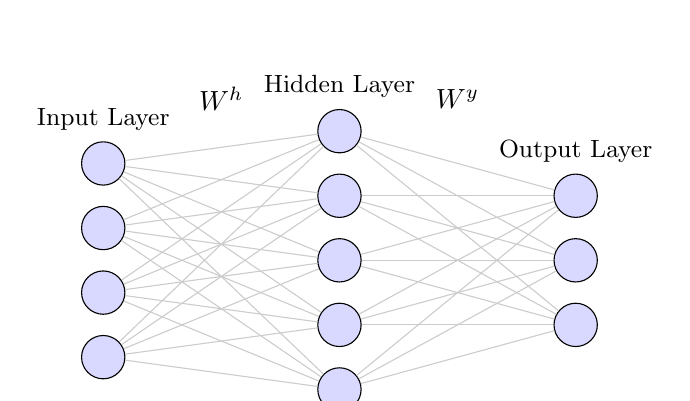
\begin{tikzpicture}[
        >=Stealth,
        neuron/.style={circle, draw, minimum size=0.55cm, fill=blue!15}
    ]
        \def\layersep{3.0cm}
        \def\nodesep{0.82cm}

        \foreach \i in {1,...,4}
            \node[neuron] (I\i) at (0, {(-\i+2.5)*\nodesep}) {};
        \foreach \i in {1,...,5}
            \node[neuron] (H\i) at (\layersep, {(-\i+3)*\nodesep}) {};
        \foreach \i in {1,...,3}
            \node[neuron] (O\i) at (2*\layersep, {(-\i+2)*\nodesep}) {};

        \foreach \i in {1,...,4}
            \foreach \j in {1,...,5}
                \draw[gray!40] (I\i) -- (H\j);
        \foreach \i in {1,...,5}
            \foreach \j in {1,...,3}
                \draw[gray!40] (H\i) -- (O\j);

        \node[above=0.3cm] at (0,           {1.5*\nodesep}) {\small Input Layer};
        \node[above=0.3cm] at (\layersep,   {2.0*\nodesep}) {\small Hidden Layer};
        \node[above=0.3cm] at (2*\layersep, {1.0*\nodesep}) {\small Output Layer};
        \node at (0.5*\layersep, {2.5*\nodesep}) {$W^h$};
        \node at (1.5*\layersep, {2.5*\nodesep}) {$W^y$};
    \end{tikzpicture}
    \caption{Multilayer Perceptron with one hidden layer.}\label{fig:mlp}
\end{figure}


\section{Training Neural Networks}

\subsection{Training and Testing Stages}

Neural network training proceeds in two distinct phases:
\begin{itemize}
    \item \textbf{Training stage}: input data is passed through the network and compared to the ground truth. The network parameters are adjusted to minimize the discrepancy.
    \item \textbf{Testing stage}: new, unseen input is passed through the \textit{trained} (frozen) network to produce a prediction (best guess).
\end{itemize}

\subsection{Forward and Backward Pass}

Each training step consists of two passes:
\begin{enumerate}
    \item \textbf{Forward pass}: propagate the input through the network to compute a prediction.
    \item \textbf{Backward pass (backpropagation)}: compute the loss between prediction and ground truth; propagate the error signal backward through the network via the chain rule; update weights to reduce the error.
\end{enumerate}


\section{Loss Functions}

A loss function quantifies the discrepancy between the network's prediction $p$ and the ground truth $t$. The choice is \textbf{task-dependent}.

\subsection{Standard Loss Functions}

\begin{enumerate}
    \item \textbf{Regression} --- Mean Squared Error (MSE):
    \[
        \mathrm{MSE} = \frac{1}{n}\sum \bigl(y - \hat{y}\bigr)^2
    \]

    \item \textbf{Binary classification} --- Binary Cross-Entropy (BCE):
    \[
        \mathrm{BCE}(t, p) = -\bigl(t \cdot \log(p) + (1-t) \cdot \log(1-p)\bigr)
    \]

    \item \textbf{Multiclass classification} --- Categorical Cross-Entropy (CCE):
    \[
        \mathrm{CCE}(p, t) = -\sum_{c=1}^{C} t_{o,c}\,\log(p_{o,c})
    \]
\end{enumerate}

\subsection{Cross-Entropy and Information Theory}

Cross-entropy loss derives from the notion of \textbf{entropy} $H(X)$, which measures the uncertainty of a probability distribution:
\[
    H(X) = \begin{cases}
        -\displaystyle\int_x p(x)\log p(x)\,dx & \text{if } X \text{ is continuous} \\[8pt]
        -\displaystyle\sum_x p(x)\log p(x)     & \text{if } X \text{ is discrete}
    \end{cases}
\]
(Logarithm in base 2.)

\begin{itemize}
    \item Higher $H(X)$ $\Rightarrow$ greater uncertainty in the distribution.
    \item A \textbf{uniform} $p(x)$ $\Rightarrow$ maximum entropy (maximum uncertainty).
    \item A \textbf{Dirac delta} $p(x)$ $\Rightarrow$ minimum entropy (zero uncertainty).
\end{itemize}

Minimizing cross-entropy is equivalent to concentrating the predicted distribution on the correct class. Hence: \textbf{the lower the loss, the better the model}.

\subsection{Loss as an Optimization Objective}

Because loss functions are \textbf{differentiable}, the learning problem can be cast as an \textbf{optimization problem}.

\begin{tcolorbox}[colback=blue!5!white,colframe=blue!75!black,title=\textbf{Key Insight}]
By training the network, we want to find the weights that achieve \textbf{minimal loss}. The weight update algorithm is called \textbf{Gradient Descent}, implemented in practice via the \textbf{backpropagation procedure}.
\end{tcolorbox}


\section{Backpropagation and Gradient Descent}

\subsection{General Idea}

Backpropagation iteratively updates \textbf{weights} $w$ and \textbf{biases} $b$ to decrease the loss $J(w)$. The procedure decomposes into three sub-tasks:
\begin{enumerate}
    \item \textbf{Forward pass}: compute the network output and evaluate the loss.
    \item \textbf{Backward pass}: compute gradients $\partial J/\partial w$ by applying the chain rule layer by layer (from output to input).
    \item \textbf{Weight update}: subtract a fraction of the gradient from each weight. The fraction is controlled by the \textbf{learning rate} $\eta$ --- a critical hyperparameter.
\end{enumerate}

The update corresponds geometrically to moving in the direction of \textbf{steepest descent} on the loss surface.

\begin{figure}[h]
    \centering
    \begin{tikzpicture}
        \begin{axis}[
            width=7cm, height=5cm,
            xlabel={$w$}, ylabel={$J(w)$},
            axis lines=left,
            xmin=-0.5, xmax=4.5,
            ymin=-0.2, ymax=5.5,
            xtick=\empty, ytick=\empty,
            clip=false
        ]
            \addplot[blue!60!black, thick, domain=0:4.2, samples=100] {(x-1)^2 + 0.2};
            \addplot[mark=*, mark size=3pt, black] coordinates {(3.6, 6.76)};
            \node[right, font=\small] at (axis cs:3.6, 5.2) {Initial weight};
            \node[below, font=\small] at (axis cs:1.0, 0.2) {$J_{\min}(w)$};
            \draw[->, thick, dashed, black!70] (axis cs:3.5, 5.05) -- (axis cs:2.7, 2.89);
            \draw[->, thick, dashed, black!70] (axis cs:2.7, 2.89) -- (axis cs:1.9, 0.92);
            \draw[->, thick, dashed, black!70] (axis cs:1.9, 0.92) -- (axis cs:1.2, 0.24);
            \node[right, font=\scriptsize, black!60] at (axis cs:3.2, 4.0) {Gradient};
        \end{axis}
    \end{tikzpicture}
    \caption{Gradient descent on a 1D loss surface. Each step moves in the direction of the negative gradient toward the global minimum.}\label{fig:gd}
\end{figure}

\subsection{Batch Gradient Descent}

\begin{enumerate}
    \item Initialize weights randomly: $w \sim \mathcal{N}(0, \sigma^2)$.
    \item Repeat until convergence:
    \begin{enumerate}
        \item Compute the gradient $\dfrac{\partial J(w)}{\partial w}$ over the \emph{entire} training set.
        \item Update: $w \leftarrow w - \eta\,\dfrac{\partial J(w)}{\partial w}$.
    \end{enumerate}
    \item Return $w$.
\end{enumerate}

\textbf{Drawback}: computing the gradient over all training samples is very expensive when the dataset contains millions of examples.

\subsection{Stochastic Gradient Descent (SGD)}

SGD reduces the cost by estimating the gradient from a \textit{single} training sample $i$ at each step:
\begin{enumerate}
    \item Initialize weights randomly: $w \sim \mathcal{N}(0, \sigma^2)$.
    \item Repeat until convergence:
    \begin{enumerate}
        \item Pick a single data point $i$.
        \item Compute the gradient $\dfrac{\partial J_i(w)}{\partial w}$.
        \item Update: $w \leftarrow w - \eta\,\dfrac{\partial J(w)}{\partial w}$.
    \end{enumerate}
    \item Return $w$.
\end{enumerate}

\textbf{Drawback}: the gradient estimate is very noisy since it relies on a single instance.

\subsection{Mini-Batch Gradient Descent}

Mini-batch gradient descent is the standard approach in practice --- the middle ground between batch GD and SGD:
\begin{enumerate}
    \item Initialize weights randomly: $w \sim \mathcal{N}(0, \sigma^2)$.
    \item Repeat until convergence:
    \begin{enumerate}
        \item Pick a batch $B$ of data points.
        \item Compute the averaged gradient:
        \[
            \frac{\partial J_B(w)}{\partial w} = \frac{1}{B}\sum_{k=1}^{B} \frac{\partial J_k(w)}{\partial w}
        \]
        \item Update: $w \leftarrow w - \eta\,\dfrac{\partial J(w)}{\partial w}$.
    \end{enumerate}
    \item Return $w$.
\end{enumerate}

\begin{tcolorbox}[colback=green!5!white,colframe=green!75!black]
    Mini-batch gradient descent yields \textbf{smoother convergence}, \textbf{more stable gradients}, and allows for \textbf{larger learning rates} compared to pure SGD --- making it the default optimization strategy in deep learning.
\end{tcolorbox}











% ========================================
\part{Backpropagation: Derivation and Training Dynamics}
% ========================================

\section{Expressive Capacity of Multilayer Networks}

\subsection{What a Single Perceptron Can Represent}

A perceptron with $n$ inputs defines a hyperplane of dimension $n-1$ that partitions the input space into two half-spaces:
\[
    \sum_{i=1}^n w_i x_i - t = 0
\]
This limits its classification ability to \textbf{linearly separable} problems. The canonical failure case is XOR --- no values $w_0, w_1, w_2$ can satisfy the four constraints simultaneously.

\subsection{Capacity with Hidden Layers}

Adding hidden layers dramatically increases expressive power. In the two-dimensional case:

\begin{itemize}
    \item Each hidden neuron defines a boundary line (half-plane).
    \item With $h$ hidden neurons, the output neuron takes their conjunction: three neurons yield a triangle, four a quadrilateral, and so on.
\end{itemize}

The following theorems quantify this:

\begin{theorem}[Huang \& Lipmann, 1988]
A feed-forward network with a single hidden layer can approximate \textit{almost all} separation surfaces between two classes. The qualifier ``almost all'' means that by adding a second output neuron, non-convex and disconnected regions become representable too.
\end{theorem}

\begin{theorem}[Gibson \& Lowan, 1990]
There exist regions that a single-hidden-layer network cannot approximate --- for example, two triangular regions that touch at exactly one point.
\end{theorem}

\begin{theorem}[Lipmann, 1987]
A feed-forward network with \textbf{two} hidden layers can approximate any region in input space. Approximation accuracy is controlled by the number of neurons in the intermediate layers.
\end{theorem}

\begin{remark}
These results are existence theorems, not constructive recipes. In practice, there are no fixed rules for choosing architecture; empirical heuristics and cross-validation guide the design.
\end{remark}


\section{Formal Derivation of Backpropagation}

\subsection{Setup and Notation}

Consider a two-layer feed-forward network with $n$ inputs, $h$ hidden neurons, and $q$ output neurons. Let $g$ be a differentiable activation function (e.g.\ the logistic). Define:

\begin{center}
\renewcommand{\arraystretch}{1.4}
\begin{tabular}{ll}
    $I_i$      & $i$-th input \\
    $w_{ji}$   & weight from input $i$ to hidden neuron $j$ \\
    $a_j = \displaystyle\sum_{i=1}^n w_{ji}\,I_i$     & pre-activation of hidden neuron $j$ \\
    $Z_j = g(a_j)$                                     & output of hidden neuron $j$ \\
    $W_{kj}$   & weight from hidden neuron $j$ to output neuron $k$ \\
    $a_k = \displaystyle\sum_{j=1}^h W_{kj}\,Z_j$     & pre-activation of output neuron $k$ \\
    $O_k = g(a_k)$                                     & output of network for class $k$
\end{tabular}
\end{center}

The squared error for a single training example with target $y_k$:
\[
    E(W) = \frac{1}{2}\sum_{k=1}^{q} {\bigl(y_k - O_k\bigr)}^{2}
\]

\subsection{Derivatives for the Output Layer}

We want $\partial E / \partial W_{kj}$. By the chain rule:
\[
    \frac{\partial E}{\partial W_{kj}} = \frac{\partial E}{\partial O_k}\cdot\frac{\partial O_k}{\partial a_k}\cdot\frac{\partial a_k}{\partial W_{kj}}
\]

Computing each factor:
\[
    \frac{\partial E}{\partial O_k} = -(y_k - O_k), \qquad
    \frac{\partial O_k}{\partial a_k} = g'(a_k), \qquad
    \frac{\partial a_k}{\partial W_{kj}} = Z_j
\]

Define the \textbf{output delta}:
\[
    \delta_k \coloneqq (O_k - y_k)\,g'(a_k)
\]

Then:
\[
    \boxed{\frac{\partial E}{\partial W_{kj}} = \delta_k\,Z_j}
\]

The weight update (gradient descent) for the output layer is:
\[
    \Delta W_{kj} = -\eta\,\delta_k\,Z_j
\]

\subsection{Derivatives for the Hidden Layer}

We want $\partial E / \partial w_{ji}$. By the chain rule:
\[
    \frac{\partial E}{\partial w_{ji}} = \frac{\partial E}{\partial a_j}\cdot\frac{\partial a_j}{\partial w_{ji}}
\]

The second factor is simply $\partial a_j / \partial w_{ji} = I_i$. For the first factor we must account for the fact that $a_j$ feeds all $q$ output neurons through $Z_j$:
\[
    \frac{\partial E}{\partial a_j} = \sum_{k=1}^{q} \frac{\partial E}{\partial a_k}\cdot\frac{\partial a_k}{\partial Z_j}\cdot\frac{\partial Z_j}{\partial a_j}
    = \sum_{k=1}^{q} \delta_k\,W_{kj}\cdot g'(a_j)
    = g'(a_j)\sum_{k=1}^{q} \delta_k\,W_{kj}
\]

Define the \textbf{hidden delta}:
\[
    \delta_j \coloneqq g'(a_j)\sum_{k=1}^{q} \delta_k\,W_{kj}
\]

Then:
\[
    \boxed{\frac{\partial E}{\partial w_{ji}} = \delta_j\,I_i}
\]

The weight update for the hidden layer is:
\[
    \Delta w_{ji} = -\eta\,\delta_j\,I_i
\]

\subsection{General Weight Update Rule}

Both updates share the same structure. For any weight connecting neuron $q$ (input side) to neuron $p$ (output side):
\[
    \Delta W_{pq} = -\eta\,\delta_p \cdot V_q
\]
where $V_q$ is the activation value at the input neuron and $\delta_p$ is the error signal at the output neuron, computed by:

\begin{itemize}
    \item \textbf{Output layer}: $\delta_k = (O_k - y_k)\,g'(a_k)$
    \item \textbf{Hidden layer}: $\delta_j = g'(a_j)\displaystyle\sum_k \delta_k\,W_{kj}$ \quad (weighted sum of upstream deltas)
\end{itemize}

This recursive structure is what gives the algorithm its name: error signals $\delta$ are \emph{propagated backward}, from output to input, layer by layer.

\subsection{Algorithm}

\begin{algorithm}
\caption{Backpropagation (online, one training example per step)}
\begin{algorithmic}[1]
\STATE Initialize all weights randomly (small values).
\REPEAT
    \STATE \textbf{Forward pass}: present input $\mathbf{x}$; compute $a_j, Z_j, a_k, O_k$ for all hidden and output neurons; store activations.
    \STATE \textbf{Compute output deltas}: $\delta_k \leftarrow (O_k - y_k)\,g'(a_k)$ for all $k$.
    \STATE \textbf{Backpropagate}: $\delta_j \leftarrow g'(a_j)\sum_k \delta_k\,W_{kj}$ for all hidden neurons $j$.
    \STATE \textbf{Update output weights}: $W_{kj} \leftarrow W_{kj} - \eta\,\delta_k\,Z_j$.
    \STATE \textbf{Update hidden weights}: $w_{ji} \leftarrow w_{ji} - \eta\,\delta_j\,I_i$.
\UNTIL{convergence}
\end{algorithmic}
\end{algorithm}

\subsection{Complexity}

Computing the gradient via finite differences (difference quotient) costs $\mathcal{O}(W^2)$: for each of the $W$ weights, the network must be evaluated anew. Backpropagation reduces this to $\mathcal{O}(W)$ by reusing intermediate activations and computing all partial derivatives in a single backward sweep. This is the key efficiency gain that makes training large networks tractable.

An additional structural benefit is \textbf{locality}: the update $\Delta W_{pq}$ depends only on the activation at neuron $q$ and the delta at neuron $p$ --- exactly the two endpoints of the connection. This locality makes the algorithm trivially parallelizable.


\section{Optimization Challenges}

\subsection{Learning Rate Sensitivity}

The learning rate $\eta$ is a critical hyperparameter. Its effect is qualitatively different in two failure regimes:

\begin{itemize}
    \item $\eta$ \textbf{too small}: convergence is slow; training may require an impractical number of epochs.
    \item $\eta$ \textbf{too large}: the update overshoots the minimum, causing the weights to oscillate between two configurations without converging.
\end{itemize}

\subsection{Local Minima}

The loss surface of a deep network is non-convex, with many local minima. Gradient descent is only guaranteed to converge to a \emph{local} minimum; the outcome depends on the initialization. If the starting configuration $W^{(0)}$ is far from the global minimum, the algorithm may settle at a suboptimal solution.

\paragraph{Momentum.} A practical remedy is to add a \textbf{momentum term} that incorporates inertia from the previous step:
\[
    \Delta W^{(k)} = -\eta\,\frac{\partial E}{\partial W}\bigg|_{W^{(k)}} + \alpha\bigl(W^{(k)} - W^{(k-1)}\bigr)
\]
where $\alpha \in (0,1)$ is the momentum parameter (commonly $\alpha = 0.9$). The effect is to dampen oscillations in directions of high curvature and accelerate movement along low-curvature directions. Other global optimization strategies (simulated annealing, genetic algorithms, reactive Tabu search) can also be applied.

\subsection{Saturation}

When an activation function is in its saturated regime --- inputs far from zero for sigmoid or tanh --- its derivative $g'$ is nearly zero. Consequently, $\delta \propto g'$ is nearly zero as well, and weight updates become negligibly small. Training effectively stalls.

\textbf{Mitigation}: initialize weights to small random values. Near zero, the activation functions are approximately linear and their derivatives are large, so gradients are well-conditioned at the start of training. As learning proceeds, weights grow only as needed.


\section{Generalization}

\subsection{Definition}

A network's \textbf{generalization capacity} is its ability to correctly classify inputs \emph{not} seen during training. Minimizing training loss is a means to an end, not the end itself. A model that perfectly memorizes training examples but fails on new ones has not learned anything useful.

\subsection{Overfitting}

\textbf{Overfitting} (also called overtraining) occurs when the network has been trained for too many epochs: it has memorized the training patterns, including their noise, at the expense of flexibility on unseen inputs. The telltale sign is a divergence between training and test error:

\begin{itemize}
    \item \textbf{Training error}: monotonically decreasing.
    \item \textbf{Test error}: initially decreasing, then increasing after some epoch $e_0$.
\end{itemize}

The optimal stopping point is $e_0$, before the test error begins to rise. This technique is known as \textbf{early stopping}.

\begin{tcolorbox}[colback=orange!5!white,colframe=orange!75!black,title=\textbf{Key Principle}]
Minimizing training error is \textbf{not} equivalent to training a good neural network. The minimum training error does not correspond to the best generalization. Overfitting must always be monitored.
\end{tcolorbox}


\section{Cross-Validation Strategies}

In practice, labeled data is limited. The following strategies manage the training-evaluation tradeoff under this constraint.

\subsection{Resubstitution}

Train and evaluate on the \emph{same} set (all available data). This produces an \textbf{optimistic} (lower-bound) error estimate: the model has already seen every example during training, so measured error is artificially low.

\subsection{Holdout}

Randomly partition the dataset into two disjoint halves: one for training, one for testing. This provides an \textbf{upper-bound} error estimate, since the model sees only half the data during training. The result is sensitive to the particular partition chosen.

\subsection{Averaged Holdout}

Repeat the holdout procedure multiple times with different random partitions and average the resulting errors. This reduces the variance introduced by a single arbitrary split. Partitions can be sampled randomly or enumerated exhaustively.

\subsection{Leave-One-Out (LOO)}

Given $N$ examples, train on $N-1$ and test on the single excluded example; repeat for every example and average. This maximally utilizes the available data and provides a near-unbiased error estimate. The computational cost is $N$ training runs, which can be prohibitive for large datasets or slow-converging models.

\subsection{$k$-Fold Cross-Validation}

A practical compromise between holdout and LOO. Partition the data into $k$ disjoint segments (folds) of equal size. For each fold:
\begin{enumerate}
    \item Train on the remaining $k-1$ folds.
    \item Evaluate on the held-out fold.
\end{enumerate}
Average the $k$ test errors. Leave-one-out corresponds to $k = N$. A common choice in practice is $k = 5$ or $k = 10$, balancing computational cost against variance.

\begin{center}
\renewcommand{\arraystretch}{1.3}
\begin{tabular}{lccc}
    \hline
    \textbf{Method} & \textbf{Training size} & \textbf{Bias} & \textbf{Variance} \\
    \hline
    Resubstitution  & $N$       & High (optimistic) & Low \\
    Holdout         & $N/2$     & Moderate          & High \\
    Averaged Holdout & $N/2$   & Moderate          & Lower \\
    Leave-One-Out   & $N-1$     & Low               & High \\
    $k$-Fold        & $(k-1)N/k$ & Low--moderate    & Moderate \\
    \hline
\end{tabular}
\end{center}


\section{When to Use Neural Networks}

Neural networks are an appropriate choice when:

\begin{enumerate}
    \item \textbf{The problem is instance-based}: examples are given as (attributes, class) pairs. Raw inputs should be preprocessed --- real-valued features scaled to $[0,1]$, discrete features one-hot encoded.
    \item \textbf{The training set is large}: generalization improves monotonically with data; small datasets favor simpler, more data-efficient models.
    \item \textbf{Long training times are acceptable}: iterative optimization over large parameter spaces is inherently expensive.
    \item \textbf{Interpretability is not required}: the learned weight matrices are opaque; if human-readable discriminant functions are needed, decision trees or linear models are preferable.
\end{enumerate}



% ========================================
\part{Convolutional Neural Networks}
% ========================================

\section{Regularization}

Deep networks have high expressive power and will readily memorize training data. \textbf{Regularization} constrains the optimization problem to encourage generalization on unseen inputs, rather than overfitting to training noise.

\subsection{The Bias-Variance Trade-off}

Model quality is governed by two competing sources of error:

\begin{itemize}
    \item \textbf{Bias}: error from overly simplistic assumptions; the model underfits the data.
    \item \textbf{Variance}: error from excessive sensitivity to training data; the model overfits.
\end{itemize}

As model complexity increases, bias decreases but variance grows. The optimal model lives at the minimum of their sum. Deep networks are high-variance models by default --- regularization is what keeps them on the right side of this trade-off.

\subsection{Early Stopping}

Stop training as soon as the validation loss stops improving. In practice:
\begin{itemize}
    \item \textbf{Training loss}: monotonically decreasing.
    \item \textbf{Validation loss}: decreases early, then rises as overfitting begins.
\end{itemize}
The checkpoint at the minimum validation loss is retained as the final model. This is the simplest and most widely used regularizer.

\subsection{L2 Regularization (Ridge / Weight Decay)}

Add an L2 penalty on all weights to the loss:
\[
    \mathcal{L}' = \mathcal{L} + \frac{\beta}{2}\|W\|_2^2 = \mathcal{L} + \frac{\beta}{2}\sum_i w_i^2
\]
where $\beta > 0$ is the penalty factor. The added term penalizes large weights, forcing the network to distribute the learned signal evenly and discouraging any single connection from dominating. In the gradient update this appears as a constant multiplicative decay on weights at each step, hence the name \emph{weight decay}.

\subsection{Dropout}

\textbf{Dropout} prevents neurons from \emph{co-adapting} --- relying on the presence of specific other neurons and thus becoming brittle. During each training step, each neuron is independently retained with probability $p$ (typically $p \geq 0.5$ for later layers; higher for early layers and input) and dropped (set to zero) with probability $1-p$.

The effect: each training step is equivalent to training a different sub-network. At test time all neurons are active but their outputs are scaled by $p$ to match the expected activation. This ensemble-like behaviour provides strong regularization at negligible cost.

\subsection{Batch Normalization}

As training progresses, the distribution of inputs to each hidden layer shifts as the parameters of preceding layers change --- a phenomenon called \textbf{internal covariate shift}. Batch normalization (Ioffe \& Szegedy, ICML 2015) mitigates this by normalizing each feature dimension across the current mini-batch:
\[
    \hat{x}^{(k)} = \frac{x^{(k)} - \mathbb{E}[x^{(k)}]}{\sqrt{\mathrm{Var}[x^{(k)}]}}
\]
To preserve representational power, two learnable parameters $\gamma^{(k)}$ and $\beta^{(k)}$ are introduced per feature:
\[
    y^{(k)} = \gamma^{(k)}\hat{x}^{(k)} + \beta^{(k)}
\]
Batch normalization is inserted between the linear transformation and the activation function. It accelerates training, acts as a mild regularizer, and is practically indispensable in very deep architectures.


\section{Convolutional Neural Networks}

\subsection{Motivation: Receptive Fields and Weight Sharing}

The mammalian visual cortex is organized so that individual neurons respond only to stimuli within a restricted region of the visual field --- their \textbf{receptive field}. Nearby neurons have overlapping receptive fields that tile the entire visual scene. \textbf{Convolutional Neural Networks} (CNNs) are loosely inspired by this architecture.

The fundamental observation is that the same local pattern detector (e.g., an edge detector) is useful everywhere in an image --- there is no reason to learn a separate detector for each spatial location. CNNs exploit this by \textbf{sharing weights} across space: a single filter is convolved with the entire input, producing a \textbf{feature map} that encodes where the detected pattern appears.

\subsection{The Convolution Operation}

A filter (kernel) $K$ of size $k \times k$ is slid over the input with a chosen \textbf{stride} $s$. At each position, the element-wise product of the filter and the corresponding input patch is summed to produce a single output value. For a 2D input $X$ and filter $K$:
\[
    (X * K)[i,j] = \sum_{m=0}^{k-1}\sum_{n=0}^{k-1} X[i \cdot s + m,\; j \cdot s + n] \cdot K[m,n]
\]

\begin{example}
A $5 \times 5$ input convolved with a $3 \times 3$ filter at stride 1 produces a $3 \times 3$ feature map. The filter is positioned at each valid location, element-wise multiplied with the input patch, and summed:
\[
\begin{pmatrix}1&1&1&0&0\\0&1&1&1&0\\0&0&1&1&1\\0&0&1&1&0\\0&1&1&0&0\end{pmatrix}
*
\begin{pmatrix}1&0&1\\0&1&0\\1&0&1\end{pmatrix}
=
\begin{pmatrix}4&3&4\\2&4&3\\2&3&4\end{pmatrix}
\]
\end{example}

\paragraph{Output spatial size.} For an input of height/width $H$, filter size $k$, stride $s$, and zero-padding $p$:
\[
    H_{\text{out}} = \left\lfloor \frac{H + 2p - k}{s} \right\rfloor + 1
\]

\subsection{Feature Maps and Filters}

A convolutional layer applies $d$ different filters to the same input, producing $d$ feature maps stacked along the \textbf{depth} dimension (not to be confused with the depth of the network). Each filter learns to detect a distinct local pattern.

\begin{itemize}
    \item \textbf{Shallow filters} (early layers): detect simple patterns such as oriented edges and color gradients.
    \item \textbf{Deeper filters}: combine the activations of previous layers to detect increasingly abstract patterns --- textures, object parts, complete objects.
\end{itemize}

A layer therefore maps an input volume of shape $H \times W \times d_{\text{in}}$ to an output volume of shape $H' \times W' \times d_{\text{out}}$, where $d_{\text{out}}$ equals the number of filters.

\subsection{Non-linearity}

After each convolution, a non-linear activation is applied element-wise. In modern CNNs this is almost universally \textbf{ReLU}:
\[
    g(z) = \max(0, z)
\]
ReLU is applied independently to each element of the feature map, setting all negative values to zero. Without non-linearity, stacked convolutions would collapse to a single linear filter.

\subsection{Pooling}

Pooling layers reduce spatial dimensions, thereby:
\begin{itemize}
    \item decreasing the number of parameters and computation,
    \item introducing limited spatial invariance (small translations of the input produce the same output),
    \item controlling overfitting.
\end{itemize}

The most common variant is \textbf{max pooling}: a $k \times k$ window slides over the feature map with stride $s$ and outputs the maximum value in each window. A $2 \times 2$ max pool with stride 2 is the standard, halving both spatial dimensions.

\subsection{Fully Connected Layer and Softmax}

After a sequence of convolution and pooling operations, the spatial dimensions are small enough that the feature map is \textbf{flattened} into a vector and passed through one or more fully connected layers. The final FC layer has as many neurons as there are classes.

For multiclass classification, the output is passed through \textbf{softmax}:
\[
    P(y = j \mid \mathbf{x}) = \frac{e^{z_j}}{\displaystyle\sum_{k=1}^{C} e^{z_k}}
\]
which converts raw scores $\mathbf{z}$ into a proper probability distribution over $C$ classes. Combined with categorical cross-entropy loss, softmax is the standard output for classification CNNs.

\subsection{Standard Architecture Pattern}

The canonical CNN architecture stacks convolutional blocks followed by fully connected layers:
\[
    \text{INPUT} \to {\bigl[{[\text{CONV} \to \text{ReLU}]}^{N} \to \text{POOL}\bigr]}^{M} \to {[\text{FC} \to \text{ReLU}]}^{K} \to \text{FC (softmax)}
\]
Typical choices: $N \leq 3$, $M \geq 1$, $K \leq 2$. The convolutional blocks learn spatial features; the FC layers perform classification.

\begin{tcolorbox}[colback=blue!5!white,colframe=blue!75!black,title=\textbf{Summary: CNN Layers}]
\begin{tabular}{lll}
    \textbf{Layer} & \textbf{Operation} & \textbf{Purpose} \\
    \hline
    CONV   & Sliding dot product with shared filters & Local feature extraction \\
    ReLU   & $\max(0, x)$ elementwise & Non-linearity \\
    POOL   & Max/avg over spatial window & Downsampling, invariance \\
    BN     & Normalize by batch statistics & Training stability \\
    FC     & Matrix multiply + bias & Classification / regression \\
    Softmax & Normalized exponential & Probability over classes \\
\end{tabular}
\end{tcolorbox}


\section{Landmark Architectures}

The ImageNet Large Scale Visual Recognition Challenge (ILSVRC) catalyzed a decade of architectural innovation. The following architectures represent the major milestones, each introducing a design principle that influenced the field.

\subsection{LeNet (1998)}

Developed by LeCun et al.\ for handwritten digit recognition on MNIST ($28 \times 28$ grayscale, 10 classes, 60k training examples). LeNet established the canonical pattern of interleaved convolution and subsampling:

\begin{align*}
    &\text{INPUT } (32\times32) \;\to\; C_1\;(6 @ 28\times28) \;\to\; S_2\;(6 @ 14\times14) \;\to\; C_3\;(16 @ 10\times10) \\
    &\to\; S_4\;(16 @ 5\times5) \;\to\; F_5\;(120) \;\to\; F_6\;(84) \;\to\; \text{OUTPUT }(10)
\end{align*}

Filters were $5 \times 5$ at stride 1; subsampling was average pooling $2 \times 2$ at stride 2; activation functions were sigmoid/tanh.

\subsection{AlexNet (2012)}

AlexNet (Krizhevsky et al.) won ILSVRC 2012 with a top-5 error of 15.3\%, compared to 26\% for the runner-up. It was the first deep CNN applied at scale to ImageNet:

\begin{itemize}
    \item 5 convolutional layers + 3 fully connected layers; 60 million parameters.
    \item \textbf{First use of ReLU} in a competitive CNN --- replacing sigmoid/tanh and substantially accelerating training.
    \item \textbf{Dropout} (rate 0.5) on FC layers to control overfitting.
    \item Data augmentation (random crops, horizontal flips, color jitter).
    \item Trained on two GTX 580 GPUs for one week.
    \item Hyperparameters: SGD with momentum 0.9, learning rate $10^{-2}$ (manually decayed), L2 weight decay $5 \times 10^{-4}$, mini-batch 128.
\end{itemize}

\textbf{Architecture} (for input $227 \times 227 \times 3$):
\begin{enumerate}
    \item $\text{CONV}_1$: 96 filters, $11\times11$, stride 4 $\to$ $55\times55\times96$; MAX POOL $3\times3$ s2 $\to$ $27\times27\times96$
    \item $\text{CONV}_2$: 256 filters, $5\times5$, pad 2 $\to$ $27\times27\times256$; MAX POOL $\to$ $13\times13\times256$
    \item $\text{CONV}_3$: 384 filters, $3\times3$, pad 1 $\to$ $13\times13\times384$
    \item $\text{CONV}_4$: 384 filters, $3\times3$, pad 1 $\to$ $13\times13\times384$
    \item $\text{CONV}_5$: 256 filters, $3\times3$, pad 1 $\to$ $13\times13\times256$; MAX POOL $\to$ $6\times6\times256$
    \item FC6: 4096 neurons; FC7: 4096 neurons; FC8: 1000 neurons (class scores)
\end{enumerate}

\subsection{ZFNet (2013)}

Won ILSVRC 2013. Zeiler \& Fergus improved AlexNet by:
\begin{itemize}
    \item reducing the first convolution from $11\times11$ stride 4 to $7\times7$ stride 2 (finer spatial resolution early on),
    \item expanding the number of feature maps in the middle convolutional layers.
\end{itemize}
ZFNet also introduced \textbf{deconvolution-based visualization} to understand which input patterns activate each filter, providing the first systematic tool for inspecting what CNNs learn.

\subsection{VGGNet (2014)}

Runner-up at ILSVRC 2014 (Simonyan \& Zisserman). VGGNet's central thesis: \textbf{depth alone, with small filters, drives performance}. Design rules:
\begin{itemize}
    \item All convolutions are $3 \times 3$ at stride 1, padding 1.
    \item All pooling is $2 \times 2$ max pooling at stride 2.
    \item 16 weight layers (VGG-16) or 19 (VGG-19); 138 million parameters.
\end{itemize}

Two stacked $3 \times 3$ convolutions have the same receptive field as one $5 \times 5$, but fewer parameters and an extra non-linearity. Three $3 \times 3$ convolutions match a $7 \times 7$ receptive field with a further reduction in parameters. This insight --- \emph{replace large filters with stacks of small ones} --- became a standard architectural principle.

\textbf{Limitation}: most memory is consumed by early convolutional layers; most parameters reside in the late FC layers (two FC layers of 4096 units each account for the majority of the 138M parameters).

\subsection{GoogLeNet / Inception (2014)}

Won ILSVRC 2014 (Szegedy et al., Google). The central innovation is the \textbf{Inception module}: rather than choosing a single filter size, apply $1\times1$, $3\times3$, and $5\times5$ convolutions and $3\times3$ max pooling \emph{in parallel} on the same input, then concatenate their outputs along the depth dimension.

\begin{itemize}
    \item \textbf{$1 \times 1$ convolutions} (bottleneck projections) reduce channel depth before the expensive $3\times3$ and $5\times5$ convolutions, dramatically cutting computation.
    \item 22 layers total; only 5 million parameters (vs.\ AlexNet's 60M) --- \textbf{12$\times$ fewer}.
    \item No large FC layers; replaced by \textbf{global average pooling}, eliminating the parameter bottleneck.
    \item Two \textbf{auxiliary classifiers} attached at intermediate layers combat vanishing gradients during training and provide additional regularization.
\end{itemize}

Later versions (v2, v3, v4) refined the inception blocks with further factorization (e.g., replacing $5\times5$ with two $3\times3$, or $n\times1$ followed by $1\times n$) and incorporated batch normalization.

\subsection{ResNet (2015)}

Won ILSVRC 2015 with 3.57\% top-5 error --- surpassing human-level performance (5.1\%). Developed by He et al.\ (Microsoft Research). ResNet's contribution: \textbf{residual (skip) connections} that make very deep networks trainable.

\paragraph{The residual block.} Instead of learning the mapping $H(\mathbf{x})$ directly, the block learns the \textbf{residual} $F(\mathbf{x}) = H(\mathbf{x}) - \mathbf{x}$, and the skip connection adds the input back:
\[
    H(\mathbf{x}) = F(\mathbf{x}) + \mathbf{x}
\]

\begin{figure}[h]
    \centering
    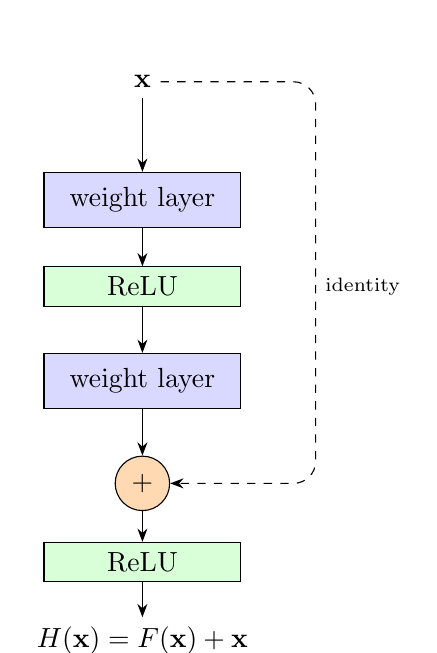
\begin{tikzpicture}[>=Stealth, node distance=1cm]
        \node (x)    at (0, 0)   {$\mathbf{x}$};
        \node[draw, rectangle, fill=blue!15, minimum width=2.5cm, minimum height=0.7cm]
              (w1)   at (0, -1.5) {weight layer};
        \node[draw, rectangle, fill=green!15, minimum width=2.5cm, minimum height=0.5cm]
              (r1)   at (0, -2.6) {ReLU};
        \node[draw, rectangle, fill=blue!15, minimum width=2.5cm, minimum height=0.7cm]
              (w2)   at (0, -3.8) {weight layer};
        \node[draw, circle, fill=orange!30, minimum size=0.6cm]
              (add)  at (0, -5.1) {$+$};
        \node[draw, rectangle, fill=green!15, minimum width=2.5cm, minimum height=0.5cm]
              (r2)   at (0, -6.1) {ReLU};
        \node (out)  at (0, -7.1) {$H(\mathbf{x}) = F(\mathbf{x}) + \mathbf{x}$};

        \draw[->] (x)   -- (w1);
        \draw[->] (w1)  -- (r1);
        \draw[->] (r1)  -- (w2);
        \draw[->] (w2)  -- (add);
        \draw[->] (add) -- (r2);
        \draw[->] (r2)  -- (out);

        % Skip connection
        \draw[->, rounded corners=8pt, dashed]
            (x) -- (2.2, 0) -- (2.2, -5.1) -- (add);
        \node[right, font=\scriptsize] at (2.2, -2.6) {identity};
    \end{tikzpicture}
    \caption{Residual block. The skip connection adds the block's input directly to its output, making it easy for the block to represent the identity if that is the optimal mapping.}\label{fig:resblock}
\end{figure}

If the optimal transformation is close to the identity, it is easier for the network to push $F(\mathbf{x}) \to 0$ than to learn a near-identity from scratch. Skip connections also provide a direct gradient path to early layers, alleviating vanishing gradients.

\paragraph{Bottleneck block.} For deeper networks, each residual block uses a $1\times1$-$3\times3$-$1\times1$ sequence: the first $1\times1$ reduces channel depth (e.g.\ $256 \to 64$), the $3\times3$ performs spatial convolution, and the second $1\times1$ restores depth ($64 \to 256$). This reduces computation by roughly $10\times$ compared to two $3\times3$ convolutions with the same channel count.

\paragraph{Training details.} Batch normalization after every CONV; He (Xavier/2) initialization; SGD with momentum 0.9; initial LR $0.1$, divided by 10 at plateaus; weight decay $10^{-5}$; no dropout.

\paragraph{Scale.} The ILSVRC-winning model used 152 layers yet trained faster than VGGNet-16 due to efficient bottleneck blocks and the absence of large FC layers.

\subsection{Performance Summary}

\begin{center}
\renewcommand{\arraystretch}{1.3}
\begin{tabular}{lcccc}
    \hline
    \textbf{Architecture} & \textbf{Year} & \textbf{Layers} & \textbf{Parameters} & \textbf{Top-5 error} \\
    \hline
    AlexNet     & 2012 & 8   & 61M  & 15.3\% \\
    ZFNet       & 2013 & 8   & 62M  & 11.2\% \\
    VGGNet-16   & 2014 & 16  & 138M & 7.32\% \\
    GoogLeNet   & 2014 & 22  & 5M   & 6.67\% \\
    ResNet-152  & 2015 & 152 & 25M  & 3.57\% \\
    \hline
    Human expert & ---  & --- & ---  & 5.1\% \\
    \hline
\end{tabular}
\end{center}

The trend is clear: more layers consistently improve performance, provided the optimization problem is properly controlled (via residual connections, batch normalization, and regularization). GoogLeNet demonstrates that parameter count and accuracy are not coupled --- architectural efficiency matters as much as depth.


\section{Transfer Learning}

Training a deep CNN from scratch on a new task typically requires millions of labeled examples and weeks of GPU time. \textbf{Transfer learning} bypasses this by reusing a network pretrained on a large source dataset (typically ImageNet) as a starting point.

\subsection{ConvNet as Fixed Feature Extractor}

Remove the last fully connected layer (which encodes source-task class scores) and treat the remaining network as a \textbf{fixed feature extractor}. For each input in the new dataset, propagate it forward and extract the activation vector from the penultimate layer (e.g.\ a 4096-dimensional vector from FC7 in AlexNet). Train a lightweight classifier (linear SVM or logistic regression) on these features. No backpropagation into the pretrained weights is performed.

\textbf{When to use}: new dataset is small and similar to the source dataset. Fine-tuning is risky due to overfitting; the high-level features from the pretrained network are already relevant.

\subsection{Fine-tuning}

Initialize with pretrained weights, then continue training by backpropagating on the new labeled data. Three common variants:

\begin{enumerate}
    \item \textbf{Fine-tune only the classifier} (last FC layer): equivalent to feature extractor above but trained end-to-end with a very small learning rate. Used when the new dataset is small and similar to the source.
    \item \textbf{Fine-tune the top few layers}: unfreeze the last 1--3 convolutional blocks in addition to the FC layers. Used when the new dataset is moderately large or somewhat different from the source.
    \item \textbf{Fine-tune the entire network}: unfreeze all layers and train with a small learning rate. Used when the new dataset is large (low overfitting risk) and substantially different from the source, so source features are not well aligned.
\end{enumerate}

\begin{tcolorbox}[colback=green!5!white,colframe=green!75!black,title=\textbf{Practical Rule of Thumb}]
\begin{tabular}{lll}
    \textbf{Dataset size} & \textbf{Similarity to source} & \textbf{Strategy} \\
    \hline
    Small  & Similar   & Linear classifier on CNN codes \\
    Large  & Similar   & Fine-tune full network \\
    Small  & Different & Linear classifier on intermediate features \\
    Large  & Different & Fine-tune full network (or train from scratch) \\
\end{tabular}
\end{tcolorbox}

Early layers learn generic features (edges, textures) that transfer broadly; later layers encode increasingly task-specific representations. This is why freezing early layers is almost always safe, regardless of the transfer scenario.


\section{Beyond Supervised Classification}

\subsection{Autoencoders}

An \textbf{autoencoder} is trained to reconstruct its input:
\[
    \mathbf{x} \xrightarrow{\;\text{encoder}\;} \mathbf{h} \xrightarrow{\;\text{decoder}\;} \hat{\mathbf{x}} \approx \mathbf{x}
\]
The bottleneck representation $\mathbf{h}$ (latent code) is forced to capture the most informative structure in the data. Autoencoders enable unsupervised feature learning, dimensionality reduction, and anomaly detection. In practice, discriminative tasks tend to yield better embeddings than pure reconstruction.

\subsection{Generative Adversarial Networks}

A \textbf{GAN} (Goodfellow et al., NeurIPS 2014) trains two networks in adversarial competition:
\begin{itemize}
    \item \textbf{Generator} $G$: maps random noise $\mathbf{z} \sim p(\mathbf{z})$ to synthetic samples $G(\mathbf{z})$.
    \item \textbf{Discriminator} $D$: classifies inputs as real (from data) or fake (from $G$).
\end{itemize}
$G$ tries to fool $D$; $D$ tries to distinguish real from generated samples. At equilibrium, $G(\mathbf{z})$ is indistinguishable from real data. The minimax objective is:
\[
    \min_G \max_D \;\mathbb{E}_{\mathbf{x} \sim p_{\text{data}}}[\log D(\mathbf{x})] + \mathbb{E}_{\mathbf{z} \sim p(\mathbf{z})}[\log(1 - D(G(\mathbf{z})))]
\]
GANs have been applied to image synthesis, style transfer, image-to-image translation (pix2pix, CycleGAN), and data augmentation.

\subsection{Recurrent Networks and LSTMs}

\textbf{Recurrent Neural Networks} (RNNs) process sequential data by maintaining a hidden state $\mathbf{h}_t$ that is updated at each time step:
\[
    \mathbf{h}_t = f(W_h \mathbf{h}_{t-1} + W_x \mathbf{x}_t + \mathbf{b})
\]
Vanilla RNNs struggle with long-range dependencies due to vanishing gradients over many time steps.

\textbf{Long Short-Term Memory} (LSTM) networks address this with a gated cell state $\mathbf{c}_t$ that flows through the sequence with only additive interactions --- a \emph{conveyor belt} for information. Three learned gates control the information flow:
\begin{itemize}
    \item \textbf{Forget gate}: decides which portions of $\mathbf{c}_{t-1}$ to discard.
    \item \textbf{Input gate}: decides what new information to add to $\mathbf{c}_t$.
    \item \textbf{Output gate}: decides what to expose as the hidden state $\mathbf{h}_t$.
\end{itemize}
The gating mechanism allows LSTMs to maintain relevant information over arbitrarily long sequences, making them the standard for text, speech, and time-series tasks before the advent of transformers.

\subsection{Transformers}

Transformers (Vaswani et al., 2017) replace recurrence with \textbf{self-attention}, allowing every position in a sequence to attend directly to every other position:
\[
    \mathrm{Attention}(Q, K, V) = \mathrm{softmax}\!\left(\frac{QK^\top}{\sqrt{d_k}}\right)V
\]
where $Q$ (queries), $K$ (keys), and $V$ (values) are linear projections of the input. The scaling factor $\sqrt{d_k}$ prevents the dot products from growing large and saturating the softmax.

\textbf{Multi-head attention} runs $h$ attention mechanisms in parallel and concatenates their outputs, enabling the model to attend to different aspects of the input simultaneously.

Key architectural components:
\begin{itemize}
    \item \textbf{Positional encoding}: injects position information (since self-attention is permutation-invariant).
    \item \textbf{Feed-forward sublayer}: applied position-wise after each attention block.
    \item \textbf{Add \& Norm}: residual connections and layer normalization after each sublayer.
\end{itemize}

Transformers are now the dominant architecture for NLP (BERT, GPT) and are increasingly applied to computer vision (Vision Transformer, ViT).


% ========================================
\part{Image Classification}
% ========================================

\section{The Image Classification Problem}

\subsection{Task Definition and Applications}

Image classification is the task of assigning a discrete semantic label $y \in \{1,\ldots,C\}$ to an input image $\mathbf{x}$.
The label is drawn from a fixed, finite vocabulary of $C$ categories.
Applications span a broad range:

\begin{itemize}
    \item \textbf{Medical imaging}: distinguishing benign from malignant tissue (Levy et al., 2016), cell type identification, pathology grading.
    \item \textbf{Scientific discovery}: galaxy morphology classification (Dieleman et al., 2014), satellite imagery analysis.
    \item \textbf{Wildlife monitoring}: individual animal recognition (e.g., Kaggle whale recognition challenges).
\end{itemize}

Classification also serves as the \textbf{canonical building block} for more complex visual tasks:
\begin{itemize}
    \item \textbf{Object detection}: apply a classifier at every candidate bounding box.
    \item \textbf{Image segmentation}: assign a class to every pixel.
    \item \textbf{Image captioning} and \textbf{visual question answering}: build on image-level representations learned for classification.
    \item \textbf{Video understanding}: classify per frame or temporal clip.
\end{itemize}

\subsection{Statistical Learning Framework}

The standard framework formalizes image classification as supervised learning:

\[
    y = f(\mathbf{x})
\]

where $\mathbf{x}$ is a feature representation of the image, $y$ is the output label, and $f$ is the \textbf{prediction function} to be learned.

\paragraph{Training phase.} Given a labeled training set $\{(\mathbf{x}_1, y_1), \ldots, (\mathbf{x}_N, y_N)\}$, learn $f$ by minimizing prediction error on the training set.

\paragraph{Testing phase.} Given an unlabeled test instance $\mathbf{x}$, predict $y = f(\mathbf{x})$. The learned function must generalize to inputs not seen during training.

\paragraph{Pipeline.} The standard supervised pipeline is:
\[
    \text{Training images} \;\xrightarrow{\;\text{image features}\;}\; \text{Training} \;\xrightarrow{}\; \text{Learned model}
\]
At test time: test image $\xrightarrow{\;\text{image features}\;}$ Prediction (using learned model) $\xrightarrow{}$ label.


\section{Classic Recognition Pipeline}

Before deep learning, recognition systems decoupled feature extraction from classification into two independent stages:

\[
    \text{Image (pixels)} \;\longrightarrow\; \underbrace{\text{Feature representation}}_{\text{hand-crafted}} \;\longrightarrow\; \underbrace{\text{Trainable classifier}}_{\text{off-the-shelf}} \;\longrightarrow\; \text{Class label}
\]

\textbf{Hand-crafted features} had to encode the visual properties that discriminate classes while being robust to nuisance variation (illumination, viewpoint, scale, occlusion).
Representations were organized in a hierarchy:

\begin{itemize}
    \item \textbf{Low level}: SIFT (scale-invariant feature transforms), HoG (histogram of oriented gradients), GIST, edge maps.
    \item \textbf{Mid level}: Bag of words (Fisher vectors, VLAD), sliding window detectors, deformable part models.
    \item \textbf{High level}: Contextual dependence, scene-level priors.
\end{itemize}

The trainable classifier (SVM, logistic regression, random forest) operated on these fixed features.
The critical insight from Torralba \& Efros is that \textbf{three factors} govern recognition performance, roughly in decreasing order of impact:

\begin{enumerate}
    \item \textbf{Data}: more labeled data is almost always better (quality matters more than quantity in the low-data regime). Annotation is the bottleneck.
    \item \textbf{Representation}: a richer, more invariant feature hierarchy matters more than the choice of classifier.
    \item \textbf{Learning technique}: the choice of classifier or inference method is the least decisive factor once data and features are fixed.
\end{enumerate}

\begin{remark}
Deep learning merges stages 1 and 2: the network learns both the feature hierarchy and the classifier end-to-end from data, replacing hand-crafted features with \emph{deep learned features}.
\end{remark}


\section{Classification Fundamentals}

\subsection{Binary and Multiclass Classification}

A classifier assigns an input $\mathbf{x} \in \mathbb{R}^d$ to one of $C$ classes.
A \textbf{decision rule} partitions the input space into \textbf{decision regions} --- one per class --- separated by \textbf{decision boundaries}.

\begin{itemize}
    \item \textbf{Binary classification} ($C=2$): a single decision boundary separates two regions.
    \item \textbf{Multiclass classification} ($C > 2$): the input space is partitioned into $C$ regions. One-vs-one or one-vs-all strategies reduce multiclass to binary; alternatively, a single model can output a $C$-dimensional score vector.
\end{itemize}

\subsection{Classification Methods}

The main families of classification methods, roughly in historical and complexity order:

\begin{center}
\begin{tabular}{ll}
    \hline
    \textbf{Method} & \textbf{Characteristic} \\
    \hline
    $k$-Nearest Neighbours & Non-parametric; decision boundary from local vote \\
    Linear classifiers    & Hyperplane boundary; closed-form or convex optimization \\
    Support Vector Machines & Maximum-margin linear classifier; kernel trick for non-linearity \\
    Random Forests        & Ensemble of decision trees; handle discrete features naturally \\
    Neural Networks       & Learnable non-linear decision boundaries; trained by SGD \\
    Deep Networks         & Deep hierarchical feature learning; state of the art on vision \\
    \hline
\end{tabular}
\end{center}


\section{Neural Networks for Classification}

\subsection{Linear Machine}

The simplest parameterized classifier maps the input $\mathbf{x} \in \mathbb{R}^d$ to a score vector $\mathbf{s} \in \mathbb{R}^C$ via a linear \textbf{score function}:
\[
    \mathbf{s} = W\mathbf{x}
\]
where $W \in \mathbb{R}^{C \times d}$ is the weight matrix. Each row of $W$ is a \textbf{class template}: the score for class $c$ is the dot product of $\mathbf{x}$ with the $c$-th template.

\begin{example}
For a $32 \times 32$ RGB image, the input is flattened to $\mathbf{x} \in \mathbb{R}^{3072}$.
With $C = 10$ classes, $W \in \mathbb{R}^{10 \times 3072}$ has $30{,}720$ parameters.
The output $\mathbf{s} \in \mathbb{R}^{10}$ gives one score per class.
\end{example}

\subsection{Two-Layer and Three-Layer Networks}

Adding one hidden layer with ReLU non-linearity gives a \textbf{2-layer neural network}:
\[
    \mathbf{s} = W_2 \max(0,\, W_1 \mathbf{x})
\]
where the hidden vector $\mathbf{h} = \max(0, W_1 \mathbf{x})$ has dimension $H$.
The network is also called a \emph{1-hidden-layer network}.

A \textbf{3-layer (2-hidden-layer) network} adds a further non-linear stage:
\[
    \mathbf{s} = W_3 \max\!\bigl(0,\; W_2 \max(0,\, W_1 \mathbf{x})\bigr)
\]
These stacked non-linearities are collectively referred to as \textbf{Multi-Layer Perceptrons} (MLPs).

\begin{example}
For CIFAR-10: $d = 3072$, $H = 100$ hidden units, $C = 10$ classes.
\begin{align*}
    W_1 &\in \mathbb{R}^{100 \times 3072} \quad (100 \times 3072\text{ parameters}) \\
    W_2 &\in \mathbb{R}^{10 \times 100}  \quad (10 \times 100\text{ parameters})
\end{align*}
Total: $3{,}072 \times 100 + 100 \times 10 = 308{,}200$ parameters.
\end{example}

\begin{tcolorbox}[colback=blue!5!white,colframe=blue!75!black,title=\textbf{Neural Networks: Pros and Cons}]
\begin{tabular}{ll}
    \textbf{Pros} & Flexible and general function approximation framework \\
                  & Scalable depth: adding layers increases model capacity \\[4pt]
    \textbf{Cons} & Hard to analyze theoretically; training prone to local optima \\
                  & Requires large amounts of training data and compute \\
                  & Huge hyperparameter space (architecture, learning rate, \ldots) \\
\end{tabular}
\end{tcolorbox}


\section{Softmax Classifier and Cross-Entropy Loss}

\subsection{From Scores to Probabilities}

The \textbf{softmax classifier} (multinomial logistic regression) interprets the raw score vector $\mathbf{s} = f(\mathbf{x}_i; W) \in \mathbb{R}^C$ as \textbf{unnormalized log-probabilities} (logits).
To obtain a proper probability distribution, apply the \textbf{softmax function}:
\[
    P(Y = k \mid X = \mathbf{x}_i) = \frac{e^{s_k}}{\displaystyle\sum_j e^{s_j}}
\]

\begin{example}
Given raw scores $\mathbf{s} = [3.2,\; 5.1,\; -1.7]$ for classes (cat, car, frog):
\[
\begin{array}{l|r|r|r} % chktex 44
    \text{class} & \text{score (logit)} & \text{unnorm.\ prob.\ } (e^s) & \text{prob.} \\
    \hline
    \text{cat}  & 3.2  & 24.5  & 0.13 \\
    \text{car}  & 5.1  & 164.0 & 0.87 \\
    \text{frog} & -1.7 & 0.18  & 0.00 \\
\end{array}
\]
If the true class is ``cat'', the predicted probability is $0.13$.
\end{example}

\subsection{Cross-Entropy Loss}

Training minimizes the \textbf{negative log-likelihood} (cross-entropy) of the correct class:
\[
    L_i = -\log P(Y = y_i \mid X = \mathbf{x}_i) = -\log \frac{e^{s_{y_i}}}{\sum_j e^{s_j}}
\]

Continuing the example with true class ``cat'' ($y_i = \text{cat}$):
\[
    L_i = -\log(0.13) = 2.04
\]

The loss is low when the model assigns high probability to the correct class, and high otherwise.
Minimizing $L_i$ is equivalent to \textbf{maximum likelihood estimation}: choose $W$ to maximize $\prod_i P(Y = y_i \mid X = \mathbf{x}_i)$.

\subsection{Dataset Loss}

The full training objective averages per-sample losses over the dataset:
\[
    L(W) = \frac{1}{N} \sum_{i=1}^{N} L_i\!\bigl(f(\mathbf{x}_i, W),\, y_i\bigr)
\]

Training finds $W^* = \arg\min_W L(W)$ by gradient descent:
\[
    W \leftarrow W - \alpha \frac{\partial L}{\partial W}
\]

\begin{remark}
Cross-entropy compares the predicted probability vector with the \textbf{one-hot} ground-truth vector (1 for the correct class, 0 elsewhere). Perfect predictions yield $L_i = 0$; random predictions over $C$ classes give $L_i = \log C$.
\end{remark}


\section{CNN Spatial Arithmetic}

\subsection{Stride and the Integer-Fit Constraint}

A filter of size $F$ applied to an input of size $N$ with stride $s$ (no padding) produces an output of size:
\[
    \left\lfloor \frac{N - F}{s} \right\rfloor + 1 \quad \text{(must be an integer)}
\]

\begin{example}
$N = 7$, $F = 3$:
\begin{align*}
    s = 1 &: \frac{7-3}{1} + 1 = 5 \quad (\text{valid}) \\
    s = 2 &: \frac{7-3}{2} + 1 = 3 \quad (\text{valid}) \\
    s = 3 &: \frac{7-3}{3} + 1 = 2.33 \quad (\text{does not fit --- stride 3 cannot tile this input evenly})
\end{align*}
\end{example}

Not all combinations of $N$, $F$, $s$ are valid. In practice, $s$ and $F$ must be chosen so that $(N - F)/s$ is an integer.

\subsection{Zero Padding}

To prevent the spatial dimensions from shrinking at every convolutional layer, it is common to \textbf{zero-pad} the input with $p$ pixels on each border before applying the filter. With padding, the output size generalizes to:
\[
    \frac{N + 2p - F}{s} + 1
\]

\paragraph{Size-preserving padding.}
To keep the spatial dimensions unchanged at stride $s = 1$, set $p = (F-1)/2$:
\[
    \frac{N + 2 \cdot \frac{F-1}{2} - F}{1} + 1 = N
\]
This requires $F$ to be odd. Common cases:
\begin{center}
\begin{tabular}{cc}
    \hline
    $F$ & $p$ (to preserve size at stride 1) \\
    \hline
    3   & 1 \\
    5   & 2 \\
    7   & 3 \\
    \hline
\end{tabular}
\end{center}

\begin{example}
Input $32 \times 32 \times 3$, 10 filters of size $5 \times 5$, stride 1, padding 2.
\begin{align*}
    \text{Output spatial size} &: \frac{32 + 2 \cdot 2 - 5}{1} + 1 = 32 \quad \Rightarrow \quad 32 \times 32 \times 10 \\
    \text{Parameters} &: \text{each filter has } 5 \times 5 \times 3 + 1 = 76 \text{ weights} \;\Rightarrow\; 10 \times 76 = 760
\end{align*}
\end{example}

\begin{remark}
Without padding, repeated convolutions shrink the spatial dimensions rapidly. A $32 \times 32$ input convolved with $5 \times 5$ filters at stride 1 becomes $28 \times 28 \to 24 \times 24 \to \cdots$. This is too aggressive for deep networks, making zero-padding essential.
\end{remark}

\subsection{$1 \times 1$ Convolutions}

A $1 \times 1$ convolutional layer applies a filter of spatial size $1 \times 1 \times C_{\text{in}}$ at every spatial location.
Each filter computes a \textbf{$C_{\text{in}}$-dimensional dot product}, mixing channels without touching neighboring spatial positions.
This effectively performs a \textbf{linear channel projection}: $C_{\text{in}} \to C_{\text{out}}$ depth-wise at each pixel independently.

\begin{example}
Input $56 \times 56 \times 64$, apply 32 filters of size $1 \times 1 \times 64$:
\[
    \text{output} = 56 \times 56 \times 32
\]
Spatial dimensions are preserved; channel depth is reduced from 64 to 32.
Parameters: $32 \times (1 \times 1 \times 64 + 1) = 2{,}080$.
\end{example}

$1 \times 1$ convolutions are used as bottleneck projections in GoogLeNet/Inception and ResNet to reduce computation before expensive $3 \times 3$ or $5 \times 5$ convolutions.

\subsection{Translation Equivariance}

A convolutional layer is \textbf{translation equivariant}: applying a spatial translation to the input and then convolving produces the same result as convolving and then applying the same translation to the output.
Formally, if $T_{\delta}$ denotes translation by offset $\delta$:
\[
    \text{CONV}(T_{\delta}(\mathbf{x})) \approx T_{\delta}(\text{CONV}(\mathbf{x}))
\]
(exact at interior positions; boundary effects break equivariance at the edges due to padding).

This is a direct consequence of weight sharing: the same filter detects the same pattern regardless of where it appears in the input. Equivariance is distinct from \textbf{invariance} (where the output does not change at all with translation, as max-pooling approximately achieves).

\subsection{Receptive Field}

The \textbf{receptive field} of a unit in a feature map is the region of the input image that influences its value.
Two factors enlarge the receptive field:
\begin{itemize}
    \item \textbf{Number of layers}: each additional layer increases the effective receptive field.
    \item \textbf{Filter size}: larger filters see more of the input at each layer.
\end{itemize}

\begin{tcolorbox}[colback=green!5!white,colframe=green!75!black,title=\textbf{Parameter Efficiency: Stacked Small Filters}]
Two stacked $3 \times 3$ conv layers have the same $5 \times 5$ receptive field as a single $5 \times 5$ layer, but with fewer parameters and an extra non-linearity:
\begin{align*}
    \text{One } 5\times5 \text{ layer}: &\quad 5 \times 5 + 1 = 26 \text{ parameters per filter} \\
    \text{Two } 3\times3 \text{ layers}: &\quad 2 \times (3 \times 3 + 1) = 20 \text{ parameters per filter}
\end{align*}
This is the design principle behind VGGNet.
\end{tcolorbox}

\paragraph{Effect of max-pooling on receptive field.}
Max-pooling with stride $> 1$:
\begin{itemize}
    \item \textbf{Increases} the effective receptive field of subsequent layers (each unit now covers a larger input region).
    \item \textbf{Decreases} spatial resolution (fewer feature map positions).
    \item \textbf{Discards} precise spatial information --- the exact location of the maximum within a pooling window is lost.
\end{itemize}
This trade-off is fundamental to CNN design: high-resolution features are needed for localization tasks, while large receptive fields are needed for recognition. Fully convolutional architectures (strided convolutions instead of pooling) can preserve more spatial information.


\section{Training Best Practices}

\subsection{Train / Validation / Test Split}

The goal of training is a classifier with good \textbf{generalization} to never-before-seen data. The standard protocol enforces three non-overlapping data splits:

\begin{enumerate}
    \item \textbf{Training set}: learn model \emph{parameters} (weights) by minimizing the training loss.
    \item \textbf{Validation set} (held-out): tune \emph{hyperparameters} (architecture, learning rate, regularization, \ldots) by evaluating validation performance. Iterate steps 1 and 2.
    \item \textbf{Test set}: evaluate final model performance \emph{once}. Looking at test performance during development is data snooping and invalidates the evaluation.
\end{enumerate}

\begin{remark}
The validation set acts as a proxy for the test set during development. Selecting hyperparameters to maximize validation accuracy \emph{does} use the validation set, so validation accuracy is an optimistic estimate of generalization. The test set, used exactly once, gives an unbiased estimate.
\end{remark}

\subsection{Training Dynamics}

During training, four curves are monitored:
\begin{itemize}
    \item \textbf{Training loss}: decreases monotonically as the optimizer minimizes the objective.
    \item \textbf{Validation loss}: decreases initially, then rises when overfitting begins.
    \item \textbf{Training accuracy}: increases; should reach near 100\% for an expressive model on a small dataset.
    \item \textbf{Validation accuracy}: increases initially, then plateaus or decreases.
\end{itemize}

A growing gap between training and validation loss/accuracy is the diagnostic signature of \textbf{overfitting}.
The optimal stopping point (early stopping) is the epoch at which validation loss is minimal.


% ========================================
\part{Recurrent Neural Networks and LSTM}
% ========================================

\section{Sequential Data and Problem Formulation}

\subsection{Dealing with Sequential Data}

Standard feedforward networks assume i.i.d.\ inputs with fixed size. Many real-world modalities are instead \textbf{sequences}: audio signals, natural language text, time series (IoT sensors, ECG), financial data, video frames. Processing these requires architectures that respect temporal structure.

\subsection{Approaches to Sequence Modelling}

Two classical statistical approaches exist before neural sequence models:

\begin{itemize}
    \item \textbf{Autoregressive models}: predict $X_{t+1}$ directly from a window of recent observations $X_{t-1}, X_t$ using learned weights $w_{t-1}, w_t$.
    \item \textbf{Hidden state models}: introduce a latent \textit{hidden} variable that summarises past information; the next observation is generated from the hidden state.
\end{itemize}

A good sequence model must handle:
\begin{itemize}
    \item Sequences of \textbf{different lengths}.
    \item Both \textbf{short} and \textbf{long-term dependencies}.
    \item \textbf{Order} between elements.
    \item \textbf{Parameter sharing} across positions in the sequence.
\end{itemize}

\subsection{Problem Formulations}

Taking text as the running example, the same architecture can be instantiated in four regimes:

\begin{center}
\begin{tabular}{lll}
\textbf{Regime} & \textbf{Input} & \textbf{Output / Example} \\
\hline
One-to-many   & single vector   & sequence (image captioning) \\
Many-to-one   & sequence        & single vector (sentiment analysis) \\
Direct many-to-many  & sequence & aligned sequence (video captioning) \\
Delayed many-to-many & sequence & offset sequence (machine translation) \\
\end{tabular}
\end{center}

\subsection{Representing Text: Word Embeddings}

ML cannot directly consume raw text; a numerical descriptor is required. The pipeline is:

\begin{enumerate}
    \item Build a \textbf{vocabulary} from the corpus.
    \item \textbf{Index} each word (e.g.\ \texttt{a}$\to$0, \texttt{dog}$\to$2, \texttt{walk}$\to N$).
    \item Represent each word as a vector.
\end{enumerate}

Two representation strategies:

\begin{itemize}
    \item \textbf{One-hot encoding}: a vocabulary-length binary vector with a single 1 at the word's index. Very sparse, high-dimensional, hard-coded, and orthogonal --- no semantic similarity between words.
    \item \textbf{Word embeddings}: dense, lower-dimensional vectors \emph{learned from data}. Semantically similar words are close in embedding space (e.g.\ \textit{happy}/\textit{sad} cluster together; \textit{dog}/\textit{cat} cluster together).
\end{itemize}

\subsection{Why Fixed-Window Approaches Fail}

Three naive approaches to next-word prediction illustrate the fundamental difficulties:

\begin{enumerate}
    \item \textbf{Small fixed window + one-hot}: concatenate one-hot vectors for the last $k$ words and feed to a classifier. \textit{Problem}: the window may not contain the informative context (long-range dependency).
    \item \textbf{Bag of all available words}: encode the full preceding context as a single binary vector. \textit{Problem}: word order is discarded (``food was good, not bad'' vs.\ ``food was bad, not good'' have the same representation).
    \item \textbf{Large fixed window}: concatenate one-hot vectors for all preceding words. \textit{Problem}: no parameter sharing --- knowledge about a word at position $i$ does not transfer to the same word appearing at position $j$.
\end{enumerate}

The fundamental requirements --- variable-length input, order preservation, parameter sharing, long-range dependencies --- motivate the RNN.


\section{Recurrent Neural Networks}

\subsection{The Recurrence Relation}

An RNN applies the \textbf{same function and the same weights} at every time step, maintaining a \textbf{hidden state} $h_t$ that summarises all past information:

\begin{definition}[RNN recurrence]
\[
    h_t = f_W(h_{t-1},\, x_t)
\]
where $W$ are shared weight matrices, $x_t$ is the input at step $t$, and $h_{t-1}$ is the hidden state from the previous step.
\end{definition}

The explicit forward-pass equations are:
\begin{align}
    h_t &= \sigma(W_{hh}\,h_{t-1} + W_{xh}\,x_t) \\
    y_t &= W_{hy}\,h_t
\end{align}

where $W_{hh}$ weights the recurrent connection, $W_{xh}$ weights the input, and $W_{hy}$ maps the hidden state to the output.

\subsection{Key Properties}

\begin{itemize}
    \item \textbf{Memory}: recurrence adds memory --- the decision at step $t-1$ influences the decision at step $t$.
    \item \textbf{Causal modelling}: the network models causal relationships between observations.
    \item \textbf{Two sources of input}: the present ($x_t$) and the recent past ($h_{t-1}$).
    \item \textbf{Weight sharing}: $W_{hh}$, $W_{xh}$, and $W_{hy}$ are shared across all time steps. They act as \emph{filters} that determine how much importance to give to the present input and the past hidden state.
\end{itemize}

\subsection{Unrolling Over Time}

An RNN with a self-loop can equivalently be viewed as a sequence of multiple communicating copies of the same network, one per time step. This is called \textbf{unrolling} (or unfolding) and makes the computational graph acyclic, enabling standard backpropagation.

\subsection{Loss and Backpropagation Through Time (BPTT)}

In the many-to-many setting, each step $t$ produces a local loss $L_t$. The total loss is:
\[
    L = \sum_{t=1}^{T} L_t
\]

The gradient of $L_t$ with respect to the shared weight $W_{hh}$ requires differentiating through all earlier hidden states (chain rule over time):
\[
    \frac{\partial L_t}{\partial W_{hh}} = \frac{\partial L_t}{\partial y_t}\frac{\partial y_t}{\partial h_t}
    \left(\sum_{k=1}^{t} \frac{\partial h_t}{\partial h_k}\frac{\partial h_k}{\partial W_{hh}}\right),
    \qquad \frac{\partial h_t}{\partial h_k} = \prod_{i=k+1}^{t} \frac{\partial h_i}{\partial h_{i-1}}
\]

The term $\partial h_t / \partial h_k$ is computed as a \textbf{product of consecutive Jacobians} along the time axis, one per step from $k$ to $t$.

\subsection{Gradient Pathologies}

This product of Jacobians causes two numerical instabilities:

\begin{itemize}
    \item \textbf{Vanishing gradients}: if many factors are $< 1$, the product collapses to zero. Gradient signals from distant time steps vanish, so model weights are updated only with respect to recent effects. Long-term dependencies cannot be learned.
    \item \textbf{Exploding gradients}: if many factors are $> 1$, the product diverges. SGD steps become arbitrarily large, destabilising training. A practical fix is \textbf{gradient clipping}: if the gradient norm exceeds a threshold $\tau$, rescale it to $\tau$ before the update:
    \[
        \Theta_{\mathrm{new}} = \Theta_{\mathrm{old}} - \alpha \nabla_\Theta L(\Theta),
        \quad \text{with } \nabla_\Theta \leftarrow \frac{\tau}{\|\nabla_\Theta\|}\nabla_\Theta \text{ if } \|\nabla_\Theta\| > \tau
    \]
\end{itemize}

The solution to vanishing gradients requires a fundamentally different cell architecture: \textbf{gated cells}.

\subsection{RNN Applications}

RNNs have been successfully applied to: NLP, language modelling, text generation ($x_{t+1} = o_t$), machine translation, image caption generation, speech recognition, and action recognition in video.


\section{Long Short-Term Memory (LSTM)}

\subsection{Motivation}

Proposed by Hochreiter and Schmidhuber (1997), the LSTM addresses the vanishing gradient problem by introducing:
\begin{itemize}
    \item \textbf{Connection weights that may change at each time step} --- unlike vanilla RNNs with fixed $W_{hh}$.
    \item A \textbf{cell state} $c_t$ that accumulates information over long durations, separate from the hidden state $h_t$.
    \item \textbf{Gated units} that learn \emph{when} to forget old state and when to store new information.
\end{itemize}

\subsection{Gated Cells}

A \textbf{gate} is a sigmoid layer followed by a pointwise multiplication. The sigmoid outputs values in $[0, 1]$: a value of $0$ means ``let nothing through''; a value of $1$ means ``let everything through''. Gates are differentiable, so their parameters are learned end-to-end.

\subsection{LSTM Cell State}

The LSTM cell maintains two vectors of length $n$:
\begin{itemize}
    \item \textbf{Cell state} $c_t$: the long-term memory. LSTM can erase, write, and read from $c_t$ via three corresponding gates.
    \item \textbf{Hidden state} $h_t$: the short-term memory / output, analogous to the vanilla RNN hidden state.
\end{itemize}

Gate values are dynamic: they are computed from the current context $(h_{t-1}, x_t)$ at each step, not fixed.

\subsection{The Four Steps of an LSTM Cell}

\paragraph{Step 1 --- Forget.}
The \textbf{forget gate} $f_t$ decides which information to discard from the previous cell state:
\[
    f_t = \sigma(W_f h_{t-1} + U_f x_t)
\]
$f_t \in (0,1)^n$; element-wise multiplication $c_{t-1} \cdot f_t$ selectively erases components of the cell state.

\paragraph{Step 2 --- Store input.}
The \textbf{input gate} $i_t$ decides what new information to write into the cell state, and $\tilde{c}_t$ is the candidate cell content:
\begin{align}
    i_t &= \sigma(W_i h_{t-1} + U_i x_t) \\
    \tilde{c}_t &= \tanh(W_c h_{t-1} + U_c x_t)
\end{align}
$i_t$ answers ``is the new data worth remembering?''; $\tilde{c}_t$ determines how much each component of the cell state should be updated.

\paragraph{Step 3 --- Update cell state.}
The new cell state combines the selectively forgotten old state with the selectively written new content:
\[
    c_t = c_{t-1} \cdot f_t + i_t \cdot \tilde{c}_t
\]
The element-wise multiplication by $f_t$ erases; the addition of $i_t \cdot \tilde{c}_t$ writes.

\paragraph{Step 4 --- Output hidden state.}
The \textbf{output gate} $o_t$ filters which parts of the (now updated) cell state are exposed as the hidden state:
\begin{align}
    o_t &= \sigma(W_o h_{t-1} + U_o x_t) \\
    h_t &= \tanh(c_t) \cdot o_t
\end{align}
$\tanh(c_t)$ squashes the cell state to $[-1,1]$; $o_t$ gates which components are passed on. $h_t$ is then used to produce the output $y_t$.

\begin{tcolorbox}[colback=blue!5!white,colframe=blue!60!black,title={LSTM full equations summary}]
\begin{align*}
    f_t &= \sigma(W_f h_{t-1} + U_f x_t) & &\text{(forget gate)} \\
    i_t &= \sigma(W_i h_{t-1} + U_i x_t) & &\text{(input gate)} \\
    \tilde{c}_t &= \tanh(W_c h_{t-1} + U_c x_t) & &\text{(candidate cell)} \\
    c_t &= f_t \cdot c_{t-1} + i_t \cdot \tilde{c}_t & &\text{(cell state update)} \\
    o_t &= \sigma(W_o h_{t-1} + U_o x_t) & &\text{(output gate)} \\
    h_t &= \tanh(c_t) \cdot o_t & &\text{(hidden state)}
\end{align*}
\end{tcolorbox}

\begin{remark}
The cell state $c_t$ flows through the network with only element-wise multiplications and additions --- no matrix multiplications along the temporal axis. This additive structure is why gradients do not vanish as severely as in vanilla RNNs.
\end{remark}


\section{Variants}

\subsection{Gated Recurrent Unit (GRU)}

Introduced by Cho et al.\ (2014), the \textbf{Gated Recurrent Unit (GRU)} simplifies the LSTM by:
\begin{itemize}
    \item Merging the forget and input gates into a single \textbf{update gate} $z_t$.
    \item Adding a \textbf{reset gate} $r_t$ that controls how much past information to forget.
    \item Merging the cell state and hidden state into a single hidden state $h_t$.
\end{itemize}

The GRU equations are:
\begin{align}
    z_t &= \sigma(W_z \cdot [h_{t-1},\, x_t]) \\
    r_t &= \sigma(W_r \cdot [h_{t-1},\, x_t]) \\
    \tilde{h}_t &= \tanh(W \cdot [r_t * h_{t-1},\, x_t]) \\
    h_t &= (1 - z_t) * h_{t-1} + z_t * \tilde{h}_t
\end{align}

The resulting model has fewer parameters than a standard LSTM, is computationally cheaper, and has become increasingly popular in practice.

\begin{tcolorbox}[colback=blue!5!white,colframe=blue!60!black,title={Reference}]
K. Cho, B. van Merri{\"e}nboer et al.\ (2014). ``Learning Phrase Representations using RNN Encoder--Decoder for Statistical Machine Translation''. \textit{EMNLP 2014}.
\end{tcolorbox}

\subsection{Transformers}

The \textbf{Transformer} (Vaswani et al., 2017) replaces recurrence entirely with a self-attention mechanism. At each step, the model attends to \emph{all} other positions in the sequence simultaneously, deciding which parts are most relevant. This eliminates the sequential bottleneck of RNNs, enables massively parallel training, and handles long-range dependencies more effectively.

\begin{tcolorbox}[colback=blue!5!white,colframe=blue!60!black,title={Reference}]
A. Vaswani et al.\ (2017). ``Attention Is All You Need''. \textit{NeurIPS 2017}. \texttt{arXiv:1706.03762}.
\end{tcolorbox}


% ========================================
\part{Attention Mechanism \& Transformers}
% ========================================

\section{From RNNs to Transformers}

\subsection{The Historical Context}

Before Transformers, NLP tasks --- especially \textbf{sequence-to-sequence} (seq2seq) tasks such as machine translation --- relied on recurrent architectures: LSTMs and GRUs. In the visual domain, convolutions dominated for decades. The \textbf{attention mechanism} itself was introduced earlier, through ``fast weight controllers'' (Schmidhuber, 1992--1997), but it only became central to NLP architectures later.

The Transformer architecture, introduced in 2017 in ``Attention Is All You Need'' (Vaswani et al.), stands on the shoulders of the encoder-decoder paradigm but departs from it in a fundamental way: \textbf{recurrence is eliminated entirely}.

\subsection{Problems with RNNs/LSTMs}

\begin{itemize}
    \item \textbf{Sequential processing}: inputs are processed one after the other, making it impossible to fully exploit modern GPUs designed for parallel computation.
    \item \textbf{Long-range dependencies}: information degrades as sequence length increases; the hidden state must compress an entire context into a fixed-size vector.
    \item \textbf{Vanishing gradients}: gradients shrink over many time steps, making distant context hard to learn.
\end{itemize}

\subsection{Transformers: Key Advantages}

\begin{itemize}
    \item \textbf{No recurrence}: the entire sequence is processed in parallel.
    \item \textbf{Self-attention}: any two tokens can interact directly, regardless of their distance in the sequence.
    \item \textbf{Efficiency}: simple matrix operations that are fully parallelizable on modern hardware.
    \item \textbf{Performance}: state-of-the-art on virtually all NLP benchmarks, and increasingly in vision.
\end{itemize}

\begin{tcolorbox}[colback=green!5!white,colframe=green!60!black,title=\textbf{Core Idea}]
Transformers replace recurrence with \textbf{self-attention mechanisms}, which analyze the relationships between \emph{all} elements in a sequence simultaneously. Self-attention assigns different importance (weights) to every token, capturing long-range dependencies efficiently and in parallel.
\end{tcolorbox}


\section{Transformer Architecture}

The Transformer is an \textbf{encoder-decoder} architecture. Its high-level pipeline for a translation task proceeds as follows:

\begin{enumerate}
    \item \textbf{Pre-processing}: tokenization, embedding, positional encoding.
    \item \textbf{Encoder}: encodes relations among all input elements, producing contextualized representations.
    \item \textbf{Auto-regressive decoding}: generated outputs are fed back as additional decoder inputs.
    \item \textbf{Output generation}: the decoder produces a probability vector over the vocabulary for the next token.
    \item \textbf{De-tokenization}: convert the predicted logits back into words.
\end{enumerate}

\subsection{Encoder--Decoder Structure}

\begin{definition}[Encoder]
The encoder receives the entire input sequence and outputs an encoded sequence of the \emph{same length}. Its role is to build rich, contextualized representations of the input.
\end{definition}

\begin{definition}[Decoder]
The decoder predicts one token at a time, conditioned on (a) the encoder output and (b) the previously predicted tokens. This generation is \textbf{auto-regressive} --- output elements are produced sequentially, so there is no parallelization at inference time.
\end{definition}

Both the encoder and the decoder are \textbf{stacks of $N$ identical layers} (the original paper uses $N=6$). All encoder layers share the same structure; all decoder layers share the same structure. Each decoder layer receives input from both the immediately preceding decoder layer \emph{and} the top encoder layer.

\begin{example}[Translation]
Input: ``How are you?'' $\to$ Encoder produces a matrix representation $\to$ Decoder iteratively generates: ``\textquestiondown C\'omo est\'as?''
\end{example}


\section{Encoder in Detail}

\subsection{Components}

An encoder transforms raw input tokens into \textbf{contextualized representations}. Each encoder layer consists of:

\begin{enumerate}
    \item \textbf{Input Embeddings} (bottom encoder only)
    \item \textbf{Positional Encoding}
    \item \textbf{Multi-Head Self-Attention} sub-layer
    \item \textbf{Add \& Norm} (residual connection + layer normalization)
    \item \textbf{Feed-Forward Neural Network} sub-layer
    \item \textbf{Add \& Norm}
\end{enumerate}

\subsection{Input Embeddings}

Input tokens (e.g., words) are converted into \textbf{numerical vectors} using an embedding algorithm. The embedding layer captures \textbf{semantic meaning}: semantically similar words map to nearby vectors. Embedding happens only at the bottom-most encoder; all subsequent encoder layers receive the output of the encoder directly below them. Each encoder receives a list of fixed-size vectors (e.g., dimension 512).

\subsection{Positional Encoding}

The Transformer has no inherent notion of order: without additional information, shuffling the input tokens would produce the same representation. \textbf{Positional encoding} injects position/order information by adding a positional vector of the same dimension as the embedding.

The standard formula uses sine and cosine functions of different frequencies:
\[
    P(k,\, 2i)   = \sin\!\left(\frac{k}{n^{2i/d}}\right), \qquad
    P(k,\, 2i+1) = \cos\!\left(\frac{k}{n^{2i/d}}\right)
\]
where:
\begin{itemize}
    \item $k$: position of the token in the input sequence, $0 \le k < L/2$
    \item $d$: dimension of the output embedding space
    \item $n$: user-defined scalar, set to 10\,000 in the original paper
    \item $i$: column index, $0 \le i < d/2$; each $i$ controls both a sine and a cosine dimension
\end{itemize}

Each dimension is characterized by a unique frequency and offset. Values range in $[-1, 1]$, effectively representing each position. The output of the positional encoding layer is a matrix in which each row is an embedded word \emph{summed with} its positional information.

\begin{tcolorbox}[colback=yellow!5!white,colframe=yellow!60!black,title=\textbf{Effect of Positional Encoding}]
After adding positional encodings, two words will be \emph{close} in the embedding space if they are both semantically similar \textbf{and} appear at nearby positions. Using combinations of sine and cosine functions allows the encoder to generalize to sequence lengths not seen during training.
\end{tcolorbox}

\subsection{Stack of Encoder Layers}

Each encoder layer consists of \textbf{two sub-modules}:
\begin{enumerate}
    \item A \textbf{multi-head self-attention mechanism}.
    \item A \textbf{pointwise feed-forward network}.
\end{enumerate}
Around each sub-module there is a \textbf{residual (skip) connection}, followed by \textbf{layer normalization}:
\[
    \text{output} = \mathrm{LayerNorm}(x + \mathrm{SubLayer}(x))
\]
Residual connections mitigate the vanishing gradient problem, enabling training of deep models.


\section{Self-Attention Mechanism}

\begin{definition}[Self-Attention]
Self-attention is a mechanism for creating \textbf{arbitrarily long-range weighted dependencies} between tokens in a sequence. For each token being processed, it determines how much focus to place on every other token in the same sequence.
\end{definition}

Self-attention relates each word in the input to all other words, allowing the encoder to focus on different parts of the input as it processes each token. For example, when encoding the word ``it'' in ``The animal didn't cross the street because \textbf{it} was too tired'', self-attention can link ``it'' to ``animal'' rather than ``street''.

\subsection{Query, Key, Value}

Self-attention operates through three vectors derived from each token's embedding:

\begin{itemize}
    \item \textbf{Query ($Q$)}: represents the current token ``asking'' for relevant context.
    \item \textbf{Key ($K$)}: represents each token ``announcing'' what it contains.
    \item \textbf{Value ($V$)}: the actual content associated with a key; used to construct the output.
\end{itemize}

When a query and a key are highly aligned (high dot product), the corresponding value is \textbf{emphasized} in the output. The query, key, and value vectors are obtained by multiplying the embedding $X$ by three trainable weight matrices:
\[
    Q = X W^Q, \qquad K = X W^K, \qquad V = X W^V
\]

\subsection{Step-by-Step Computation}

\begin{enumerate}
    \item \textbf{Compute $Q$, $K$, $V$}: multiply embeddings by the learned weight matrices $W^Q$, $W^K$, $W^V$.
    \item \textbf{Compute scores}: take the dot product of the query vector with the key vector of every other token. For token at position 1: $\text{score}_j = q_1 \cdot k_j$.
    \item \textbf{Scale}: divide scores by $\sqrt{d_k}$ (e.g., $\sqrt{64} = 8$) to obtain more stable gradients.
    \item \textbf{Softmax}: normalize the scaled scores so they are all positive and sum to 1. The softmax score indicates how much each word will be represented in the output at this position.
    \item \textbf{Weight values}: multiply each value vector $v_j$ by its softmax score.
    \item \textbf{Sum}: sum up the weighted value vectors to produce the output $z$ at this position.
\end{enumerate}

\subsection{Matrix Form}

In practice, all tokens are processed simultaneously using matrix operations. Packing all embeddings as rows of $X$:

\[
    \boxed{\mathrm{Attention}(Q, K, V) = \mathrm{softmax}\!\left(\frac{Q K^T}{\sqrt{d_k}}\right) V}
\]

\begin{itemize}
    \item $QK^T$ is the \textbf{score matrix}: entry $(i,j)$ measures how much token $i$ should attend to token $j$. Geometrically it is an unnormalized cosine similarity.
    \item Dividing by $\sqrt{d_k}$ prevents the dot products from growing too large in high dimensions, keeping gradients stable.
    \item Softmax normalizes each row into a valid probability distribution (attention weights).
    \item Multiplying by $V$ produces the final attended representation.
\end{itemize}

\begin{tcolorbox}[colback=orange!5!white,colframe=orange!75!black,title=\textbf{Key Property}]
Soft attention is \textbf{differentiable}, which makes it directly integrable into end-to-end trained neural networks via backpropagation.
\end{tcolorbox}


\section{Multi-Head Self-Attention}

\subsection{Motivation}

A single attention function might be dominated by the token itself (e.g., $z_1$ contains mostly information about position 1). \textbf{Multi-head attention} extends the model's ability to jointly attend to information from \textbf{different representation subspaces} at different positions.

Instead of one attention function, queries, keys, and values are \textbf{linearly projected $h$ times} with different learned projections. Each projection defines one \textbf{attention head}; all heads operate in parallel, each producing an $h$-dimensional output.

\subsection{Mechanics}

With $h$ heads and $d_\text{model}$ model dimension:
\begin{itemize}
    \item Each head $i$ has its own weight matrices $W_i^Q$, $W_i^K$, $W_i^V$ (randomly initialized, learned during training).
    \item Each head independently projects the inputs and computes attention, producing $Z_i$.
    \item The $h$ output matrices $Z_0, \ldots, Z_{h-1}$ are \textbf{concatenated} and multiplied by a learned projection matrix $W^O$:
\end{itemize}
\[
    \mathrm{MultiHead}(Q, K, V) = \mathrm{Concat}(\mathrm{head}_1, \ldots, \mathrm{head}_h)\, W^O
\]
\[
    \mathrm{head}_i = \mathrm{Attention}(Q W_i^Q,\; K W_i^K,\; V W_i^V)
\]

The result is a single matrix that captures information from all heads. The original paper uses $h = 8$ heads.

\begin{tcolorbox}[colback=green!5!white,colframe=green!60!black,title=\textbf{Why Multi-Head?}]
Multiple heads allow the model to simultaneously focus on different aspects of context: one head might resolve coreference (``it'' $\to$ ``animal''), another might capture syntactic relations, and yet another might encode positional proximity.
\end{tcolorbox}


\section{Feed-Forward Network and Normalization}

\subsection{Pointwise Feed-Forward Network}

After the (multi-head) attention sub-layer, the output passes through a \textbf{pointwise feed-forward network} --- the same network applied independently to each position. In the original paper it consists of:
\begin{enumerate}
    \item Linear layer
    \item ReLU activation
    \item Linear layer
\end{enumerate}
\[
    \mathrm{FFN}(x) = \max(0,\; x W_1 + b_1)\, W_2 + b_2
\]
The output merges with the input via another residual connection, followed by another layer normalization.

\subsection{Add \& Norm Summary}

Each sub-layer (self-attention and feed-forward) in every encoder \emph{and} decoder layer is wrapped with:
\[
    \mathrm{LayerNorm}(x + \mathrm{SubLayer}(x))
\]
This residual + normalization pattern stabilizes training and enables stacking many layers.


\section{Decoder in Detail}

\subsection{Structure}

The decoder mirrors the encoder but has \textbf{three sub-layers} per layer instead of two:

\begin{enumerate}
    \item \textbf{Masked Multi-Head Self-Attention}
    \item \textbf{Add \& Norm}
    \item \textbf{Encoder-Decoder (Cross) Attention} --- the decoder's queries attend to the encoder's keys and values
    \item \textbf{Add \& Norm}
    \item \textbf{Feed-Forward Network}
    \item \textbf{Add \& Norm}
\end{enumerate}

The decoder operates \textbf{auto-regressively}: it begins with a start token and generates tokens one by one, feeding each generated token back as part of its next input, until a special end token is produced.

\subsection{Masked Multi-Head Self-Attention}

\begin{definition}[Masking]
Masking prevents each decoder position from attending to \emph{future} positions. This is enforced by adding a masking matrix $M$ to the scaled scores before softmax:
\[
    \mathrm{Attention}(Q, K, V) = \mathrm{softmax}\!\left(\frac{QK^T}{\sqrt{d_k}} + M\right) V
\]
\end{definition}

The masking matrix $M$ contains:
\begin{itemize}
    \item $0$ for \textbf{allowed positions} (attending to past and current tokens).
    \item $-\infty$ for \textbf{masked positions} (future tokens); after softmax these become 0 attention weight.
\end{itemize}

Concretely, for a sequence of length 3, the look-ahead mask is:
\[
M = \begin{pmatrix} 0 & -\infty & -\infty \\ 0 & 0 & -\infty \\ 0 & 0 & 0 \end{pmatrix}
\]

This ensures that predictions at position $t$ depend only on known outputs at positions $1, \ldots, t-1$, making the decoder's generation truly sequential and causal.

\subsection{Encoder-Decoder Attention}

In this sub-layer, the \textbf{queries come from the decoder} (previous decoder layer output), while the \textbf{keys and values come from the encoder} (top encoder layer output). This allows each decoder position to attend to all positions in the input sequence, integrating the encoder's rich contextual representations.

\subsection{Output Stack}

The final decoder layer feeds into:
\begin{enumerate}
    \item A \textbf{linear layer} acting as a classifier projecting to vocabulary size.
    \item A \textbf{softmax} that converts logits to a probability distribution over the entire vocabulary.
\end{enumerate}
The token with the highest probability is selected (or sampled) as the next output token.


\section{Language Pre-Training}

Transformers are well-suited to \textbf{transfer learning}: pre-train on large unlabeled corpora in an unsupervised manner, then fine-tune on small labeled datasets for specific tasks.

Three broad model families emerge depending on which part of the architecture is retained:

\begin{center}
\renewcommand{\arraystretch}{1.4}
\begin{tabular}{llp{5.5cm}}
    \hline
    \textbf{Type} & \textbf{Examples} & \textbf{Use cases} \\
    \hline
    Encoder-only  & BERT, RoBERTa, Electra & Text classification, sentiment analysis, sentence similarity, NER \\
    Decoder-only  & GPT series, Transformer-XL, DialoGPT & Text generation, machine translation, summarization, chatbots \\
    Encoder-Decoder & T5, BART & Seq2seq tasks: translation, summarization, Q\&A \\
    \hline
\end{tabular}
\end{center}

\begin{itemize}
    \item \textbf{Encoder-only models} output hidden states for each token; they do not generate text on their own. They are best for tasks requiring a deep understanding of the full input context.
    \item \textbf{Decoder-only models} generate text sequentially in an auto-regressive fashion. GPT-3 has 175B parameters.
    \item \textbf{Encoder-decoder models} use the full pipeline and excel at transformation tasks where both understanding and generation are required.
\end{itemize}

\begin{tcolorbox}[colback=blue!5!white,colframe=blue!60!black,title={Key References}]
\begin{itemize}[leftmargin=*]
    \item A. Vaswani et al.\ (2017). ``Attention Is All You Need''. \textit{NeurIPS 2017}. \texttt{arXiv:1706.03762}.
    \item A. Dosovitskiy et al.\ (2021). ``An Image is Worth 16$\times$16 Words: Transformers for Image Recognition at Scale''. \textit{ICLR 2021}. \texttt{arXiv:2010.11929}.
\end{itemize}
\end{tcolorbox}



% ========================================
\part{Beyond Supervised Learning: Unsupervised Learning, Clustering \& Self-Supervised Methods}
% ========================================

\section{Types of Learning: A Taxonomy}

\subsection{Supervision Axes}

Learning algorithms can be classified along two independent axes:

\begin{itemize}
    \item \textbf{With teacher vs.\ without teacher}: does the system receive explicit labels or target signals?
    \item \textbf{Active vs.\ passive}: does the learner choose which examples to query, or is the data fixed?
\end{itemize}

This yields four quadrants:

\begin{center}
\begin{tabular}{|l|c|c|}
\hline
 & \textbf{With Teacher} & \textbf{Without Teacher} \\
\hline
\textbf{Passive} & Supervised learning & Unsupervised learning \\
\hline
\textbf{Active} & Active learning & Exploration (RL) \\
\hline
\end{tabular}
\end{center}

\subsection{Motivation for Unsupervised Learning}

\begin{tcolorbox}[colback=green!5!white,colframe=green!60!black,title=\textbf{LeCun's Cake Analogy}]
``If intelligence is a cake, the bulk of the cake is \textbf{unsupervised learning}, the icing on the cake is \textbf{supervised learning}, and the cherry on the cake is \textbf{reinforcement learning}.'' --- Yann LeCun
\end{tcolorbox}

The information-theoretic argument: a typical supervised dataset provides only 10--10{,}000 bits per sample (one label). The raw data itself contains millions of bits. Supervised learning therefore discards most of the available information. By contrast, unsupervised methods can exploit the \emph{full} data distribution.

\textbf{Why unsupervised learning is hard:} unlike supervised learning, there is no clear objective function derived from labels. The ``right'' representation is task-dependent and not trivially defined.

\begin{tcolorbox}[colback=yellow!5!white,colframe=orange!80!black,title=\textbf{Key Goals of Unsupervised Learning}]
\begin{itemize}[leftmargin=*]
    \item Learn the underlying structure of the data distribution.
    \item Build \textbf{general-purpose representations} that transfer to downstream tasks.
    \item Exploit the vastly larger pool of unlabeled data.
\end{itemize}
\end{tcolorbox}


\section{Self-Supervised Learning}

\subsection{Core Idea}

\textbf{Self-supervised learning (SSL)} is a form of unsupervised learning in which the supervision signal is derived automatically from the data itself --- no human annotations are required. The procedure is:

\begin{enumerate}
    \item Design a \textbf{pretext task} whose labels can be generated automatically from the raw data.
    \item Train a model to solve the pretext task.
    \item Use the learned representation for downstream tasks (transfer learning).
\end{enumerate}

\begin{definition}[Pretext Task]
A \textbf{pretext task} is an auxiliary learning objective created from the data structure itself (e.g., predicting the relative position of image patches). Solving the pretext task forces the model to learn semantically useful representations, even though the task itself may not be the end goal.
\end{definition}

\subsection{Context Prediction (Doersch et al., ICCV 2015)}

One of the earliest successful SSL methods for visual representation learning. The key idea: given a central image patch, predict the \textbf{relative spatial position} of a surrounding patch (one of 8 possible positions).

\begin{enumerate}
    \item Sample a random $96\times 96$ patch from an image.
    \item Sample one of its 8 neighbours.
    \item Train a CNN to classify which of the 8 positions the neighbour occupies.
    \item The CNN must understand spatial layout and object semantics to solve the task.
\end{enumerate}

\begin{tcolorbox}[colback=blue!5!white,colframe=blue!60!black,title={Reference}]
C. Doersch, A. Gupta, A. Efros. ``Unsupervised Visual Representation Learning by Context Prediction''. \textit{ICCV 2015}.
\end{tcolorbox}


\section{Learning by Clustering}

\subsection{General Framework}

A natural approach to unsupervised representation learning: use cluster assignments as pseudo-labels to train a network.

\begin{tcolorbox}[colback=green!5!white,colframe=green!60!black,title=\textbf{Key Observation}]
Even a \textbf{randomly-initialized CNN} already produces a feature space with non-trivial structure. Clustering in that space yields assignments that, used as pseudo-labels, can bootstrap meaningful representations.
\end{tcolorbox}

The iterative clustering loop:
\begin{enumerate}
    \item \textbf{Feature extraction}: pass all images through the current CNN; collect feature vectors.
    \item \textbf{Clustering}: run $k$-means (or similar) on the feature vectors to obtain $k$ clusters.
    \item \textbf{Pseudo-label assignment}: assign each image the index of its cluster.
    \item \textbf{CNN fine-tuning}: train the CNN with cross-entropy loss on the pseudo-labels.
    \item Repeat from step 1.
\end{enumerate}


\section{Progressive Unsupervised Learning (PUL)}

\subsection{Problem Setting: Unsupervised Person Re-Identification}

\textbf{Person re-identification (re-ID)} is the task of matching images of the same person across cameras with non-overlapping fields of view. It is challenging due to viewpoint, illumination, and appearance changes.

In the \textbf{unsupervised} setting: no cross-camera identity labels are available. Only \emph{within-camera} tracklets (sequences of frames) provide weak supervision.

\subsection{PUL: Formulation}

\textbf{Progressive Unsupervised Learning} (Fan et al., ACM TOMM 2018) addresses this with an iterative self-paced scheme combining $k$-means clustering with CNN fine-tuning and selective sample inclusion.

\begin{definition}[PUL Setup]
Let $\mathcal{X} = \{x_i\}_{i=1}^N$ be the unlabeled cross-camera dataset, and let $\{\hat{y}_i\}$ be cluster pseudo-labels. The model learns a feature embedding $f_\theta$ such that same-identity images cluster together.
\end{definition}

The three core optimization objectives:

\textbf{(1) Cluster assignment} --- find pseudo-labels $\hat{y}$ by $k$-means:
\begin{equation}
    \hat{y}_i = \arg\min_{k} \| f_\theta(x_i) - \mu_k \|_2^2
\end{equation}
where $\mu_k$ is the centroid of cluster $k$.

\textbf{(2) Sample selection} --- include only samples close to their centroid:
\begin{equation}
    \mathcal{S} = \{ x_i : \| f_\theta(x_i) - \mu_{\hat{y}_i} \|_2^2 \leq \tau \}
\end{equation}
where $\tau$ is a distance threshold. This is the \textbf{self-paced} component: start with easy (unambiguous) samples, progressively include harder ones as the model improves.

\textbf{(3) CNN fine-tuning} --- minimize cross-entropy on selected samples:
\begin{equation}
    \mathcal{L} = -\frac{1}{|\mathcal{S}|} \sum_{x_i \in \mathcal{S}} \log p(\hat{y}_i \mid x_i;\,\theta)
\end{equation}

\subsection{Algorithm 1: PUL}

\begin{tcolorbox}[colback=gray!5!white,colframe=gray!60!black,title=\textbf{Algorithm: Progressive Unsupervised Learning}]
\begin{enumerate}
    \item \textbf{Initialise} CNN $f_\theta$ (pre-trained on a source domain with labels).
    \item \textbf{Extract features}: $F = \{f_\theta(x_i)\}_{i=1}^N$.
    \item \textbf{Run $k$-means} on $F$; obtain pseudo-labels $\{\hat{y}_i\}$ and centroids $\{\mu_k\}$.
    \item \textbf{Self-paced selection}: form $\mathcal{S}$ using the distance threshold $\tau$.
    \item \textbf{Fine-tune} $f_\theta$ on $\mathcal{S}$ with cross-entropy loss.
    \item \textbf{Increase} $\tau$ (include more samples next round) and \textbf{decrease} $k$ (merge clusters) progressively.
    \item \textbf{Repeat} steps 2--6 until convergence.
\end{enumerate}
\end{tcolorbox}

\subsection{Self-Paced Learning Intuition}

\begin{definition}[Self-Paced Learning]
\textbf{Self-paced learning} is a curriculum strategy where the model is trained first on the easiest (most confident) examples, and progressively trained on harder ones as learning progresses. This prevents early-stage noise from corrupting the learned representation.
\end{definition}

In PUL:
\begin{itemize}
    \item Early iterations: small $\tau$ $\Rightarrow$ only samples very close to centroids are selected $\Rightarrow$ high-confidence pseudo-labels.
    \item Later iterations: $\tau$ is increased $\Rightarrow$ more samples included, including ambiguous ones near cluster boundaries.
    \item $k$ is decreased progressively: coarse-to-fine clustering, merging related pseudo-identities.
\end{itemize}

\subsection{Semi-Supervised Extension}

PUL can be extended to the \textbf{semi-supervised} setting when a small number of labeled cross-camera pairs are available. The labeled pairs provide an additional supervised loss term:
\begin{equation*}
    \mathcal{L}_\text{total} = \mathcal{L}_\text{unsup} + \lambda\,\mathcal{L}_\text{sup}
\end{equation*}
This anchors the feature space, significantly reducing the noise in early cluster assignments.

\begin{tcolorbox}[colback=blue!5!white,colframe=blue!60!black,title={Reference}]
H. Fan, L. Zheng, C. Yan, Y. Yang. ``Unsupervised Person Re-identification: Clustering and Fine-tuning''. \textit{ACM TOMM 2018}.
\end{tcolorbox}


\section{DeepCluster}

\subsection{Motivation}

DeepCluster (Caron et al., ECCV 2018) scales the clustering-based SSL approach to ImageNet-scale data. The central observation: \textit{clustering and representation learning are mutually reinforcing} --- better features yield better clusters, and better pseudo-labels yield better features.

\subsection{Pipeline}

\begin{tcolorbox}[colback=green!5!white,colframe=green!60!black,title=\textbf{DeepCluster Pipeline}]
\begin{enumerate}
    \item \textbf{Feature extraction}: forward-pass the full dataset through the current ConvNet; collect the penultimate-layer (FC2-like) features.
    \item \textbf{Pre-processing}: apply \textbf{PCA} for dimensionality reduction, then \textbf{L2 normalisation}.
    \item \textbf{$k$-means clustering}: cluster all feature vectors into $k$ clusters (e.g., $k = 10{,}000$ for ImageNet).
    \item \textbf{Pseudo-label assignment}: use cluster indices as class labels for the entire dataset.
    \item \textbf{CNN training}: train the ConvNet with \textbf{cross-entropy loss} on the pseudo-labels via standard mini-batch SGD + backpropagation.
    \item \textbf{Repeat} steps 1--5 for the next epoch.
\end{enumerate}
\end{tcolorbox}

\subsection{Architecture and Implementation Details}

\begin{itemize}
    \item \textbf{Backbone}: AlexNet or VGG-16; ImageNet-scale experiments.
    \item \textbf{Number of clusters}: $k = 10{,}000$ --- much larger than the 1{,}000 ImageNet ground-truth classes; allows finer granularity.
    \item \textbf{Initial label generation}: features from the FC2 layer of the randomly-initialised network are already structurally non-trivial; the first $k$-means run gives a noisy but non-degenerate starting point.
    \item \textbf{Data augmentation}: random crops and horizontal flips are applied during CNN training (consistent with supervised ImageNet training) to improve generalisation.
    \item \textbf{Trivial solution prevention}: without countermeasures, $k$-means may collapse features onto a small number of clusters. DeepCluster addresses this by:
    \begin{itemize}
        \item Re-assigning empty clusters.
        \item Uniform sampling within each cluster during mini-batch construction (to counter class-size imbalance).
    \end{itemize}
\end{itemize}

\subsection{Why It Works}

\begin{example}[DeepCluster Feature Quality]
After sufficient iterations, the convolutional filters of the DeepCluster-trained AlexNet closely resemble those of a supervised AlexNet --- oriented Gabor filters, colour blobs, and higher-level part detectors emerge purely from the clustering signal. The representations transfer competitively to PASCAL VOC classification and detection benchmarks.
\end{example}

\begin{itemize}
    \item \textbf{Iteration 0} (random init): features are unstructured; clusters are noisy.
    \item \textbf{After $E$ epochs}: features encode semantic content; clusters become semantically coherent.
    \item The self-reinforcing loop drives the network toward semantically meaningful representations without any labels.
\end{itemize}

\begin{tcolorbox}[colback=blue!5!white,colframe=blue!60!black,title={Reference}]
M. Caron, P. Bojanowski, A. Joulin, M. Douze. ``Deep Clustering for Unsupervised Learning of Visual Features''. \textit{ECCV 2018}. \texttt{arXiv:1807.05520}.
\end{tcolorbox}



% ========================================
\part{Self-Supervised Learning: Pretext Tasks and Contrastive Methods}
% ========================================

\section{Motivation and Problem Setting}

\subsection{Two Practical Limitations of Supervised Deep Learning}

Two intertwined limitations motivate self-supervision:

\begin{enumerate}
    \item \textbf{DNNs need a lot of data to generalise well.} The classical remedy is \textbf{pretraining on a large dataset for a related task} (e.g.\ ImageNet) and then transferring/fine-tuning. This still requires a large \emph{labelled} source dataset.
    \item \textbf{Obtaining human annotations for large datasets is expensive or unfeasible.} The remedy is \textbf{unsupervised representation learning} --- learning without human annotation.
\end{enumerate}

\textbf{Self-supervised learning (SSL)} is the subset of unsupervised learning in which the supervision is not random or implicit, but is constructed automatically from the data itself.

\begin{tcolorbox}[colback=yellow!5!white,colframe=orange!80!black,title=\textbf{Why Self-Supervision?}]
\begin{itemize}[leftmargin=*]
    \item Building custom labelled datasets for every task is expensive.
    \item Annotation is almost impossible in some domains, e.g.\ medical imaging.
    \item There is a vast supply of unlabelled images and videos (Facebook, YouTube, etc.).
    \item Cognitively plausible: it resembles how children learn --- by interaction with the world rather than by being shown labels.
\end{itemize}
\end{tcolorbox}

\subsection{Definition of Self-Supervision}

\begin{definition}[Self-Supervised Learning]
A learning paradigm in which the supervision signal is \textbf{generated automatically from the data itself} (no human-provided labels). The general recipe is:
\begin{itemize}
    \item \textbf{Hide} part of the data;
    \item Train a network to \textbf{predict the hidden part} given the visible part.
\end{itemize}
The auxiliary task must be designed so that, in order to solve it, the network is forced to learn a \emph{semantic representation}.
\end{definition}


\section{Pretext and Downstream Tasks}

\subsection{Two-Stage Pipeline}

Self-supervised feature learning proceeds in two stages:

\begin{tcolorbox}[colback=green!5!white,colframe=green!60!black,title=\textbf{Pretext + Downstream}]
\begin{enumerate}
    \item \textbf{Self-supervised pretext task training} --- on a large \emph{unlabelled} dataset. The ConvNet is trained to solve a pre-designed auxiliary (\textbf{pretext}) task whose labels come for free.
    \item \textbf{Knowledge transfer} --- the learned weights are reused.
    \item \textbf{Supervised downstream task training} --- on a possibly small \emph{labelled} dataset, using the pretrained features (linear evaluation, fine-tuning, etc.).
\end{enumerate}
\end{tcolorbox}

\begin{itemize}
    \item \textbf{Pretext task}: pre-designed auxiliary objective; large data; no human annotation.
    \item \textbf{Downstream task}: the actual goal (image classification, semantic segmentation, object detection, action recognition, $\ldots$); typically requires human annotations and is also used to \emph{evaluate} the quality of the learned features.
    \item In some cases the pretext and downstream task coincide.
\end{itemize}

\subsection{Designing a Good Pretext Task}

\begin{itemize}
    \item Supervision \textbf{cannot come from humans} --- it must be derivable from the data itself (or, more arguably, from another algorithm).
    \item The pretext task must require \textbf{visual reasoning}: solving it should be impossible without learning genuine visual or semantic features.
\end{itemize}

\subsection{Taxonomy of Pretext Tasks}

Following the survey by Jing \& Tian (2019), four broad families exist:

\begin{center}
\begin{tabular}{|l|p{8cm}|}
\hline
\textbf{Family} & \textbf{Examples} \\
\hline
Generation-based (image) & Image generation (GAN), super-resolution, inpainting, colorisation. \\
\hline
Generation-based (video) & Video generation (GAN), video colorisation, future-frame prediction. \\
\hline
Context-based (spatial) & Image jigsaw puzzle, geometric transformation prediction (rotation), relative position, clustering (context similarity). \\
\hline
Context-based (temporal) & Frame-order verification, frame-order recognition. \\
\hline
Cross-modal & Optical-flow / RGB correspondence, audio-visual correspondence, ego-motion. \\
\hline
\end{tabular}
\end{center}

\begin{remark}
A separate category --- \emph{free semantic-label} methods (semantic/instance segmentation labels obtained by another algorithm) --- is sometimes listed but is conceptually weaker, because the supervision comes from a model rather than from the data itself.
\end{remark}

\subsection{Typical Downstream Tasks}

\begin{itemize}
    \item \textbf{Images}: image classification, semantic segmentation (e.g.\ FCN), object detection (e.g.\ Fast R-CNN).
    \item \textbf{Videos}: human action recognition.
\end{itemize}

\begin{tcolorbox}[colback=blue!5!white,colframe=blue!60!black,title={Reference}]
L. Jing, Y. Tian. ``Self-supervised Visual Feature Learning with Deep Neural Networks: A Survey''. \texttt{arXiv:1902.06162}, 2019.
\end{tcolorbox}


\section{Generation-Based Pretext Tasks (Images)}

The common idea: train a network to \emph{generate} or \emph{reconstruct} an image (or part of it). To produce realistic outputs the encoder must capture the statistics and semantics of natural images.

\subsection{Autoencoder}

The autoencoder is the foundational generation-based pretext task:

\begin{itemize}
    \item An \textbf{encoder} maps the input image to a low-dimensional \textbf{encoded representation}.
    \item A \textbf{decoder} reconstructs the input from this representation.
\end{itemize}

The pretext objective is reconstruction error (e.g., pixel-wise $L_2$). The bottleneck forces the encoder to compress the data, learning useful features for downstream tasks.

\begin{tcolorbox}[colback=blue!5!white,colframe=blue!60!black,title={Reference}]
G.\ E.\ Hinton, R.\ R.\ Salakhutdinov. ``Reducing the dimensionality of data with neural networks''. \textit{Science}, 2006.
\end{tcolorbox}

\subsection{Generative Adversarial Networks (GANs)}

A \textbf{GAN} consists of two networks trained in opposition:

\begin{itemize}
    \item A \textbf{generator} $G$ takes random noise and produces a fake image.
    \item A \textbf{discriminator} $D$ receives both real images (from the training set) and fake images, and must classify them as real or fake.
\end{itemize}

Training is a minimax game: $G$ tries to fool $D$, while $D$ tries to distinguish. At equilibrium, the generator captures the data distribution. The discriminator's intermediate features can be transferred as a representation.

\begin{tcolorbox}[colback=blue!5!white,colframe=blue!60!black,title={Reference}]
I.\ Goodfellow et al. ``Generative Adversarial Nets''. \textit{NIPS 2014}.
\end{tcolorbox}

\subsection{Image Colorisation}

\textbf{Pretext task}: given a monochrome (lightness $L$) input, predict the per-pixel colour ($a,b$ channels in Lab colour space).

\begin{itemize}
    \item Implementation as a \textbf{classification} problem over a quantised $(a,b)$ grid (313 bins), with \textbf{class re-balancing} based on ImageNet colour statistics to counter the dominance of grey/brown pixels.
    \item Architecture: stack of dilated (\emph{à trous}) convolutions producing a $H/4 \times W/4 \times 313$ probability map; the predicted $(a,b)$ image is then upsampled and recombined with the input $L$ channel.
\end{itemize}

To predict colours plausibly the network must recognise objects (sky is blue, grass is green, faces are skin-toned), inducing semantic features.

\begin{tcolorbox}[colback=blue!5!white,colframe=blue!60!black,title={Reference}]
R.\ Zhang, P.\ Isola, A.\ A.\ Efros. ``Colorful image colorization''. \textit{ECCV 2016}.
\end{tcolorbox}

\subsection{Super-Resolution: SRGAN}

\textbf{SRGAN} (Ledig et al., CVPR 2017) recovers a high-resolution image from a low-resolution input.

\begin{itemize}
    \item \textbf{Generator}: a deep residual network with skip connections; the resolution is increased via PixelShuffler upsampling layers.
    \item \textbf{Discriminator}: a CNN with LeakyReLU activations and BatchNorm, ending in a sigmoid that outputs ``real high-res'' vs.\ ``super-resolved''.
    \item \textbf{Loss}: the generator is trained with an $L_2$ pixel loss (or perceptual loss) \emph{plus} an adversarial loss; the discriminator uses binary cross-entropy.
\end{itemize}

\begin{tcolorbox}[colback=blue!5!white,colframe=blue!60!black,title={Reference}]
C.\ Ledig et al. ``Photo-realistic single image super-resolution using a generative adversarial network''. \textit{CVPR 2017}.
\end{tcolorbox}

\subsection{Image Inpainting (Context Encoders)}

\textbf{Pretext task}: a square region is removed from the image; the network must predict the missing patch using only the surrounding context.

\begin{itemize}
    \item Combination of $L_2$ reconstruction loss (encourages average colour and rough structure) \textbf{and} an adversarial loss (encourages sharp, plausible details).
    \item To produce a coherent inpainting the encoder must understand object structure and scene semantics.
\end{itemize}

\begin{tcolorbox}[colback=blue!5!white,colframe=blue!60!black,title={Reference}]
D.\ Pathak, P.\ Krähenbühl, J.\ Donahue, T.\ Darrell, A.\ Efros. ``Context encoders: Feature learning by inpainting''. \textit{CVPR 2016}.
\end{tcolorbox}

\subsection{Generation-Based Pretext Tasks (Videos)}

The same generation principles extend to video:

\begin{itemize}
    \item \textbf{Video generation with GANs} --- VideoGAN (Vondrick et al., NIPS 2016).
    \item \textbf{Video colorisation} --- end-to-end voxel-to-voxel prediction (Tran et al., CVPRW 2016).
    \item \textbf{Future-frame generation} --- decomposing motion and content for natural video sequence prediction (Villegas et al., ICLR 2017).
\end{itemize}


\section{Context-Based Pretext Tasks (Images)}

These tasks exploit \emph{spatial} structure: parts of the image are rearranged or transformed, and the network must recover the original arrangement.

\subsection{Geometric Transformation: Image Rotations (RotNet)}

\textbf{Pretext task}: an image is rotated by a multiple of $90^{\circ}$ ($0^{\circ}$, $90^{\circ}$, $180^{\circ}$, $270^{\circ}$) and the network must predict the angle (4-way classification).

\begin{itemize}
    \item Each input image $X$ generates four training samples $X^{0}, X^{1}, X^{2}, X^{3}$, one per rotation $g(X, y)$ with $y \in \{0,1,2,3\}$.
    \item A single ConvNet $F(\cdot)$ is trained to maximise $F^{y}(X^{y})$ for the correct label $y$.
    \item The intuition: to identify the canonical orientation the network must understand object semantics (sky is up, ground is down, animals stand in a particular pose).
\end{itemize}

\begin{example}[RotNet vs.\ other SSL methods (PASCAL VOC 2007/2012)]
With AlexNet, RotNet reaches \textbf{72.97\% mAP} on classification (all layers fine-tuned), \textbf{54.4\% mAP} on detection, and \textbf{39.1\% mIoU} on segmentation, compared with 79.9 / 56.8 / 48.0 for fully supervised ImageNet labels and clearly above earlier SSL methods such as Egomotion, Context Encoders, Tracking, Context Prediction, Colorisation, Jigsaw, BiGAN, NAT, Split-Brain and Counting.
\end{example}

\begin{tcolorbox}[colback=blue!5!white,colframe=blue!60!black,title={Reference}]
S.\ Gidaris, P.\ Singh, N.\ Komodakis. ``Unsupervised representation learning by predicting image rotations''. \textit{ICLR 2018}.
\end{tcolorbox}

\subsection{Relative Position of Patches}

\textbf{Pretext task}: extract a central patch and one of its 8 neighbours from an image; predict the relative position of the neighbour (8-way classification).

\begin{itemize}
    \item Two AlexNet-style towers with shared weights process the two patches; their fc6 features (4096-dim) are concatenated and passed through fc7, fc8 (4096), and fc9 (8 outputs).
    \item Solving the task requires understanding both low-level continuity (texture, edges) and high-level object structure.
\end{itemize}

\begin{tcolorbox}[colback=blue!5!white,colframe=blue!60!black,title={Reference}]
C.\ Doersch, A.\ Gupta, A.\ A.\ Efros. ``Unsupervised visual representation learning by context prediction''. \textit{ICCV 2015}.
\end{tcolorbox}

\subsection{Solving a Jigsaw Puzzle}

A generalisation of the relative-position task:

\begin{itemize}
    \item An image is divided into $3 \times 3 = 9$ patches; the patches are shuffled according to a randomly selected permutation from a fixed set (e.g.\ 64 permutations).
    \item Nine identical CNN towers (shared weights) extract per-patch features; their concatenated representation feeds fc6/fc7/fc8 with a softmax over the permutation set.
    \item The network must reason about the global spatial layout, learning rich object-level features.
\end{itemize}

\begin{tcolorbox}[colback=blue!5!white,colframe=blue!60!black,title={Reference}]
M.\ Noroozi, P.\ Favaro. ``Unsupervised learning of visual representations by solving jigsaw puzzles''. \textit{ECCV 2016}.
\end{tcolorbox}

\subsection{Clustering as Context Similarity}

A context-based pretext task in which the ``context'' is the global feature space:

\begin{itemize}
    \item The ConvNet extracts features from all images; \textbf{clustering} (e.g., $k$-means) yields pseudo-labels.
    \item The pseudo-labels are used as classification targets; the ConvNet is updated by backpropagation.
    \item The procedure is iterative: better features $\Rightarrow$ better clusters $\Rightarrow$ better pseudo-labels $\Rightarrow$ better features (DeepCluster).
\end{itemize}

\begin{tcolorbox}[colback=blue!5!white,colframe=blue!60!black,title={Reference}]
M.\ Caron, P.\ Bojanowski, A.\ Joulin, M.\ Douze. ``Deep clustering for unsupervised learning of visual features''. \textit{ECCV 2018}.
\end{tcolorbox}

\subsection{Multi-Task Self-Supervised Learning}

Combining several pretext tasks in a single network usually improves transfer:

\begin{itemize}
    \item Deeper networks (ResNet vs.\ AlexNet) help.
    \item \textbf{Colour} and \textbf{Relative Position} are individually superior to \textbf{Exemplar}.
    \item Combinations (Rel.\ Pos.\ + Colour, Rel.\ Pos.\ + Exemplar, all three) further close the gap with strong supervision.
\end{itemize}

\begin{example}[Multi-task transfer (ImageNet top-5 / PASCAL VOC mAP)]
Rel.\ Pos.: 59.21 / 66.75; Colour: 62.48 / 65.47; Exemplar: 53.08 / 60.94; Rel.\ Pos.\ + Colour: 66.64 / 68.75; Rel.\ Pos.\ + Exemplar: 65.24 / 69.44; All three: 68.65 / 69.48; ImageNet labels (supervised): 85.10 / 74.17.
\end{example}

\begin{tcolorbox}[colback=blue!5!white,colframe=blue!60!black,title={Reference}]
C.\ Doersch, A.\ Zisserman. ``Multi-task self-supervised visual learning''. \textit{ICCV 2017}.
\end{tcolorbox}


\section{Context-Based Pretext Tasks (Videos)}

Videos add a \emph{temporal} axis. The supervision signal can be derived from frame ordering and the natural ``arrow of time''.

\subsection{Frame-Order Recognition and Verification}

Two related pretext tasks:

\begin{itemize}
    \item \textbf{Frame-order recognition} (Lee et al., ICCV 2017): given a shuffled set of frames, predict their correct chronological order.
    \item \textbf{Frame-order verification} (Misra et al., ECCV 2016 --- ``Shuffle and Learn''): given a triplet of frames, decide whether the order is correct or shuffled. Three CNNs with shared parameters extract features for each frame; the features are fused and passed to a binary classifier (\textit{correct order} / \textit{incorrect order}).
\end{itemize}

To solve these tasks the network must understand motion, causality, and the typical dynamics of human actions.

\subsection{Learning and Using the Arrow of Time}

\textbf{Pretext task} (Wei et al., CVPR 2018): predict whether a video is being played \emph{forward} or \emph{backward}.

The task can require:
\begin{itemize}
    \item \textbf{Low-level} understanding (e.g., physics --- smoke rising vs.\ falling);
    \item \textbf{High-level} reasoning (e.g., semantics --- a horse rider mounting vs.\ dismounting);
    \item Familiarity with very subtle effects (e.g., facial expressions during speech);
    \item Familiarity with camera conventions (e.g., trains entering vs.\ leaving a station).
\end{itemize}

The paper investigates three questions:
\begin{enumerate}
    \item Can a reliable arrow-of-time classifier be trained on large-scale natural videos while \emph{avoiding artificial cues} introduced during video production?
    \item What does the model learn about the visual world in order to solve the task?
    \item Can this learned commonsense knowledge be applied to other tasks? $\rightarrow$ \textbf{video representation learning} and \textbf{video forensics}.
\end{enumerate}

\begin{tcolorbox}[colback=blue!5!white,colframe=blue!60!black,title={References}]
\begin{itemize}[leftmargin=*]
    \item H.-Y.\ Lee, J.-B.\ Huang, M.\ Singh, M.-H.\ Yang. ``Unsupervised representation learning by sorting sequences''. \textit{ICCV 2017}.
    \item I.\ Misra, C.\ L.\ Zitnick, M.\ Hebert. ``Shuffle and learn: unsupervised learning using temporal order verification''. \textit{ECCV 2016}.
    \item D.\ Wei, J.\ Lim, W.\ Freeman, A.\ Zisserman. ``Learning and Using the Arrow of Time''. \textit{CVPR 2018}.
\end{itemize}
\end{tcolorbox}


\section{Multimodal (Cross-Modal) Pretext Tasks: Sound + Vision}

Videos provide a free pairing of two modalities: \textbf{vision} (frames) and \textbf{audio} (waveform). Naturally co-occurring audio-visual events are powerful supervision.

\subsection{What Can Be Learnt by Watching and Listening?}

\begin{itemize}
    \item \textbf{Good representations}: both visual features and audio features.
    \item \textbf{Intra- and cross-modal retrieval}: aligned audio and visual embeddings.
    \item Localising \textbf{``what is making the sound''}: identify, in the image, the object that produced a given sound.
\end{itemize}

\subsection{Two Types of Audio-Visual Proxy Task}

\begin{enumerate}
    \item \textbf{Audio-visual correspondence (AVC)} --- predict whether an image and an audio clip come from the same video. Trains \emph{semantic} alignment.
    \item \textbf{Audio-visual synchronisation (AVS)} --- predict whether the two streams are temporally synchronised. Trains \emph{attention} / fine temporal alignment.
\end{enumerate}

\subsection{Audio-Visual Correspondence: $L^{3}$-Net and AVE-Net}

Both networks share a two-stream architecture (Arandjelović \& Zisserman, ICCV 2017 / ECCV 2018):

\begin{itemize}
    \item A \textbf{vision subnetwork} processes a $224\times 224\times 3$ image, output $14\times 14\times 512$.
    \item An \textbf{audio subnetwork} processes a $257\times 200$ log-spectrogram of 1-second 48 kHz audio, output $16\times 12\times 512$.
\end{itemize}

\textbf{$L^{3}$-Net}: pool$_4$ features ($1\times 1\times 512$) from each branch are concatenated (1024-dim), passed through fc1 ($1024 \to 128$) and fc2 ($128\times 2$), with a softmax over 2 classes (\textbf{corresponds: yes/no?}).

\textbf{AVE-Net}: each branch produces an L$_2$-normalised 128-dim embedding; the \textbf{Euclidean distance} between the two embeddings is the only feature passed to the classifier (fc3 + softmax). The network is forced to learn aligned audio-visual embeddings, which is what makes \textbf{cross-modal retrieval} possible.

\begin{example}[Cross-modal/intra-modal retrieval, AudioSet-Instruments, average nDCG@30]
Random chance: 0.407 across all settings. AVE-Net: \textbf{im-im 0.604, im-aud 0.561, aud-im 0.587, aud-aud 0.665}, beating $L^{3}$-Net (0.567 / 0.418 / 0.385 / 0.653), $L^{3}$-Net + CCA, VGG16-ImageNet (im-im 0.600), and VGG16-ImageNet + $L^{3}$-Audio CCA.
\end{example}

\subsection{Sound Localisation}

A small modification of the AVC architecture allows pixel-level sound localisation. Instead of pooling the visual features to a single vector, the audio embedding is dot-producted with \emph{every spatial position} of the visual feature map:

\begin{itemize}
    \item Vision branch: convolutions output $14\times 14\times 128$.
    \item Audio branch: pool$_4$ + fc1 + fc2 produce a single $128$-dim audio descriptor.
    \item All pairwise scalar products give a $14\times 14\times 1$ \textbf{per-location correspondence map}.
    \item A sigmoid converts each location into a correspondence score (\textbf{Where?}). Max-pooling the map gives a global ``does it correspond? Yes/No'' score.
\end{itemize}

\begin{tcolorbox}[colback=blue!5!white,colframe=blue!60!black,title={References}]
\begin{itemize}[leftmargin=*]
    \item R.\ Arandjelović, A.\ Zisserman. ``Look, Listen, and Learn''. \textit{ICCV 2017}.
    \item R.\ Arandjelović, A.\ Zisserman. ``Objects that Sound''. \textit{ECCV 2018}.
\end{itemize}
\end{tcolorbox}

\subsection{Faces and Speech (Talking Heads)}

Specialising audio-visual SSL to talking-head videos: \emph{use faces and voice to learn from each other}. Two proxy tasks:

\begin{enumerate}
    \item Predict audio-visual \textbf{correspondence};
    \item Predict audio-visual \textbf{synchronisation} --- given a short window of mouth movements and an audio segment, decide whether they are aligned (\emph{positive pair}) or shifted (\emph{negative pair}).
\end{enumerate}

The resulting network supports several practical applications: \textbf{audio-to-video synchronisation}, \textbf{active-speaker detection}, \textbf{voice-over rejection}, and \textbf{visual features for lip reading}.

\begin{tcolorbox}[colback=blue!5!white,colframe=blue!60!black,title={Reference}]
J.\ S.\ Chung, A.\ Zisserman. ``Out of time: automated lip sync in the wild''. \textit{Workshop on Multi-view Lip-reading, ACCV 2016}.
\end{tcolorbox}

\subsection{Audio-Visual Scene Analysis}

Owens \& Efros (ECCV 2018): the visual and audio components of a video are modelled \textbf{jointly} with a \emph{fused multisensory representation}. The network is trained in a self-supervised way to predict whether the video frames and the audio are temporally aligned.

The learned representation is then used for several downstream applications:
\begin{itemize}
    \item[(a)] \textbf{Sound-source localisation} (visualising where in a frame the sound originates);
    \item[(b)] \textbf{Audio-visual action recognition} (e.g., ``cutting in kitchen'');
    \item[(c)] \textbf{On/off-screen audio-source separation}: separating the spectrogram of sounds whose source is visible in the frame from sounds coming from off-screen.
\end{itemize}

\begin{tcolorbox}[colback=blue!5!white,colframe=blue!60!black,title={Reference}]
A.\ Owens, A.\ Efros. ``Audio-Visual Scene Analysis with Self-Supervised Multisensory Features''. \textit{ECCV 2018}.
\end{tcolorbox}

\subsection{Biometric Embeddings (Face/Voice Correspondence)}

\begin{tcolorbox}[colback=green!5!white,colframe=green!60!black,title=\textbf{The Question}]
\emph{How much can we infer from the voice about the face, and vice versa?}\\
A famous illustration: in the film ``Die Hard'', John McLane (Bruce Willis) recognises Sgt.\ Al Powell at the end of the film, having only spoken to him by radio.
\end{tcolorbox}

Two SSL approaches train cross-modal embeddings using face images and voice recordings of the same identities:

\begin{itemize}
    \item \textbf{Cross-modal biometric matching} (Nagrani et al., CVPR 2018) --- with modality-specific encoders followed by modality-shared layers and a softmax over $N$-way matching.
    \item \textbf{Learnable PINs} (Nagrani et al., ECCV 2018) --- learns a \textbf{joint embedding space} where corresponding face and voice points lie close together (Face A near Voice A; Face B near Voice B). A face subnetwork $f_\theta$ produces a 256-dim embedding from a face frame; a voice subnetwork $g_\phi$ produces a 256-dim embedding from a 3-second spectrogram. Pairs are selected by \emph{Curriculum Mining}, and a \textbf{contrastive loss} pulls positive pairs together and pushes negatives apart.
\end{itemize}

\textbf{Evaluation}:
\begin{itemize}
    \item \textbf{Cross-modal verification}: given a face input and a speech segment, decide if they belong to the same identity.
    \item \textbf{Cross-modal retrieval}: given a query in one modality, retrieve all semantically matching templates in the other modality.
    \item \textbf{One-shot learning} for TV-show character retrieval.
\end{itemize}

\begin{tcolorbox}[colback=blue!5!white,colframe=blue!60!black,title={References}]
\begin{itemize}[leftmargin=*]
    \item A.\ Nagrani, S.\ Albanie, A.\ Zisserman. ``Seeing Voices and Hearing Faces: Cross-modal biometric matching''. \textit{CVPR 2018}.
    \item A.\ Nagrani, S.\ Albanie, A.\ Zisserman. ``Learnable PINs: Cross-Modal Embeddings for Person Identity''. \textit{ECCV 2018}.
\end{itemize}
\end{tcolorbox}

\subsection{Recap of Multimodal SSL}

\begin{itemize}
    \item Self-supervised learning from images/video alone enables learning without explicit supervision and is roughly \emph{on par with ImageNet supervised training}.
    \item Self-supervised learning \textbf{from videos with sound} additionally enables intra- and cross-modal retrieval and learns to localise sounds; the proxy tasks (synchronisation, attention) are not just proxies --- they are directly applicable.
    \item The same paradigm extends to other domains with paired signals: face/voice, infrared/visible, RGB/depth, etc.
\end{itemize}


\section{Comparing Pretext Tasks: Performance}

A common evaluation protocol is to freeze the SSL-pretrained backbone (AlexNet) and train linear classifiers on the feature maps of each convolutional layer (ImageNet, Places). Higher numbers indicate more semantically informative features.

\begin{tcolorbox}[colback=gray!5!white,colframe=gray!60!black,title=\textbf{Linear Classification on AlexNet Feature Maps}]
\begin{center}
\small
\begin{tabular}{|l|l|c|c|c|c|c|}
\hline
Method & Type & conv1 & conv2 & conv3 & conv4 & conv5 \\
\hline
ImageNet labels (sup.) & --- & 19.3 & 36.3 & 44.2 & 48.3 & 50.5 \\
Random (scratch) & --- & 11.6 & 17.1 & 16.9 & 16.3 & 14.1 \\
\hline
Colorful Colorisation & Generation & 12.5 & 24.5 & 30.4 & 31.5 & 30.3 \\
BiGAN & Generation & 17.7 & 24.5 & 31.0 & 29.9 & 28.0 \\
SplitBrain & Generation & 17.7 & 29.3 & 35.4 & 35.2 & 32.8 \\
\hline
ContextEncoder & Context & 14.1 & 20.7 & 21.0 & 19.8 & 15.5 \\
ContextPrediction & Context & 16.2 & 23.3 & 30.2 & 31.7 & 29.6 \\
Jigsaw & Context & \textbf{18.2} & 28.8 & 34.0 & 33.9 & 27.1 \\
Learning2Count & Context & 18.0 & 30.6 & 34.3 & 32.5 & 25.7 \\
DeepCluster & Context & 13.4 & \textbf{32.3} & \textbf{41.0} & \textbf{39.6} & \textbf{38.2} \\
\hline
\end{tabular}
\end{center}
\end{tcolorbox}

Several patterns emerge:
\begin{itemize}
    \item Context-based methods (especially DeepCluster) tend to dominate at deeper layers (conv3--conv5).
    \item No SSL method matches the supervised ImageNet baseline at the deepest layer (50.5), but DeepCluster (38.2) gets closer than older methods.
    \item The combination of clustering and self-supervised learning substantially closes the gap.
\end{itemize}


\section{Self-Supervised, Contrastive Methods}

Contrastive learning brought SSL to a new level of performance. The methods covered here are: \textbf{SimCLR}, \textbf{MoCo}, \textbf{BYOL}, \textbf{Supervised Contrastive (SupCon)}, and \textbf{SimCLR+}.

\subsection{SimCLR --- A Simple Framework for Contrastive Learning}

\textbf{Idea}: SimCLR learns representations by \textbf{maximising agreement between differently augmented views of the same image} via a contrastive loss in a latent space.

\textbf{Procedure}:
\begin{enumerate}
    \item Two augmentation operators $t \sim \mathcal{T}$ and $t' \sim \mathcal{T}$ are sampled from the same family $\mathcal{T}$ and applied to each input $x$, producing two correlated views $\tilde x_i, \tilde x_j$.
    \item A base encoder $f(\cdot)$ produces representations $h_i = f(\tilde x_i)$, $h_j = f(\tilde x_j)$.
    \item A projection head $g(\cdot)$ (an MLP) maps these to $z_i, z_j$ where the contrastive loss is computed.
    \item After pretraining the projection head $g$ is \textbf{discarded}; only the encoder $f$ and its representation $h$ are used for downstream tasks. The paper shows $h$ is more discriminative than $z$ for transfer.
\end{enumerate}

\textbf{Loss (NT-Xent)}: from a mini-batch of $N$ examples we obtain $2N$ augmented views. For a positive pair $(i,j)$:
\begin{equation}
\ell_{i,j} = -\log \frac{\exp(\mathrm{sim}(z_i,z_j)/\tau)}{\sum_{k=1}^{2N} \mathbb{1}_{[k\neq i]} \exp(\mathrm{sim}(z_i,z_k)/\tau)}
\end{equation}
where $\mathrm{sim}(\cdot,\cdot)$ is cosine similarity and $\tau$ is a temperature. The other $2(N-1)$ views in the batch are treated as negatives. The final loss is the average over both directions of all positive pairs in the mini-batch.

\begin{tcolorbox}[colback=yellow!5!white,colframe=orange!80!black,title=\textbf{Important Practical Note}]
SimCLR requires a \textbf{large batch size} to provide enough negative samples. This is a key limitation.
\end{tcolorbox}

\subsubsection{Importance of Data Augmentation}

A grid of pairwise compositions of augmentations (crop, cutout, colour distortion, Sobel, noise, blur, rotate) was studied:
\begin{itemize}
    \item \textbf{No single transformation} suffices to learn good representations, even though the model can almost perfectly identify positive pairs.
    \item \textbf{Composing} augmentations makes the contrastive task harder, but the quality of the representation \emph{improves dramatically}. Crop + Colour is a particularly strong combination.
\end{itemize}

\subsubsection{SimCLR Results}

\begin{example}[ImageNet linear evaluation]
With ResNet-50 (1$\times$, 2$\times$, 4$\times$ width multipliers), SimCLR substantially outperforms previous SSL methods (CPCv2, CMC, MoCo, BigBiGAN, AMDIM, PIRL, Rotation, InstDisc, $\ldots$) and approaches the supervised ResNet-50 baseline.
\end{example}

\begin{example}[Transfer over 12 datasets, ResNet-50 ($4\times$)]
Linear evaluation: SimCLR is statistically tied with supervised on 7 of 12 datasets, slightly worse on others.\\
Fine-tuned: SimCLR significantly outperforms the supervised baseline on \textbf{5 of 12 datasets}; the supervised baseline wins on only 2 (Pets, Flowers); the remaining 5 are statistically tied.
\end{example}

\begin{tcolorbox}[colback=blue!5!white,colframe=blue!60!black,title={Reference}]
T.\ Chen et al. ``A simple framework for contrastive learning of visual representations''. \textit{ICML 2020}.
\end{tcolorbox}

\subsection{MoCo --- Momentum Contrast}

MoCo addresses SimCLR's main weakness (the dictionary of negatives is bounded by the mini-batch size) by decoupling the dictionary size from the batch size.

\textbf{Idea}: train a visual encoder by matching an encoded \textbf{query} $q$ to a \textbf{dictionary of encoded keys} $\{k_0, k_1, k_2, \ldots\}$ using a contrastive loss. The dictionary keys are defined on-the-fly by a set of data samples.

\textbf{Architecture}:
\begin{itemize}
    \item A \textbf{query encoder} $f_q$ with parameters $\theta_q$, updated by backpropagation.
    \item A \textbf{key encoder} (\textbf{momentum encoder}) $f_k$ with parameters $\theta_k$, \textbf{not} updated by gradients but by a \textbf{momentum update}:
    \begin{equation}
        \theta_k \leftarrow m\,\theta_k + (1-m)\,\theta_q,
    \end{equation}
    with momentum coefficient $m \in [0,1)$.
\end{itemize}

\textbf{Dictionary as a queue}: keys are stored in a FIFO queue. Each mini-batch is enqueued and the oldest mini-batch dequeued, decoupling the dictionary size from the mini-batch size. Because $f_k$ evolves slowly (large $m$), keys produced in different mini-batches are encoded by encoders that are \emph{nearly} the same --- the dictionary is large but consistent.

\textbf{Contrastive loss (InfoNCE)}:
\begin{equation}
    \mathcal{L}_q = -\log \frac{\exp(q \cdot k_+ / \tau)}{\sum_{i=0}^{K} \exp(q \cdot k_i / \tau)}
\end{equation}
This is the log loss of a $(K+1)$-way softmax classifier that tries to classify $q$ as $k_+$ (the positive key).

\begin{remark}
\textbf{Why a momentum encoder?} A queue makes the dictionary large but makes back-propagation through the keys intractable (the gradient should flow through every key in the queue). The momentum update sidesteps this: only $\theta_q$ is trained by gradients, while $\theta_k$ is a slow-moving average.
\end{remark}

\subsubsection{Comparison of Contrastive Mechanisms}

\begin{itemize}
    \item \textbf{(a) End-to-end}: query and key encoders are both updated by back-propagation; the dictionary is limited by mini-batch size.
    \item \textbf{(b) Memory bank}: keys are sampled from a memory bank of past representations. Supports a larger dictionary but the keys come from very different past encoders, hence inconsistent. About 2.6\% worse than MoCo.
    \item \textbf{(c) MoCo}: keys are encoded on-the-fly by a momentum-updated encoder and stored in a queue --- both large \emph{and} consistent.
\end{itemize}

\subsubsection{MoCo Results}

\begin{example}[ImageNet linear classification, unsupervised pretraining on ImageNet-1M]
With ResNet-50 (R50): 60.6\% accuracy. Larger backbones (RX50, R50w$2\times$, R50w$4\times$) give 63.9, 65.4, \textbf{68.6}\%. MoCo also outperforms its supervised pretraining counterpart on 7 detection/segmentation tasks (PASCAL VOC, COCO, $\ldots$), sometimes by large margins.
\end{example}

The main hypothesis is confirmed: \emph{good features can be learned by a large dictionary covering a rich set of negative samples, while the key encoder is kept as consistent as possible}. The gap between unsupervised and supervised representation learning has been largely closed in many vision tasks.

\begin{tcolorbox}[colback=blue!5!white,colframe=blue!60!black,title={Reference}]
K.\ He et al. ``Momentum contrast for unsupervised visual representation learning''. \textit{CVPR 2020}.
\end{tcolorbox}

\subsection{BYOL --- Bootstrap Your Own Latent}

BYOL revisits and combines ideas from MoCo and SimCLR but \textbf{removes negative pairs entirely}.

\textbf{Architecture}:
\begin{itemize}
    \item Two augmented views $v = t(x)$, $v' = t'(x)$ of the same image.
    \item An \textbf{online network} $(f_\theta, g_\theta, q_\theta)$: representation $y_\theta$, projection $z_\theta$, prediction $q_\theta(z_\theta)$.
    \item A \textbf{target network} $(f_\xi, g_\xi)$: representation $y_\xi'$, projection $z_\xi'$. Its parameters $\xi$ are an \textbf{exponential moving average} of the online parameters $\theta$ (similar in spirit to MoCo's momentum encoder).
\end{itemize}

\textbf{Loss}: BYOL is \textbf{not} contrastive --- it \emph{maximises similarity} between the prediction $q_\theta(z_\theta)$ and the (stop-gradient) target projection $\mathrm{sg}(z_\xi')$ via a \textbf{mean-squared-error}. Only the online parameters $\theta$ receive gradients; $\xi$ is updated by EMA.

\textbf{Process overview}:
\begin{enumerate}
    \item Take an unlabelled image and generate two views (which should share the same label).
    \item Pass the top view through the online network (with the predictor).
    \item Pass the second view through a delayed replica (the target network, no predictor).
    \item Compute the MSE between the two latents and train the online network in a supervised fashion.
\end{enumerate}

\textbf{Key ingredients}: image transformations, target network, additional predictor on the online network. \emph{Without the predictor, the representation collapses}.

\textbf{Takeaways}:
\begin{itemize}
    \item BYOL does \textbf{not} use negative examples;
    \item It is more resilient to transformation choice and batch size than contrastive methods (MoCo / SimCLR).
    \item At inference time, only $f_\theta$ is kept; the rest is discarded.
\end{itemize}

\begin{example}[BYOL on ImageNet linear evaluation]
With ResNet-50 (and the larger ResNet-200 ($4\times$)) BYOL achieves higher accuracy than state-of-the-art contrastive methods (SimCLR, MoCo, MoCov2, AMDIM, CMC, CPCv2-L, InfoMin) and approaches the supervised baseline --- without using negative pairs.
\end{example}

\begin{example}[BYOL transfer over 12 datasets]
BYOL outperforms SimCLR on all 12 benchmarks and outperforms the Supervised-IN baseline on 7/12 (slightly worse on the remaining 5). The representation transfers well to small images (CIFAR), landscapes (SUN397, VOC2007) and textures (DTD).
\end{example}

\begin{tcolorbox}[colback=blue!5!white,colframe=blue!60!black,title={Reference}]
J.-B.\ Grill et al. ``Bootstrap Your Own Latent: A New Approach to Self-Supervised Learning''. \textit{NeurIPS 2020}.
\end{tcolorbox}

\subsection{Supervised Contrastive Learning (SupCon)}

\textbf{Idea}: extend the contrastive framework to leverage class labels when they \emph{are} available, merging the best of supervised and self-supervised contrastive learning.

\begin{itemize}
    \item In the \textbf{self-supervised contrastive loss}, the only positive for an anchor is an augmented copy of the same image; \emph{all} other batch images (regardless of class) are negatives.
    \item In the \textbf{supervised contrastive loss}, \emph{all samples sharing the anchor's class} are positives; only the remaining batch elements are negatives. This produces an embedding space where same-class samples are more tightly clustered.
\end{itemize}

\textbf{Two-stage training}:
\begin{itemize}
    \item[(a)] \textbf{Supervised cross-entropy} (single stage): final 2048-D representation $\to$ 1000-D softmax with label ``Dog''.
    \item[(b)] \textbf{Self-supervised contrastive} (two stages): Stage 1 contrastive 128-D head; Stage 2 freeze backbone, train classifier.
    \item[(c)] \textbf{Supervised contrastive (SupCon)}: same two-stage pipeline as (b), but the contrastive loss in Stage 1 uses class labels to define positives.
\end{itemize}

\textbf{Two formulations of the supervised contrastive loss}:
\begin{align}
    \mathcal{L}^{sup}_{out} &= \sum_{i\in I} \mathcal{L}^{sup}_{out,i}
    = \sum_{i\in I} \frac{-1}{|P(i)|} \sum_{p\in P(i)} \log \frac{\exp(z_i \cdot z_p/\tau)}{\sum_{a\in A(i)} \exp(z_i \cdot z_a/\tau)} \\
    \mathcal{L}^{sup}_{in} &= \sum_{i\in I} -\log \left\{ \frac{1}{|P(i)|} \sum_{p\in P(i)} \frac{\exp(z_i \cdot z_p/\tau)}{\sum_{a\in A(i)} \exp(z_i \cdot z_a/\tau)} \right\}
\end{align}
where $P(i)$ is the set of positives (same-class samples) and $A(i)$ all other batch elements.

\textbf{Three benefits} of these losses:
\begin{enumerate}
    \item Generalisation to an arbitrary number of positives;
    \item Contrastive power increases with more negatives (large batch size);
    \item Intrinsic ability to perform hard positive/negative mining.
\end{enumerate}

\textbf{Connection with classical losses}: triplet loss and N-pair loss are special cases of these formulations. The self-supervised contrastive loss is the degenerate case in which every image has a different label.

\subsubsection{SupCon Results}

\begin{example}[Top-1 classification accuracy]
\begin{itemize}[leftmargin=*]
    \item CIFAR-10: SimCLR 93.6, Cross-Entropy 95.0, Max-Margin 92.4, \textbf{SupCon 96.0}.
    \item CIFAR-100: SimCLR 70.7, Cross-Entropy 75.3, Max-Margin 70.5, \textbf{SupCon 76.5}.
    \item ImageNet: Cross-Entropy 78.2, Max-Margin 78.0, \textbf{SupCon 78.7} (ResNet-50).
\end{itemize}
On ResNet-200 with Stacked RandAugment, SupCon reaches \textbf{81.4\% top-1} (95.9\% top-5), a new SOTA at the time, beating cross-entropy by 0.5--1\%. SupCon outperforms cross-entropy with standard augmentations (MixUp, CutMix, AutoAugment, Stacked RandAugment) consistently across architectures (ResNet-50/101/200, ResNeXt-101).
\end{example}

\begin{tcolorbox}[colback=blue!5!white,colframe=blue!60!black,title={Reference}]
P.\ Khosla et al. ``Supervised Contrastive Learning''. \textit{NeurIPS 2020}.
\end{tcolorbox}

\subsection{SimCLR+ (SimCLRv2) --- Big Self-Supervised Models for Semi-Supervised Learning}

SimCLR+ is the first systematic attempt to exploit contrastive SSL for \textbf{semi-supervised learning}, where only a small fraction (e.g., 1\% or 10\%) of the training data is labelled. It is a three-step pipeline:

\begin{tcolorbox}[colback=green!5!white,colframe=green!60!black,title=\textbf{Pretrain, Fine-tune, Distill}]
\begin{enumerate}
    \item \textbf{Unsupervised pretraining} of a \textbf{task-agnostic Big CNN} on all unlabelled data, using SimCLR-style contrastive learning with a deeper projection head.
    \item \textbf{Supervised fine-tuning} on the small labelled fraction.
    \item \textbf{Distillation with unlabelled data}: a smaller \emph{task-specific} student is trained on unlabelled data using soft targets from the fine-tuned teacher.
\end{enumerate}
\end{tcolorbox}

\textbf{Key empirical findings}:
\begin{itemize}
    \item \textbf{Bigger self-supervised models are more label-efficient}: their gain over smaller models is much larger when fine-tuning with very few labels (1\%) than with many (100\%).
    \item ``\emph{The fewer the labels, the bigger the model}.''
    \item Increasing model size by 10$\times$ reduces the labels needed to reach a given accuracy by roughly 10$\times$.
    \item \textbf{Distillation to smaller task-specific models} is an effective way to avoid serving big models in production.
    \item A \textbf{deeper projection head} $g(\cdot)$ improves not just linear-evaluation representation quality but also semi-supervised fine-tuning performance.
\end{itemize}

\textbf{Use of unlabelled data} occurs in two complementary ways:
\begin{itemize}
    \item \textbf{Task-agnostic} --- learning general visual representations via unsupervised pretraining.
    \item \textbf{Task-specific} --- training a student on unlabelled data with imputed labels from the fine-tuned teacher (distillation).
\end{itemize}

\subsubsection{Task-Specific Distillation Loss}

\textbf{Unlabelled case}:
\begin{equation}
    \mathcal{L}^{\text{distill}} = -\sum_{x_i \in \mathcal{D}} \left[ \sum_y P^{T}(y\mid x_i;\tau)\,\log P^{S}(y\mid x_i;\tau) \right]
\end{equation}

\textbf{Semi-supervised case (combined fine-tune + distill)}:
\begin{equation}
    \mathcal{L} = -(1-\alpha)\!\!\sum_{(x_i,y_i)\in\mathcal{D}^{L}}\!\!\big[\log P^{S}(y_i\mid x_i)\big]
    - \alpha \sum_{x_i \in \mathcal{D}} \left[ \sum_y P^{T}(y\mid x_i;\tau) \log P^{S}(y\mid x_i;\tau) \right]
\end{equation}
The first term is the supervised cross-entropy on the labelled subset $\mathcal{D}^{L}$, the second is the distillation term on the entire dataset $\mathcal{D}$, weighted by $\alpha$.

\subsubsection{Distillation with Unlabelled Data Improves All Model Sizes}

Empirically (ImageNet, label fraction 10\%):
\begin{itemize}
    \item Label only: 12.3 (1\%) / 52.0 (10\%).
    \item Label + distillation loss on labelled set: 23.6 / 66.2.
    \item Label + distillation loss on labelled \emph{and} unlabelled sets: 69.0 / 75.1.
    \item Distillation loss alone on labelled + unlabelled: 68.9 / 74.3.
\end{itemize}
Distillation on the labelled dataset alone is not sufficient; using unlabelled examples \emph{largely} improves distillation.

\subsubsection{State-of-the-Art on Semi-Supervised ImageNet}

\begin{example}[Semi-supervised ImageNet, label fractions 1\% / 10\%]
SimCLRv2 distilled (ours):
\begin{itemize}[leftmargin=*]
    \item ResNet-50: top-1 73.9 / 77.5; top-5 91.5 / 93.4.
    \item ResNet-50 ($2\times$ + SK): top-1 75.9 / 80.2; top-5 93.0 / 95.0.
    \item ResNet-152 ($3\times$ + SK), self-distilled: top-1 \textbf{76.6} / \textbf{80.9}; top-5 \textbf{93.4} / \textbf{95.5}.
\end{itemize}
This greatly improves the previous SOTA on ImageNet with 1\% or 10\% labels, beating earlier task-specific methods (Pseudo-label, VAT+EntMin, Mean Teacher, UDA, FixMatch, MPL, $\ldots$) and task-agnostic methods (InstDisc, BigBiGAN, PIRL, CPCv2, SimCLR, BYOL).
\end{example}

\begin{tcolorbox}[colback=blue!5!white,colframe=blue!60!black,title={Reference}]
T.\ Chen et al. ``Big Self-Supervised Models are Strong Semi-Supervised Learners''. \textit{NeurIPS 2020}.
\end{tcolorbox}


\section{Summary}

\begin{tcolorbox}[colback=yellow!5!white,colframe=orange!80!black,title=\textbf{Take-Home Messages}]
\begin{itemize}[leftmargin=*]
    \item Self-supervised learning derives supervision from the data itself via a \textbf{pretext task}; the learned features are then transferred to \textbf{downstream tasks}.
    \item Pretext tasks fall into four families: \textbf{generation-based} (autoencoder, GAN, colorisation, super-resolution, inpainting), \textbf{context-based spatial} (rotations, relative position, jigsaw, clustering), \textbf{context-based temporal} (frame-order verification/recognition, arrow of time), and \textbf{cross-modal} (audio-visual correspondence/synchronisation, face-voice).
    \item The choice of pretext task and the depth of the network strongly influence transfer: \textbf{multi-task} SSL further closes the gap with supervised pretraining.
    \item \textbf{Contrastive methods} (SimCLR, MoCo) and \textbf{non-contrastive methods} (BYOL) have largely closed the gap between unsupervised and supervised representation learning.
    \item Adding labels back into a contrastive framework (\textbf{SupCon}) outperforms cross-entropy on multiple benchmarks.
    \item In the \textbf{semi-supervised} regime, big self-supervised pretraining + supervised fine-tuning + distillation on unlabelled data (\textbf{SimCLRv2}) yields strong label-efficiency: bigger models help most when labels are scarce.
\end{itemize}
\end{tcolorbox}



% ========================================
\part{Semi-Supervised Learning, Pseudo-Labelling and Noisy Labels}
% ========================================

\section{From Supervised to Semi-Supervised Learning}

\subsection{Supervised, Unsupervised, Semi-Supervised: A Quick Recap}

\begin{itemize}
    \item \textbf{Supervised Learning (SL)} learns from a fully labelled dataset and predicts outcomes for unseen data. Two main task families:
    \begin{itemize}
        \item \textbf{Classification} --- predict a discrete class.
        \item \textbf{Regression} --- approximate a mapping $f$ from input variables $X$ to a continuous target $y$.
    \end{itemize}
    \item \textbf{Unsupervised Learning (UL)} works on a dataset \emph{without} target labels. The model finds structure in the data by extracting features and analysing them. Typical tasks:
    \begin{itemize}
        \item \textbf{Clustering} --- find structure or patterns in a collection of points.
        \item \textbf{Associations} --- discover relationships between variables in large databases (e.g., people who buy a new home are likely to buy new furniture).
    \end{itemize}
    \item \textbf{Semi-Supervised Learning (SSL)} sits between the two extremes: it uses a \textbf{small labelled} dataset together with a \textbf{relatively larger unlabelled} dataset.
\end{itemize}

\begin{tcolorbox}[colback=green!5!white,colframe=green!60!black,title=\textbf{Goal of Semi-Supervised Learning}]
Learn a predictor that performs better on future test data than the predictor learned from the labelled training data alone, by exploiting the unlabelled data.
\end{tcolorbox}

\subsection{Why Semi-Supervised Learning Matters}

\begin{itemize}
    \item In many real-world applications, collecting large \emph{labelled} datasets is too expensive or simply infeasible.
    \item Large volumes of \emph{unlabelled} data are typically available.
    \item SSL fits this scenario: it can leverage labels where present and derive structure from the unlabelled data to solve the overall task better.
\end{itemize}

\textbf{Geometric intuition.} If a model is trained only on the labelled data, the resulting decision boundary may not follow the actual contours of the data distribution suggested by the unlabelled points. The objective of SSL is precisely to use the unlabelled data to produce a decision boundary that better reflects the data's underlying structure --- in the comparison of Oliver et al.\ (2018), Pseudo-Label, $\Pi$-model, Entropy Minimisation and VAT all bend the boundary to follow the data, while a purely supervised classifier remains a straight line.

\begin{tcolorbox}[colback=blue!5!white,colframe=blue!60!black,title={Reference}]
A.\ Oliver et al. ``Realistic evaluation of deep semi-supervised learning algorithms''. \texttt{arXiv:1804.09170}, 2018.
\end{tcolorbox}


\section{Pseudo-Labelling: A Naive Semi-Supervised Method}

\subsection{The Idea (Lee, 2013)}

\textbf{Pseudo-Labelling (PL)} is the simplest and most general SSL recipe. The network is trained in a supervised fashion using the labelled and unlabelled data \emph{simultaneously}:

\begin{tcolorbox}[colback=gray!5!white,colframe=gray!60!black,title=\textbf{Pseudo-Labelling --- Three Steps}]
\begin{enumerate}
    \item Train the model on the labelled data only.
    \item Use the trained model to predict labels for the unlabelled data.
    \item Retrain the model with the pseudo-labelled and the labelled data together.
\end{enumerate}
\end{tcolorbox}

\subsection{Pseudo-Label and Loss Function}

For an unlabelled example, the \textbf{pseudo-label} is the class with the largest predicted probability:
\begin{equation}
    y'_i = \begin{cases} 1 & \text{if } i = \arg\max_{i'} f_{i'}(x) \\ 0 & \text{otherwise}\end{cases}
\end{equation}
i.e., the predictions are \emph{hard-thresholded} into one-hot pseudo-labels. These are then treated as if they were true labels.

Because the number of labelled and unlabelled examples differs greatly, it is essential to balance their contribution to the loss:
\begin{equation}
    L = \frac{1}{n}\sum_{m=1}^{n}\sum_{i=1}^{C} L\!\left(y_i^m, f_i^m\right) + \alpha(t)\,\frac{1}{n'}\sum_{m=1}^{n'}\sum_{i=1}^{C} L\!\left(y_i'^{\,m}, f_i'^{\,m}\right),
\end{equation}
or, in plain words:
\begin{equation*}
    \text{Loss per Batch} = \text{Labeled Loss} + W\cdot \text{Unlabeled Loss}.
\end{equation*}

\subsection{The Weight Schedule $\alpha(t)$}

The unsupervised weight $\alpha$ controls how much the unlabelled term contributes to the total loss; it is a function of training time (epochs) and is increased \emph{slowly}:
\begin{equation}
    \alpha(t) = \begin{cases} 0 & t < T_1 \\ \dfrac{t - T_1}{T_2 - T_1}\,\alpha_f & T_1 \leq t < T_2 \\ \alpha_f & T_2 \leq t \end{cases}
\end{equation}

\begin{itemize}
    \item For the first $T_1$ epochs (e.g., 100) the weight is $0$ --- training relies on labels only.
    \item Between $T_1$ and $T_2$ (e.g., 600) the weight \emph{linearly} increases up to $\alpha_f$ (e.g., 3), gradually incorporating unlabelled data.
    \item After $T_2$ the weight saturates at $\alpha_f$. The pair $(T_2,\alpha_f)$ controls the rate of increase and the steady-state value.
\end{itemize}

\subsection{Implementation Outline}

After pre-training on labelled data for 100 epochs, an alternation begins:

\begin{enumerate}
    \item Forward-pass on a batch of unlabelled data; predict pseudo-labels.
    \item Compute the unlabelled loss using these pseudo-labels.
    \item After 50 unlabelled batches, train one epoch on the labelled data.
    \item Repeat until convergence.
\end{enumerate}

This alternation helps in two concrete ways:
\begin{itemize}
    \item It \textbf{reduces overfitting} on the small labelled training set.
    \item It is faster: only \textbf{one} forward pass per batch on the unlabelled data is needed (instead of two as in the original paper formulation).
\end{itemize}

\subsection{Empirical Behaviour: MNIST Example}

\textbf{Setup}: 1{,}000 labelled (class-balanced) + 59{,}000 unlabelled training images; 10{,}000 test images.

\begin{example}[Baseline vs.\ Pseudo-Labelling on MNIST]
\textbf{Supervised baseline} on the 1{,}000 labelled images:\\
Epoch 290 -- Train Loss 0.00004 -- Test Acc \textbf{95.57\%} -- Test Loss 0.233.\\
\textbf{Pseudo-labelling} (100 supervised + 170 SSL epochs):\\
Epoch 168 -- $\alpha = 3.000$ -- Test Acc \textbf{98.46\%} -- Test Loss 0.075.\\
The unlabelled data brings $\sim 3$\% absolute accuracy improvement.
\end{example}

The plot of test accuracy vs.\ epoch shows that as $\alpha$ ramps up linearly, test accuracy slowly increases and saturates --- evidence that the unlabelled term is being absorbed without destabilising training.

\subsection{T-SNE Inspection of Pseudo-Labels}

Visualising the network's features with t-SNE clarifies how PL operates:
\begin{itemize}
    \item Faint background colours show the \emph{true} clusters (computed from the full labelled set, only for visualisation).
    \item Small \textbf{circles} are the 1{,}000 labelled points used during the supervised phase.
    \item Small \textbf{stars} are pseudo-labels assigned by the model to unlabelled data at every epoch.
\end{itemize}

\begin{tcolorbox}[colback=green!5!white,colframe=green!60!black,title=\textbf{Observations}]
\begin{itemize}[leftmargin=*]
    \item Most pseudo-labels are \emph{already correct} at epoch 0 (stars share the colour of their cluster) thanks to the high baseline accuracy.
    \item As training progresses, the percentage of correct pseudo-labels grows --- reflected in the climbing test accuracy (e.g., 94.58\% at epoch 0 vs.\ 98.33\% at epoch 140 on the same 750 sampled points).
    \item Points that move from a wrong to a correct cluster are precisely those near the boundary between two clusters.
\end{itemize}
\end{tcolorbox}


\section{Why Pseudo-Labelling Works}

PL is justified by two classical SSL assumptions:

\begin{tcolorbox}[colback=yellow!5!white,colframe=orange!80!black,title=\textbf{Two Key Assumptions}]
\begin{itemize}[leftmargin=*]
    \item \textbf{Continuity (Smoothness) Assumption}: \emph{points close to each other are more likely to share a label}. Small input changes (rotation, shearing, $\ldots$) do not change the label.
    \item \textbf{Cluster Assumption}: \emph{the data tend to form discrete clusters, and points in the same cluster are more likely to share a label} --- a special case of the smoothness assumption. Equivalently, the decision boundary lies in low-density regions between clusters (cf.\ maximum-margin classifiers in SVMs).
\end{itemize}
\end{tcolorbox}

\textbf{Consequences for PL}:
\begin{itemize}
    \item The initial labelled data is important: it lets the model learn the underlying cluster structure.
    \item Each pseudo-label is then assigned by exploiting that cluster structure; as training progresses, the structure itself is refined using the unlabelled data.
    \item If the initial labelled data is too small or contains outliers, PL will likely assign incorrect labels.
    \item Conversely, PL benefits from a classifier that already performs reasonably well on the labelled data alone --- garbage-in, garbage-out.
\end{itemize}


\section{When Pseudo-Labelling Fails}

\subsection{Case 1: Initial Labelled Data Insufficient to Determine Clusters}

Repeating the MNIST experiment with progressively fewer labels:

\begin{itemize}
    \item \textbf{10 labelled points} (1 per class): the model is no better than random ($\sim 11$\% accuracy). With one point per class, the underlying class structure cannot be learned.
    \item \textbf{20 labelled points} (2 per class): some structure is captured ($\sim 43$\% test accuracy). PL assigns correct pseudo-labels mainly when there are two labelled points close-by.
    \item \textbf{50 labelled points} (5 per class): performance improves substantially. Even so, points in the same true cluster but far from the labelled examples are systematically misclassified (e.g., a brown cluster gets mistakenly relabelled as ``4'' or ``7'' near its periphery).
\end{itemize}

\begin{remark}
For all of these experiments the \emph{choice} of labelled points matters enormously: outliers can completely change the model and its pseudo-labels --- a typical small-data pathology. Both \textbf{quantity and quality} of initial labels matter.
\end{remark}

T-SNE itself is probabilistic and only gives an idea of the high-dimensional geometry; conclusions drawn from it should be treated as illustrative, not conclusive.

\subsection{Case 2: Some Classes Are Missing from the Labelled Set}

Setting: class ``7'' is absent from the labelled set, but present in the unlabelled set.

\begin{itemize}
    \item After 100 epochs on labelled data only: Test Acc 85.63\%, Test Loss 1.555.
    \item After SSL training: Epoch 99, $\alpha = 2.5$, Test Acc \textbf{87.98\%}, Test Loss 2.98 --- a small improvement that quickly saturates.
\end{itemize}

The model cannot learn the cluster structure of class ``7'' because it has never seen any labelled instance of it. PL fundamentally cannot recognise classes not present in the training labels. (Zero-Shot Learning techniques attempt to overcome this, but PL by itself does not.)

\subsection{Case 3: No Benefit from Increased Data}

In some cases the model lacks the \emph{capacity} to exploit additional data. Conventional ML methods (logistic regression, SVMs) saturate quickly and gain little from more samples, while large deep networks almost always benefit from more data (Andrew Ng's classic \emph{scale drives deep-learning progress} curve).


\section{Challenges with Semi-Supervised Learning}

\subsection{Combining Unlabelled with Labelled Data}

The core question: \emph{how to use unlabelled data alongside labelled data?}

\begin{itemize}
    \item Pseudo-Labelling uses a scheduled weight $\alpha(t)$ to slowly mix in the unlabelled loss. This implicitly assumes that model confidence increases over time and therefore that the unlabelled loss should grow linearly with $t$.
    \item This need not be the case: predictions can be wrong, and many wrong unlabelled predictions cause PL to act like a \textbf{bad feedback loop}, deteriorating performance further (\textit{confirmation bias}, Arazo et al.\ 2019).
    \item One mitigation: use \textbf{probability thresholds} to admit only confident pseudo-labels (analogous to logistic regression).
    \item Other algorithms combine the two sources differently. For example, \textbf{MixMatch} (Berthelot et al.\ 2019) uses a 2-step process: first guess a label for unlabelled data, then perform Mixup augmentation between labelled and unlabelled samples.
\end{itemize}

\begin{tcolorbox}[colback=blue!5!white,colframe=blue!60!black,title={References}]
\begin{itemize}[leftmargin=*]
    \item E.\ Arazo et al. ``Pseudo-labeling and confirmation bias in deep semi-supervised learning''. \textit{IJCNN 2020}.
    \item D.\ Berthelot et al. ``MixMatch: A holistic approach to semi-supervised learning''. \textit{NeurIPS 2019}.
\end{itemize}
\end{tcolorbox}

\subsection{Data Efficiency}

A second challenge is to design SSL algorithms that work with very small amounts of labelled data. PL works best with $\sim 1{,}000$ labelled samples; performance drops when the labelled set is shrunk further (e.g., 50 points). On the classical \emph{two-moons} dataset, Oliver et al.\ (2018) show that:
\begin{itemize}
    \item \textbf{VAT} (Miyato et al.\ 2019) and \textbf{$\Pi$-model} (Laine \& Aila 2017) learn a near-perfect decision boundary with just 6 labelled points.
    \item \textbf{Pseudo-Labelling} fails completely: it learns a \emph{linear} decision boundary instead. Reproducing the same model, PL needed 30--50 labelled points to recover the data structure.
\end{itemize}

\begin{tcolorbox}[colback=blue!5!white,colframe=blue!60!black,title={References}]
\begin{itemize}[leftmargin=*]
    \item T.\ Miyato et al. ``Virtual adversarial training: a regularization method for supervised and semi-supervised learning''. \textit{TPAMI 2019}.
    \item L.\ Samuli, T.\ Aila. ``Temporal ensembling for semi-supervised learning''. \textit{ICLR 2017}.
\end{itemize}
\end{tcolorbox}

\subsection{Pseudo-Labelling: Conclusions}

\begin{itemize}
    \item PL is a simple heuristic, widely used in practice because of its \emph{simplicity and generality}.
    \item Recent SSL algorithms have driven image-classification performance to surprising levels with very few labels: e.g., \textbf{Unsupervised Data Augmentation} (Xie et al.\ 2020) reaches \textbf{97.3\%} on CIFAR-10 with just 4{,}000 labels, while DenseNet (Huang et al.\ 2017) achieved 96.54\% on the \emph{full} CIFAR-10 in 2017.
    \item ML and DS communities are increasingly moving towards approaches that need fewer labels (semi-supervised, zero/few-shot) or smaller datasets (transfer learning).
\end{itemize}

\begin{tcolorbox}[colback=blue!5!white,colframe=blue!60!black,title={References}]
\begin{itemize}[leftmargin=*]
    \item Q.\ Xie et al. ``Unsupervised data augmentation for consistency training''. \textit{NeurIPS 2020}.
    \item G.\ Huang et al. ``Densely connected convolutional networks''. \textit{CVPR 2017}.
\end{itemize}
\end{tcolorbox}


\section{Ensembling Methods for Semi-Supervised Learning}

\textbf{Self-ensembling} (Laine \& Aila, ICLR 2017) is a simple, efficient way to train DNNs in an SSL setting. The idea: form a \textbf{consensus prediction of the unknown labels} using the outputs of the network at \emph{different epochs}.

\begin{itemize}
    \item Training operates on a single network; predictions on different epochs effectively ensemble many sub-networks (because of dropout regularisation).
    \item This ensemble is a better predictor than any single epoch's output.
    \item These predictions can therefore serve as training targets for unlabelled inputs.
    \item The method relies heavily on \textbf{dropout regularisation} and \textbf{versatile input augmentation}.
\end{itemize}

Two implementations are described: the \textbf{$\Pi$-model} and \textbf{temporal ensembling}.

\subsection{The $\Pi$-Model}

The $\Pi$-model encourages \textbf{consistent network output between two realisations} of the same input under \emph{different dropout conditions} and augmentations.

\textbf{Procedure}:
\begin{itemize}
    \item Each input $x_i$ is evaluated twice, producing prediction vectors $z_i$ and $\widetilde{z}_i$. Differences arise from stochastic dropout, Gaussian noise, and random augmentations.
    \item The loss has two components:
    \begin{itemize}
        \item \textbf{Cross-entropy} on the labelled inputs only.
        \item \textbf{Mean-square difference} $\|z_i - \widetilde{z}_i\|^2$ on \emph{all} inputs.
    \end{itemize}
    \item The two terms are combined via a time-dependent weight $w(t)$.
    \item Comparing entire output vectors --- not only argmax decisions --- asks for the \emph{dark knowledge} between the two evaluations to be close, a stronger requirement than ``same final classification''.
\end{itemize}

\begin{tcolorbox}[colback=gray!5!white,colframe=gray!60!black,title=\textbf{Algorithm 1: $\Pi$-Model}]
\begin{verbatim}
Require: x_i = training stimuli
Require: L = indices of labelled inputs
Require: y_i = labels for i in L
Require: w(t) = unsupervised weight ramp-up function
Require: f_theta(x) = stochastic NN with parameters theta
Require: g(x) = stochastic input augmentation
for t in [1, num_epochs]:
    for each minibatch B:
        z_{i in B}    <- f_theta(g(x_{i in B}))    # forward pass 1
        ztilde_{i in B} <- f_theta(g(x_{i in B}))  # forward pass 2 (different dropout/aug)
        loss <- - (1/|B|) * sum_{i in B cap L} log z_i[y_i]      # supervised
                + w(t) * (1/(C|B|)) * sum_{i in B} ||z_i - ztilde_i||^2   # unsupervised
        update theta using e.g. ADAM
return theta
\end{verbatim}
\end{tcolorbox}

\textbf{Important detail}: $w(t)$ ramps up from zero along a Gaussian curve during the first $\sim 80$ epochs. Initially the supervised term dominates; the unsupervised term grows in slowly. \emph{The slow ramp-up is critical}: otherwise the network can get stuck in a degenerate solution with no meaningful classification.

\subsection{Temporal Ensembling}

Analysing $\Pi$-model: the two evaluations could be split into (i) classifying the training set once without updating $\theta$, then (ii) training on the same inputs under different augmentations / dropout, using the previous predictions as targets for the unsupervised loss. Targets obtained from a single evaluation are noisy.

\textbf{Temporal ensembling} alleviates this by aggregating predictions of multiple previous network evaluations into an ensemble prediction. After every epoch, the network outputs $z_i$ are accumulated:
\begin{equation}
    Z_i \leftarrow \alpha\,Z_i + (1 - \alpha)\,z_i,
\end{equation}
where $\alpha$ is a momentum coefficient that controls how far back into history the ensemble reaches. Because of dropout and stochastic augmentation, $Z$ is a weighted average of an ensemble of past networks $f$, with recent epochs weighted more heavily than distant ones.

The training targets $\widetilde{z}_i$ are corrected for startup bias by dividing by $(1-\alpha^t)$:
\begin{equation*}
    \widetilde{z}_i = Z_i / (1-\alpha^t).
\end{equation*}

On the first epoch, $Z$ and $\widetilde{z}_i$ are zero, so $w(t)$ is also set to zero. As before, $w(t)$ ramps up via a Gaussian curve $\exp[-5(1-T)^2]$ in the first 80 epochs, with $T$ advancing linearly from 0 to 1.

\begin{tcolorbox}[colback=gray!5!white,colframe=gray!60!black,title=\textbf{Algorithm 2: Temporal Ensembling}]
\begin{verbatim}
Require: x_i, L, y_i for i in L, alpha (ensembling momentum), w(t),
         f_theta, g
Z       <- 0_{N x C}             # ensemble predictions
ztilde  <- 0_{N x C}             # target vectors
for t in [1, num_epochs]:
    for each minibatch B:
        z_{i in B} <- f_theta(g(x_{i in B}, t))
        loss <- - (1/|B|) sum_{i in B cap L} log z_i[y_i]
                + w(t) * (1/(C|B|)) sum_{i in B} ||z_i - ztilde_i||^2
        update theta using e.g. ADAM
    Z      <- alpha * Z + (1 - alpha) * z
    ztilde <- Z / (1 - alpha^t)
return theta
\end{verbatim}
\end{tcolorbox}

\subsection{Tolerance to Incorrect Labels}

A striking property of temporal ensembling is its \textbf{robustness to label noise}: on SVHN with progressively randomised labels (0\%, 20\%, 50\%, 80\%, 90\%):
\begin{itemize}
    \item Standard supervised training: accuracy collapses very quickly --- even 20\% of randomised labels is enough to degrade test accuracy substantially; with 50\% or more, accuracy drops to near-random.
    \item Temporal ensembling: \emph{nearly perfect resistance} to disinformation when 50\% of labels are random; over 90\% accuracy retained when 80\% of labels are random.
\end{itemize}

\subsection{Results: $\Pi$-Model and Temporal Ensembling}

\begin{example}[CIFAR-10, 4{,}000 / all (50{,}000) labels]
Supervised-only with augmentation: $34.85 \pm 1.65$ / $6.05 \pm 0.15$.\\
$\Pi$-model: $16.55 \pm 0.29$ / ---. \\
$\Pi$-model with augmentation: $\mathbf{12.36 \pm 0.31}$ / $\mathbf{5.56 \pm 0.10}$.\\
Temporal ensembling with augmentation: $\mathbf{12.16 \pm 0.24}$ / $5.60 \pm 0.10$.
\end{example}

\begin{example}[SVHN, 500 / 1000 / all (73{,}257) labels]
Supervised-only with augmentation: $31.59 \pm 3.60$ / $19.30 \pm 3.89$ / $2.88 \pm 0.03$.\\
$\Pi$-model with augmentation: $6.65 \pm 0.53$ / $4.82 \pm 0.17$ / $\mathbf{2.54 \pm 0.04}$.\\
Temporal ensembling with augmentation: $\mathbf{5.12 \pm 0.13}$ / $\mathbf{4.42 \pm 0.16}$ / $2.74 \pm 0.06$.
\end{example}

\subsection{Conclusions on $\Pi$-Model vs.\ Temporal Ensembling}

\begin{itemize}
    \item Temporal ensembling has two advantages: training is faster (the network is evaluated only once per input per epoch) and targets $\widetilde{z}$ are less noisy.
    \item At each training step, the \textbf{Exponential Moving Average} (EMA) prediction of every example in the mini-batch is updated; the EMA prediction is an ensemble of the model's current and earlier versions.
    \item Using these EMA predictions as \textbf{teacher} targets improves results, but each target is updated only once per epoch --- information is incorporated slowly.
    \item Drawbacks: temporal ensembling needs auxiliary storage (the matrix $Z$, possibly memory-mapped), plus a new hyperparameter $\alpha$.
\end{itemize}

\begin{tcolorbox}[colback=blue!5!white,colframe=blue!60!black,title={Reference}]
S.\ Laine, T.\ Aila. ``Temporal ensembling for semi-supervised learning''. \textit{ICLR 2017}.
\end{tcolorbox}


\section{Mean Teacher}

\textbf{Mean Teacher} (Tarvainen \& Valpola, NIPS 2017) takes the temporal-ensembling intuition one step further: instead of averaging \emph{label predictions}, average the \emph{model weights}.

\begin{itemize}
    \item Two networks: a \textbf{student} (trained by gradient descent) and a \textbf{teacher} (whose weights are an EMA of the student's weights).
    \item The teacher is the \emph{average of consecutive student models} --- hence the name.
    \item Averaging model weights over training steps tends to produce a more accurate model than using the final weights directly.
    \item Unlike temporal ensembling --- which shares weights and updates targets only once per epoch --- the teacher uses EMA weights of the student and can aggregate information \emph{after every step}.
    \item Because the weight averages improve all layers (not just the output), the teacher has better intermediate representations.
    \item Mean Teacher requires fewer labels than Temporal Ensembling: without changing the architecture, it reaches \textbf{4.35\%} error on SVHN with just \textbf{250 labels} --- outperforming Temporal Ensembling trained with 1{,}000 labels.
\end{itemize}

\subsection{Intuition: True Label, Teacher Label, Virtuous Cycle}

\begin{itemize}
    \item \textbf{Supervised case}: the true label \emph{pulls} the model's prediction toward itself. For a labelled image of a dog, the prediction simplex is moved towards the ``dog'' vertex.
    \item \textbf{Unlabelled case}: there is no true label. We need \emph{two} predictions --- a student and a teacher --- so that the student can learn from the teacher.
    \item Two non-exclusive ways to make this work:
    \begin{enumerate}
        \item \textbf{Make the task harder}: distort the student's input so its task is more challenging; force the student to predict the easier task's output (i.e., the undistorted input's prediction).
        \item \textbf{Make the teacher better}: maintain an EMA of weights to create a stronger teacher (a \textit{mean} teacher); let the student learn the teacher's predictions.
    \end{enumerate}
    \item Student and teacher therefore improve each other in a \textbf{virtuous cycle}: better student $\Rightarrow$ better EMA $\Rightarrow$ better teacher $\Rightarrow$ better targets $\Rightarrow$ better student.
\end{itemize}

\subsection{Proposed Method}

Conceptually:
\begin{enumerate}
    \item Take a supervised model with parameters $\theta$.
    \item Make a copy of it with parameters $\theta'$ (the teacher).
    \item At training step $t$, update the teacher weights as the EMA of the student weights:
    \begin{equation}
        \theta'_t = \alpha\,\theta'_{t-1} + (1-\alpha)\,\theta_t,
    \end{equation}
    where $\alpha$ is a smoothing-coefficient hyperparameter.
\end{enumerate}

The \textbf{consistency cost} $J$ is the expected distance between the student prediction (weights $\theta$, noise $\eta$) and the teacher prediction (weights $\theta'$, noise $\eta'$):
\begin{equation}
    J(\theta) = \mathbb{E}_{x,\,\eta',\,\eta}\!\left[\left\| f(x,\theta',\eta') - f(x,\theta,\eta) \right\|^2\right].
\end{equation}
Total loss = classification cost (on labelled data) + consistency cost (on all data).

\begin{tcolorbox}[colback=blue!5!white,colframe=blue!60!black,title={Reference}]
A.\ Tarvainen, H.\ Valpola. ``Mean teachers are better role models: Weight-averaged consistency targets improve semi-supervised deep learning results''. \textit{NIPS 2017}.
\end{tcolorbox}


\section{Dealing with Noisy Labels}

\subsection{The Problem}

Real-world datasets often contain mislabelled examples. \textbf{Standard regularisation} (data augmentation, weight decay, dropout, batch normalisation) helps but is not sufficient.

\begin{example}[Convergence under symmetric 40\% noise (CIFAR-100, WideResNet-16-8)]
Three regimes are compared: \emph{Noisy w/o.\ Reg.}, \emph{Noisy w.\ Reg.}, \emph{Clean w.\ Reg.}.
\begin{itemize}[leftmargin=*]
    \item Noisy w/o.\ Reg.\ overfits aggressively (training accuracy near 100\%, test accuracy below 25\%).
    \item Adding regularisation to noisy data improves test accuracy somewhat (around 50\%) but a large \textbf{gap} to the Clean+Reg.\ model (around 75\%) remains.
\end{itemize}
\end{example}

\begin{tcolorbox}[colback=blue!5!white,colframe=blue!60!black,title={Reference}]
H.\ Song et al. ``Learning from noisy labels with deep neural networks: A survey''. \texttt{arXiv:2007.08199}, 2020.
\end{tcolorbox}

\subsection{Co-Teaching: Robust Training under Extremely Noisy Labels}

\textbf{Co-teaching} (Han et al., NeurIPS 2018) trains \textbf{two} networks simultaneously and lets them \emph{teach each other} on every mini-batch:

\begin{enumerate}
    \item Each network forwards all data and selects a small subset of \emph{possibly clean} examples (those with the lowest loss).
    \item The two networks \textbf{communicate} which examples should be used for training.
    \item Each network back-propagates on the data selected by its \emph{peer} and updates itself.
\end{enumerate}

Because the two networks have different learning abilities (different decision boundaries / abilities to filter noise), they filter different types of error introduced by the noisy labels --- error flow through the system is reduced mutually.

\subsubsection{Algorithm}

\begin{tcolorbox}[colback=gray!5!white,colframe=gray!60!black,title=\textbf{Algorithm 1: Co-Teaching}]
\begin{verbatim}
Input: w_f, w_g, learning rate eta, fixed tau, T_k, T_max, N_max
for T = 1, 2, ..., T_max:
    Shuffle training set D                  # noisy dataset
    for N = 1, ..., N_max:
        Fetch mini-batch \bar{D} from D
        Obtain \bar{D}_f = argmin_{D' : |D'| >= R(T)|\bar{D}|} l(f, D')   # f selects small-loss
        Obtain \bar{D}_g = argmin_{D' : |D'| >= R(T)|\bar{D}|} l(g, D')   # g selects small-loss
        Update w_f <- w_f - eta * grad l(f, \bar{D}_g)   # update f using g's selection
        Update w_g <- w_g - eta * grad l(g, \bar{D}_f)   # update g using f's selection
    Update R(T) = 1 - min{ T/T_k * tau, tau }
Output: w_f, w_g
\end{verbatim}
\end{tcolorbox}

Two design questions and their answers:

\begin{tcolorbox}[colback=yellow!5!white,colframe=orange!80!black,title=\textbf{Q1: Why select small-loss instances with dynamic $R(T)$?}]
When labels are correct, small-loss instances are more likely to be the cleanly-labelled ones. Training only on small-loss instances is therefore noise-resistant.\\
The \textbf{memorisation effect} of DNNs helps: even on noisy data, networks learn the clean and easy patterns first, in the early epochs --- so loss values at the beginning of training filter out noisy instances. With more epochs, however, the networks eventually overfit to noisy labels.\\
\textbf{Solution}: keep many instances early (large $R(T)$), then gradually \emph{decrease} the keep-rate so that, once the network risks memorising noise, only the most likely-clean small-loss instances remain.
\end{tcolorbox}

\begin{tcolorbox}[colback=yellow!5!white,colframe=orange!80!black,title=\textbf{Q2: Why two networks and cross-update parameters?}]
A few wrong instances can deteriorate the whole model if a single network filters its own data.\\
Different classifiers learn different decision boundaries and therefore filter different types of label noise.\\
By \textbf{exchanging} the small-loss instances between $f$ and $g$, the networks adaptively correct each other's training error if the selection is not fully clean. The error from one network is not directly fed back to itself, so co-teaching can deal with heavier noise than self-evolving (single-network) approaches.\\
The intuition is that of \emph{peer review}: it is hard to find your own errors due to personal bias, but a peer can spot them more easily.
\end{tcolorbox}

\subsubsection{Results on CIFAR-10}

Comparing Co-teaching with Standard, Bootstrap, S-model, F-correction, Decoupling and MentorNet under three noise patterns:

\begin{itemize}
    \item \textbf{Pair-45\%}: Co-teaching maintains $\sim 70$\% test accuracy and rapidly raises label precision to $\sim 85\%$, while all other methods collapse below 55\%.
    \item \textbf{Symmetry-50\%}: Co-teaching stays at $\sim 75$\% accuracy; competing methods drop and oscillate. Label precision climbs above 90\%.
    \item \textbf{Symmetry-20\%}: Co-teaching is competitive with the best methods (around 80--85\%) and reaches the highest label precision ($\sim 95$\%).
\end{itemize}

\begin{tcolorbox}[colback=blue!5!white,colframe=blue!60!black,title={Reference}]
B.\ Han et al. ``Co-teaching: Robust training of deep neural networks with extremely noisy labels''. \textit{NeurIPS 2018}.
\end{tcolorbox}


\section{Summary}

\begin{tcolorbox}[colback=yellow!5!white,colframe=orange!80!black,title=\textbf{Take-Home Messages}]
\begin{itemize}[leftmargin=*]
    \item Semi-supervised learning sits between SL and UL and exploits both labelled and unlabelled data to learn a better predictor.
    \item \textbf{Pseudo-Labelling} is the simplest SSL recipe: train on labels, predict pseudo-labels, retrain. A scheduled weight $\alpha(t)$ slowly mixes in the unlabelled loss.
    \item PL relies on the \textbf{continuity} and \textbf{cluster} assumptions; it fails when initial labels are too few/biased, when classes are missing from the labelled set, or when the model lacks capacity to exploit extra data.
    \item Confirmation bias and data efficiency are core SSL challenges; \textbf{thresholds} and methods such as \textbf{MixMatch} or \textbf{UDA} mitigate them.
    \item \textbf{Self-ensembling} via the \textbf{$\Pi$-model} and \textbf{Temporal Ensembling} uses consistency between augmented/dropout-perturbed predictions and an EMA of past outputs as a regulariser. Temporal ensembling is also remarkably tolerant to noisy labels.
    \item \textbf{Mean Teacher} averages \emph{weights} (not predictions), enabling per-step updates and stronger intermediate representations --- much more label-efficient than Temporal Ensembling.
    \item For \textbf{noisy labels}, regularisation alone is insufficient. \textbf{Co-teaching} uses two networks that exchange small-loss (likely-clean) examples each mini-batch, exploiting the memorisation effect with a decreasing keep-rate $R(T)$ to handle even extreme noise levels.
\end{itemize}
\end{tcolorbox}



% ========================================
\part{Transfer Learning and Unsupervised Domain Adaptation}
% ========================================

\section{Motivation: Why Visual Models Break}

\subsection{The ``Is There a Bird?'' Story}

A classical xkcd comic draws the line between trivial and almost-impossible computer-vision problems: \emph{is the user in a national park?} is a quick GIS lookup; \emph{is there a bird in the photo?} used to require a research team and years of work. Modern CNNs can answer the second question well on \textbf{photos of birds}, regardless of species or scene context (real photos: \emph{flamingo, cardinal, robin, owl, $\ldots$}).

The trouble starts when the visual style changes:
\begin{itemize}
    \item \textbf{BAM (Behance Artistic Media)} paintings of birds: networks trained on natural photos become unsure --- the silhouettes, colour palette and texture statistics differ.
    \item \textbf{Pen-and-ink drawings} of the same birds: performance collapses --- the network has never seen this rendering style.
\end{itemize}

\begin{tcolorbox}[colback=yellow!5!white,colframe=orange!80!black,title=\textbf{Real-World Example: COVID-19 Lung Ultrasound}]
Roy et al.\ (IEEE TMI 2020) train a CNN to predict COVID-19 markers on lung-ultrasound clips collected from several Italian hospitals (different sensors).
\begin{itemize}[leftmargin=*]
    \item Train and test on \emph{the same hospital}: $\geq 85\%$ accuracy.
    \item Test on \emph{a different hospital}: drop of up to 20\%.
    \item Annotated data from every hospital is rarely available --- a textbook motivation for transfer learning and domain adaptation.
\end{itemize}
\end{tcolorbox}

\subsection{Domain Shift}

\begin{definition}[Domain Shift]
\textbf{Visual appearance changes} between training and test data \textbf{degrade the performance of recognition systems}. The problem is well-known: a model that achieves $\sim 85\%$ on a CIFAR-10-style natural-image test set drops to $\sim 55\%$ on the same classes rendered as pencil sketches (Kulis, Saenko, Darrell, CVPR 2011).
\end{definition}

\subsection{Why Should We Care?}

Domain shift hurts every system that operates outside its training distribution:

\begin{itemize}
    \item \textbf{Self-driving cars and drones} must work \emph{regardless} of:
    \begin{itemize}
        \item \textbf{Seasonal/time changes} (winter vs.\ summer, day vs.\ night).
        \item \textbf{Illumination conditions} (Hwang et al.\ multispectral pedestrian detection benchmark).
        \item \textbf{Different sensors / modalities} (RGB vs.\ thermal infrared).
    \end{itemize}
    \item \textbf{Costly or infeasible data collection}, e.g.\ rescue robots in earthquake-damaged buildings; the deployment environment is impossible to capture in advance.
    \item \textbf{Synthetic data} (SYNTHIA, GTA-V) is cheap to render but suffers a sim-to-real gap.
\end{itemize}

\subsection{Domain Shift Is Ubiquitous}

Common shift archetypes:
\begin{itemize}
    \item \textbf{Time \& environmental changes} (same scene at day/night).
    \item \textbf{Different modalities} (RGB $\to$ thermal).
    \item \textbf{Synthetic to real} images (game engines $\to$ real urban driving).
    \item \textbf{CAD to real} (3D models of chairs $\to$ real photographs).
\end{itemize}

\subsection{Domain Shift and Dataset Bias}

\textbf{Torralba \& Efros (CVPR 2011): ``Unbiased look at dataset bias''}. Many object-recognition datasets contain a strong, characteristic ``signature'' --- humans (and classifiers) can guess which dataset an image came from with surprising accuracy. PASCAL cars, SUN cars, Caltech-101 cars, ImageNet cars, and LabelMe cars look different in resolution, framing, colour and pose distribution. Models implicitly memorise these biases.

\subsection{How Do We Solve It?}

\textbf{Annotate target data?} A bottomless pit of effort:

\begin{itemize}
    \item \textbf{Data collection is costly}: ImageNet has $\sim 14$M hand-annotated images, only $\sim 1$M with bounding boxes, more than 20{,}000 categories (Deng et al., CVPR 2009).
    \item \textbf{We cannot annotate everything}: every domain wants its own ImageNet (SpaceNet, MusicNet, Medical ImageNet, ShapeNet, EventNet, ActivityNet, $\ldots$).
    \item \textbf{Sometimes data collection is impossible} (rescue scenarios after a disaster).
\end{itemize}

The way out is to \textbf{transfer knowledge} learned on data we already have.


\section{Transfer Learning}

\subsection{Traditional ML vs.\ Transfer Learning}

In traditional machine learning, every task has its own \textbf{learning system} trained on its own data. In transfer learning, the system trained on \emph{source tasks} produces \textbf{knowledge} that is reused to learn the \emph{target task} more efficiently or with less data (Pan \& Yang, IEEE TKDE 2009).

\subsection{Definitions}

\begin{definition}[Domain]
A \textbf{domain} $\mathcal{D}$ is a two-element tuple
\begin{equation*}
    \mathcal{D} = \{\mathcal{X},\, P(X)\}
\end{equation*}
consisting of an \textbf{image/feature space} $\mathcal{X}$ and the \textbf{marginal probability} $P(X)$ over data points $X \in \mathcal{X}$.
\end{definition}

\begin{definition}[Task]
Given a specific domain $\mathcal{D} = \{\mathcal{X}, P(X)\}$, a \textbf{task} $\mathcal{T}$ has two components:
\begin{equation*}
    \mathcal{T} = \{\mathcal{Y},\, f(\cdot)\}
\end{equation*}
\begin{itemize}
    \item A \textbf{label space} $\mathcal{Y}$.
    \item An \textbf{objective predictive function} $f(\cdot)$, not directly observed but learnable from training pairs $\{x_i, y_i\}$ with $x_i \in \mathcal{X}$ and $y_i \in \mathcal{Y}$. Equivalently, $\mathcal{T} = \{\mathcal{Y},\, P(Y\mid X)\}$.
\end{itemize}
\end{definition}

\begin{tcolorbox}[colback=green!5!white,colframe=green!60!black,title=\textbf{Objective of Transfer Learning}]
Given a source domain $\mathcal{D}_S$, a corresponding source task $\mathcal{T}_S$, a target domain $\mathcal{D}_T$ and a target task $\mathcal{T}_T$, the goal is to learn the target conditional probability $P(Y_T\mid X_T)$ in $\mathcal{D}_T$ using the information gained from $\mathcal{D}_S$ and $\mathcal{T}_S$, where $\mathcal{D}_S \neq \mathcal{D}_T$ \emph{or} $\mathcal{T}_S \neq \mathcal{T}_T$.
\end{tcolorbox}

Typical assumption: only a \emph{limited} number of labelled target samples is available --- much smaller than the source --- or only \emph{unlabelled} target samples.

\subsection{Four Scenarios}

Four ways for source and target to differ:

\begin{enumerate}
    \item $\mathcal{X}_S \neq \mathcal{X}_T$ --- the \textbf{feature spaces} differ (e.g., documents in two different languages).
    \item $P(X_S) \neq P(X_T)$ --- the \textbf{marginal distributions} differ. \textbf{This is Domain Adaptation}.
    \item $\mathcal{Y}_S \neq \mathcal{Y}_T$ --- the \textbf{label spaces} differ (e.g., source labels: African elephant, wall clock, green snake, Yorkshire terrier; target labels: chair, background, person, TV/monitor).
    \item $P(Y_S\mid X_S) \neq P(Y_T\mid X_T)$ --- the \textbf{conditional distributions} differ (e.g., classes are unbalanced differently in the two corpora).
\end{enumerate}

A canonical \emph{different marginal} example: \textbf{MNIST} (handwritten digits, white-on-black, centred) vs.\ \textbf{SVHN} (Street View house numbers, colourful, cluttered).

\subsection{The Three Key Aspects}

\begin{tcolorbox}[colback=yellow!5!white,colframe=orange!80!black,title=\textbf{What, When, How to Transfer}]
\begin{itemize}[leftmargin=*]
    \item \textbf{What to transfer?} Identify which part of the knowledge can be ported from source to target. Understand what is domain/task-specific and what is shared.
    \item \textbf{When to transfer?} Performance on the target task should \emph{improve}, never degrade. Avoid \textbf{negative transfer}: source performance should also be preserved.
    \item \textbf{How to transfer?} Identify algorithmic solutions for moving the knowledge across domains/tasks.
\end{itemize}
\end{tcolorbox}


\section{Domain Adaptation}

\subsection{Notation}

\begin{itemize}
    \item $\mathcal{X}$ --- input space; $\mathcal{Y}$ --- output space.
    \item $X \in \mathcal{X}$ --- input variable (image); $Y \in \mathcal{Y}$ --- output variable (label).
    \item $D = \{\mathcal{X},\, P(X)\}$ --- a \textbf{domain}.
    \item $T = \{\mathcal{Y},\, P(Y\mid X)\}$ --- a \textbf{task}.
\end{itemize}

\subsection{The DA Problem}

Source: $D^s = \{\mathcal{X}^s, P(X^s)\}$, $T^s = \{\mathcal{Y}^s, P(Y^s\mid X^s)\}$.\\
Target: $D^t = \{\mathcal{X}^t, P(X^t)\}$, $T^t = \{\mathcal{Y}^t, P(Y^t\mid X^t)\}$.

\begin{tcolorbox}[colback=green!5!white,colframe=green!60!black,title=\textbf{Domain Adaptation}]
\begin{equation*}
    D^s \neq D^t, \quad T^s = T^t.
\end{equation*}
That is, $\mathcal{X}^s \neq \mathcal{X}^t$ \emph{or} $P(X^s) \neq P(X^t)$, while $\mathcal{Y}^s = \mathcal{Y}^t$ (the same label space and the same conditional). The marginal input distributions differ, but the task is the same.
\end{tcolorbox}

\subsection{Unsupervised DA}

Most practical setting: a \textbf{labelled source} domain (e.g., real images of \emph{dog/elephant/house}) and an \textbf{unlabelled target} domain (e.g., cartoons of the same classes).

\begin{itemize}
    \item $P(X^s) \neq P(X^t)$ --- marginal distributions differ.
    \item $\mathcal{Y}^s = \mathcal{Y}^t$ --- shared label set.
\end{itemize}

\subsection{Covariate Shift Assumption}

A canonical 1D illustration: training samples concentrate on the left of the input axis, test samples on the right. The \emph{true function} (red) is non-linear; a model fit on training samples (green linear regressor) extrapolates badly. The conditional $P(Y\mid X)$ is the same for train and test, but the marginal $P(X)$ has shifted --- exactly the assumption underlying most DA algorithms.


\section{DA Scenarios}

\subsection{Label-Space Variants}

\begin{itemize}
    \item \textbf{Closed Set DA}: $\mathcal{Y}^s = \mathcal{Y}^t$. Both source and target share \emph{exactly} the same set of classes (e.g., \{dog, elephant, house\} on both sides).
    \item \textbf{Partial DA}: $\mathcal{Y}^t \subset \mathcal{Y}^s$. The target uses only a subset of the source classes.
    \item \textbf{Open Set DA}: target contains \emph{additional} unknown classes not present in the source. Some source classes may also be missing from the target.
\end{itemize}

\subsection{Without Target Data: Domain Generalization}

Sometimes target data is not available at training time at all. \textbf{Domain Generalization (DG)} addresses exactly this:

\begin{itemize}
    \item \textbf{Single-source DG}: train on one labelled source domain, generalise to an unseen target.
    \item \textbf{Multi-source DG}: train on several labelled source domains, generalise to an unseen target. The intuition is that observing several sources teaches the model what is \emph{domain-invariant} vs.\ what is domain-specific.
\end{itemize}


\section{Benchmarks}

\subsection{Office31}

A small but historically important DA benchmark (Saenko et al., ECCV 2010; Gong et al., CVPR 2012): three domains (\textbf{Amazon}, \textbf{DSLR}, \textbf{Webcam}) with 31 office-object classes; later extended with \textbf{Caltech-256}.

\subsection{Office-Home, VisDA, DomainNet}

\textbf{DomainNet} (VisDA Challenge 2019) is the largest cross-domain classification benchmark: 6 domains (\emph{infograph, clipart, painting, real, quickdraw, sketch}), over 280K images across 12+ categories in the combined train/val/test splits; over 30K images and 18 categories for image segmentation.

\subsection{Synthetic-to-Real Benchmarks}

\textbf{VisDA-2018} also targets a \emph{synthetic source} $\to$ \emph{real target} setting: large gap in appearance, smaller gap in spatial layout. Used for cross-domain object detection and semantic segmentation (e.g., GTA-V $\to$ Cityscapes for driving scenes).


\section{Deep Domain Adaptation: Three Families}

Following Csurka's survey (arXiv:1702.05374, 2017), deep DA methods split into three categories:

\begin{itemize}
    \item \textbf{Discrepancy-based}: fine-tune the deep network with labelled or unlabelled target data to \emph{reduce a measured distance} between source and target feature distributions.
    \item \textbf{Adversarial-based}: use a \emph{domain discriminator} to encourage \emph{domain confusion} via an adversarial objective.
    \item \textbf{Reconstruction-based}: use data \emph{reconstruction} as an auxiliary task to enforce feature invariance.
\end{itemize}

\subsection{Discrepancy: Maximum Mean Discrepancy (MMD)}

\textbf{MMD} measures the distance between the embeddings of two distributions in a Reproducing Kernel Hilbert Space (Gretton et al., NIPS 2007). For source samples $\{x^s_i\}_{i=1}^{n^s}$ and target samples $\{x^t_i\}_{i=1}^{n^t}$:
\begin{equation}
    \mathrm{MMD}^2 = \left\| \frac{1}{n^s}\sum_{i=1}^{n^s}\phi(x^s_i) - \frac{1}{n^t}\sum_{i=1}^{n^t}\phi(x^t_i) \right\|^2.
\end{equation}

\textbf{Idea}: in a deep network, the \emph{bottom} layers capture general patterns whereas the \emph{top} layers are tailored to the classification task and biased towards the source domain. Re-map the feature representations into a common embedding so this bias is removed; the re-mapping is induced by an MMD distance over a kernel function, applied at \emph{multiple} layers (typically the higher fully-connected layers).

\begin{tcolorbox}[colback=blue!5!white,colframe=blue!60!black,title={Reference}]
A.\ Gretton et al. ``A kernel method for the two-sample problem''. \textit{NIPS 2007}.
\end{tcolorbox}

\subsection{Discrepancy: CORAL --- Correlation Alignment}

\textbf{CORAL} (Sun et al., 2017) aligns the \textbf{second-order statistics} of source and target features. It \emph{recolours} the source covariance into the target covariance: starting from a strongly anisotropic source covariance and a different target covariance, two whitening + recolouring operations rotate and scale the source feature distribution until it matches the target's covariance shape. Intuitively, the source point cloud is reshaped from a tilted ellipsoid to one that lies in the same orientation as the target ellipsoid, so a classifier trained on the aligned features transfers better.

\begin{tcolorbox}[colback=blue!5!white,colframe=blue!60!black,title={Reference}]
B.\ Sun et al. ``Correlation alignment for unsupervised domain adaptation''. \textit{Domain Adaptation in Computer Vision Applications}, 2017.
\end{tcolorbox}

\subsection{CNNs and Universal Representations}

A core empirical observation behind deep DA: \textbf{CNN features generalise much better than hand-crafted features}. Donahue et al.\ (ICML 2014) showed that DeCAF$_6$ activations cluster the same Office31 categories far more cleanly than SURF features --- the same images that lie close in feature space across domains belong to the same semantic class.


\section{Adversarial Domain Adaptation}

\subsection{The Domain-Classification Game}

Consider two image collections: real photos vs.\ cartoons, both showing dogs, elephants and houses. A \textbf{linear classifier in pixel space} can easily separate the \emph{real} from the \emph{cartoon} images. If the same separation persists in feature space, the network has not learned a domain-invariant representation.

\textbf{Goal}: produce a feature space in which a domain classifier \emph{cannot} tell source and target apart --- effectively, the two coloured point clouds become indistinguishable.

\subsection{DANN: Domain-Adversarial Training of Neural Networks}

\textbf{DANN} (Ganin et al., JMLR 2016) plugs a \textbf{domain classifier} into a standard CNN and trains it adversarially.

\textbf{Architecture}:
\begin{itemize}
    \item A \textbf{feature extractor} $G_f(\cdot;\theta_f)$ produces features $\mathbf{f} = G_f(x)$.
    \item A \textbf{label predictor} $G_y(\cdot;\theta_y)$ outputs the class label $y$ with classification loss $L_y$.
    \item A \textbf{domain classifier} $G_d(\cdot;\theta_d)$ predicts the binary domain label $d \in \{\text{source},\text{target}\}$ with loss $L_d$.
\end{itemize}

The \textbf{key trick} is the \textbf{Gradient Reversal Layer} (GRL) inserted between $G_f$ and $G_d$:
\begin{itemize}
    \item During the \textbf{forward pass}, the GRL is the identity.
    \item During the \textbf{backward pass}, it multiplies the gradient by $-\lambda$.
\end{itemize}
Therefore $\theta_y$ is updated to \emph{minimise} the label loss; $\theta_d$ is updated to \emph{minimise} the domain loss; and $\theta_f$ is updated to \emph{minimise} the label loss \emph{and maximise} the domain loss. The feature extractor is pushed to produce features that are simultaneously \textbf{discriminative for the class label} and \textbf{indistinguishable across domains}.

\begin{example}[MNIST $\to$ MNIST-M, top feature-extractor layer]
Without adaptation, source (red) and target (blue) features form clearly separate clusters. After domain-adversarial training, the two distributions overlap, and class clusters survive --- the network has built a domain-invariant feature space.
\end{example}

\begin{tcolorbox}[colback=blue!5!white,colframe=blue!60!black,title={Reference}]
Y.\ Ganin et al. ``Domain-adversarial training of neural networks''. \textit{JMLR}, 17(1):2096--2030, 2016.
\end{tcolorbox}

\subsection{ADDA --- Adversarial Discriminative Domain Adaptation}

\textbf{ADDA} (Tzeng et al., CVPR 2017) decouples the source and target encoders.

Three-stage pipeline:

\begin{enumerate}
    \item \textbf{Pre-training}: train a \textbf{source CNN} + classifier on labelled source images with cross-entropy.
    \item \textbf{Adversarial adaptation}: \emph{freeze} the source CNN; train a \textbf{target CNN} (initialised from the source) so that a \textbf{discriminator} cannot tell apart features extracted from source and target images.
    \item \textbf{Testing}: feed target images to the trained target CNN and reuse the source classifier (which works because target features have been pushed to look like source features).
\end{enumerate}

The pictorial summary: in feature space, the \textbf{target encoder} pulls target features (blue) towards the cluster of source features (red), driven by the gradient of the \textbf{domain discriminator}.

\begin{tcolorbox}[colback=blue!5!white,colframe=blue!60!black,title={Reference}]
E.\ Tzeng, J.\ Hoffman, K.\ Saenko, T.\ Darrell. ``Adversarial discriminative domain adaptation''. \textit{CVPR 2017}.
\end{tcolorbox}

\subsection{GANs as a Building Block}

Adversarial DA borrows the \textbf{GAN} machinery: a \textbf{generator} $G$ tries to produce samples that fool a \textbf{discriminator} $D$, while $D$ tries to distinguish real from fake. The minimax objective is
\begin{equation}
    \min_G \max_D \, V(D,G) = \mathbb{E}_{x\sim p_{\text{data}}(x)}[\log D(x)] + \mathbb{E}_{z\sim p_z(z)}[\log(1 - D(G(z)))].
\end{equation}
In adversarial DA, the same recipe is reused with a \emph{domain} discriminator instead of a real/fake one.

\subsection{DIFA: Domain Invariant Feature Augmentation}

\textbf{DIFA} (Volpi, Morerio, Murino, Sangineto. CVPR 2018) extends ADDA with \textbf{feature augmentation}.

Three-step pipeline:
\begin{enumerate}
    \item \textbf{Step 0}: train a deep classifier $E_S, C$ on the source domain with cross-entropy loss.
    \item \textbf{Step 1}: \emph{adversarially} train a \textbf{sampler} $S$ to learn the source feature distribution. With the source encoder $E_S$ frozen, $S$ takes noise $z \sim \Pi_{[-1,1]}$ and conditioning labels and is trained against a discriminator $D_1$ to produce features indistinguishable from $E_S$'s outputs --- effectively an \emph{augmented feature space}.
    \item \textbf{Step 2}: \emph{adversarially} train a new \textbf{shared encoder} $E_I$ to match source and target distributions. $S$ is now frozen and used to generate source-like features; the discriminator $D_2$ pushes the target encoder to produce features that lie in the same distribution.
\end{enumerate}

DIFA improves ADDA by:
\begin{enumerate}
    \item Sampling source features to perform \textbf{augmentation};
    \item Making the encoder \textbf{domain-invariant} by anchoring it to the source distribution.
\end{enumerate}

\begin{tcolorbox}[colback=blue!5!white,colframe=blue!60!black,title={Reference}]
R.\ Volpi, P.\ Morerio, V.\ Murino. ``Adversarial Feature Augmentation for Unsupervised Domain Adaptation''. \textit{CVPR 2018}.
\end{tcolorbox}

\subsection{Generalising ADDA-Style Methods}

ADDA-style frameworks share a common skeleton (Tzeng et al., 2017):

\begin{itemize}
    \item Source input $\to$ \textbf{source mapping} $\to$ source discriminator.
    \item Target input $\to$ \textbf{target mapping} $\to$ target discriminator.
    \item A shared \textbf{classifier} reads features from the target mapping at test time.
\end{itemize}

Three design questions individuate concrete methods:
\begin{enumerate}
    \item \textbf{Generative or discriminative model?} (Are features generated from noise, or only adversarially aligned?)
    \item \textbf{Weights tied or untied?} (Source and target encoders share parameters? or are they separate?)
    \item \textbf{Which adversarial objective?} (Standard GAN, gradient reversal, Wasserstein, $\ldots$)
\end{enumerate}

These three choices recover most of the methods in the deep-DA state of the art (Long et al.\ ICML 2015, Ghifary et al.\ ECCV 2016, Ganin et al.\ JMLR 2016, Tzeng et al.\ CVPR 2017, Rozantsev et al.\ TPAMI 2019, Bousmalis et al.\ NIPS 2016 / CVPR 2017, Volpi et al.\ CVPR 2018, Carlucci et al.\ CVPR 2018, $\ldots$).


\section{Summary}

\begin{tcolorbox}[colback=yellow!5!white,colframe=orange!80!black,title=\textbf{Take-Home Messages}]
\begin{itemize}[leftmargin=*]
    \item \textbf{Domain shift} --- visual appearance differences between training and test data --- causes systematic accuracy drops in real-world deployments (sketches vs.\ photos, day vs.\ night, sensor changes, hospital-to-hospital, sim-to-real).
    \item Annotating \emph{every} target domain is impossible: there will never be ``the ImageNet of $X$'' for every $X$. Hence the need for \textbf{transfer learning}.
    \item A \textbf{domain} is $\{\mathcal{X}, P(X)\}$ and a \textbf{task} is $\{\mathcal{Y}, P(Y\mid X)\}$. Transfer learning learns $P(Y_T\mid X_T)$ in the target by reusing knowledge from a source domain/task.
    \item The four scenarios cover different feature spaces, different marginals (\textbf{DA}), different label spaces and different conditionals.
    \item \textbf{Domain Adaptation}: $D^s \neq D^t$ but $T^s = T^t$. The \emph{unsupervised} setting (labelled source + unlabelled target) is the most studied.
    \item DA scenarios further split by label-space relations (\textbf{closed/partial/open set}) and by data availability (\textbf{single}- and \textbf{multi-source domain generalization} when no target data is accessible).
    \item Deep DA methods cluster into three families: \textbf{discrepancy-based} (MMD, CORAL), \textbf{adversarial-based} (DANN with gradient reversal, ADDA, DIFA), \textbf{reconstruction-based} (autoencoder-style auxiliary tasks).
    \item The adversarial route reduces DA to a domain-classification game: align source and target so that no domain classifier can tell them apart, while preserving class discriminativeness.
\end{itemize}
\end{tcolorbox}


% ========================================
\part{Generative Models}
% ========================================

\section{From Supervised to Generative Learning}

\subsection{Supervised vs.\ Unsupervised}

Recall the two basic regimes:

\begin{itemize}
    \item \textbf{Supervised learning}. Data $(\mathbf{x}, y)$, goal: learn $f: \mathbf{x} \mapsto y$. Examples: classification, regression, detection, segmentation, captioning.
    \item \textbf{Unsupervised learning}. Data $\mathbf{x}$ only (no labels), goal: discover underlying \emph{hidden structure}. Examples: clustering, dimensionality reduction, feature learning, \textbf{density estimation}.
\end{itemize}

Within unsupervised deep learning, two broad families:
\begin{itemize}
    \item \textbf{Non-probabilistic models}: autoencoders.
    \item \textbf{Probabilistic generative models}: VAEs, GANs, diffusion models.
\end{itemize}

\subsection{What is a Generative Model?}

A \textbf{generative model} takes unlabelled training samples drawn from some distribution $p_{\text{data}}(\mathbf{x})$ and learns a model $p_{\text{model}}(\mathbf{x})$ that represents that distribution. Three things this enables:
\begin{itemize}
    \item \textbf{Density estimation} --- evaluate how likely a sample is under the data distribution.
    \item \textbf{Representation learning} --- learn embeddings useful for downstream tasks.
    \item \textbf{Sampling} --- generate new data points (with the same or related distribution).
\end{itemize}

\begin{definition}[Discriminative vs.\ generative]
Given a training set $\mathbf{X}$ with labels $Y$:
\begin{itemize}
    \item \textbf{Discriminative models} learn the conditional $p(Y \mid \mathbf{X})$ --- they draw a boundary.
    \item \textbf{Generative models} learn the joint or marginal $p(\mathbf{X})$ (or $p(\mathbf{X}, Y)$) --- they model where the data \emph{lives}.
\end{itemize}
\end{definition}

Deep generative models are essentially \textbf{distribution transformers}: they map a simple prior distribution $p(\mathbf{z})$ (typically Gaussian) through a neural network $G$ onto a complex target distribution $p(\mathbf{x})$.
\[
    \mathbf{z} \sim \mathcal{N}(0, I) \;\xrightarrow{\;G\;}\; \mathbf{x} \sim p_{\text{model}}(\mathbf{x})
\]

\subsection{Why Generative Models?}

\begin{itemize}
    \item \textbf{Realistic samples}: artwork, super-resolution, colorization, in-painting.
    \item \textbf{Simulation and planning}: reinforcement learning environments, sim-to-real (e.g., GTA5 $\to$ Cityscapes).
    \item \textbf{Data augmentation} for downstream tasks.
    \item \textbf{Latent representations}: interpretable and useful for editing, retrieval, transfer.
\end{itemize}


\section{Autoencoders}

\subsection{Architecture}

An \textbf{autoencoder} (Bourlard \& Kamp, 1988) is an unsupervised approach for learning a lower-dimensional feature representation from unlabelled data. It is composed of two networks:
\begin{itemize}
    \item \textbf{Encoder} $f$: maps the input $\mathbf{x}$ to a latent code $\mathbf{h} = f(\mathbf{x})$, usually with $\dim(\mathbf{h}) < \dim(\mathbf{x})$.
    \item \textbf{Decoder} $g$: produces a reconstruction $\hat{\mathbf{x}} = g(\mathbf{h})$ with a (typically mirrored) architecture.
\end{itemize}

The system is trained end-to-end to minimise the \textbf{reconstruction loss}, usually $L_2$:
\[
    L(\mathbf{x}, \hat{\mathbf{x}}) = \|\mathbf{x} - \hat{\mathbf{x}}\|_2^2 = \sum_i (x_i - \hat{x}_i)^2.
\]

The bottleneck $\mathbf{h}$ is forced to capture the meaningful factors of variation in $\mathbf{x}$ --- there is no explicit supervision, but the reconstruction objective provides \emph{implicit} supervision.

\subsection{Implementation Variants}

\begin{itemize}
    \item \textbf{Originally}: linear layer + sigmoid non-linearity.
    \item \textbf{Later}: deep fully-connected networks.
    \item \textbf{Much later}: convolutional encoders/decoders with ReLU, suited for images.
\end{itemize}

\begin{remark}
A linear autoencoder with an $L_2$ loss and no non-linearities recovers \textbf{PCA}: the optimal encoder spans the top principal components of the data. Non-linear autoencoders generalise PCA to non-linear manifolds.
\end{remark}

\subsection{Convolutional Autoencoders}

For image data, replace fully-connected layers with convolutional blocks in the encoder and \emph{deconvolutional} (transposed convolution) blocks in the decoder. This preserves spatial structure and dramatically reduces parameter count.

\subsection{Dimensionality of the Latent Space}

The bottleneck dimension is the central hyperparameter:
\begin{itemize}
    \item \textbf{Too small}: reconstructions become blurred (autoencoding compresses too aggressively).
    \item \textbf{Larger latent}: better reconstructions, but risk of trivial identity mapping if capacity is unconstrained.
\end{itemize}

\subsection{Regularized Autoencoders}

When the latent dimension equals or exceeds the input dimension, the model is \textbf{overcomplete} and could trivially copy the input. \textbf{Regularised autoencoders} avoid this by adding a penalty that encourages a useful structure on $\mathbf{h}$.

\paragraph{Sparse autoencoder.} Apply an $L_1$ penalty on the code:
\[
    L(\mathbf{x}, g(f(\mathbf{x}))) + \lambda \|\mathbf{h}\|_1
\]
Forces most code activations to be zero $\Rightarrow$ sparse, disentangled features.

\paragraph{Contractive autoencoder.} Penalise the Jacobian of the encoder, forcing the latent code to be locally invariant to input perturbations:
\[
    L(\mathbf{x}, g(f(\mathbf{x}))) + \lambda \sum_i \|\nabla_{\mathbf{x}} h_i\|^2
\]

\subsection{Denoising Autoencoders (DAE)}

Another way to force the autoencoder to learn useful features is to corrupt the input with random noise $\mathbf{w}$ and ask the network to recover the \emph{clean} version (Vincent et al., 2008):
\[
    \text{minimise } L\bigl(\mathbf{x},\, g(f(\mathbf{x} + \mathbf{w}))\bigr).
\]
\begin{itemize}
    \item Architecture is unchanged --- only the training data differs.
    \item The latent code must capture structure that is robust to input corruption.
    \item Useful for image denoising, watermark removal, and as a strong pretraining task for deep networks.
\end{itemize}

\subsection{Autoencoders as Pretraining}

After training, the decoder is \emph{thrown away} and the encoder is reused to initialise a supervised model. A classifier head is attached on top of $\mathbf{h}$ and fine-tuned (possibly jointly with the encoder) on a small labelled dataset.

\begin{tcolorbox}[colback=blue!5!white, colframe=blue!60!black, title={Transfer pipeline}]
\begin{enumerate}
    \item Train autoencoder on \emph{large unlabelled} dataset.
    \item Discard decoder, keep encoder.
    \item Add classifier on top of features $\mathbf{h}$.
    \item Fine-tune end-to-end on \emph{small labelled} dataset for the target task.
\end{enumerate}
\end{tcolorbox}

\subsection{Applications}

\begin{itemize}
    \item \textbf{Image denoising / restoration}: DAE-style training.
    \item \textbf{Image colorization}: input grayscale, output color.
    \item \textbf{Watermark removal}, super-resolution, in-painting.
    \item \textbf{Anomaly detection}: a normal-data autoencoder fails to reconstruct out-of-distribution inputs; high reconstruction error flags anomalies.
    \item \textbf{Transfer learning} (above).
\end{itemize}

\subsection{Autoencoder Summary}

\begin{itemize}
    \item Dimensionality reduction based on deep networks.
    \item Very flexible: works for images, text, time series, graphs, $\ldots$
    \item Active research threads: denoising AEs, sparse AEs, variational AEs.
\end{itemize}

A plain autoencoder is \emph{not} a generative model: sampling a random point in latent space does not necessarily decode to a plausible $\mathbf{x}$, because the encoder may map data to an arbitrary, disconnected region of the latent space.


\section{Variational Autoencoders (VAE)}

\subsection{Motivation}

Plain autoencoders learn a deterministic mapping $\mathbf{x} \mapsto \mathbf{z}$. A \textbf{VAE} (Kingma \& Welling, 2014) instead encodes each input as a \emph{distribution} over the latent space:
\[
    \text{AE: } \mathbf{x} \to \mathbf{z} = e(\mathbf{x}) \to \hat{\mathbf{x}} = d(\mathbf{z})
\]
\[
    \text{VAE: } \mathbf{x} \to q(\mathbf{z}\mid\mathbf{x}) \to \mathbf{z} \sim q(\mathbf{z}\mid\mathbf{x}) \to \hat{\mathbf{x}} = d(\mathbf{z})
\]
The distributions are chosen to be \textbf{normal}: the encoder learns the \emph{mean} $\boldsymbol{\mu}_{\mathbf{z}\mid\mathbf{x}}$ and \emph{covariance} $\boldsymbol{\Sigma}_{\mathbf{z}\mid\mathbf{x}}$. Sampling from this distribution and decoding gives a probabilistic generative model: we can now draw new $\mathbf{z}$ from the prior $p(\mathbf{z})$ and decode to obtain a new $\hat{\mathbf{x}}$.

\subsection{Probabilistic Setup}

Assume the data is generated from unobserved latent variables $\mathbf{z}$:
\[
    p_\theta(\mathbf{x}) = \int p_\theta(\mathbf{z})\, p_\theta(\mathbf{x}\mid\mathbf{z})\, d\mathbf{z}
\]
\begin{itemize}
    \item \textbf{Prior} $p_\theta(\mathbf{z})$: simple, typically $\mathcal{N}(\mathbf{0}, I)$.
    \item \textbf{Conditional} $p_\theta(\mathbf{x}\mid\mathbf{z})$: complex, parametrised by a \textbf{neural network} (decoder).
\end{itemize}
The goal is to estimate $\theta$ by \textbf{maximum likelihood}.

\subsection{Intractability}

Two quantities we would like, both \textbf{intractable}:
\begin{itemize}
    \item \textbf{Likelihood} $p_\theta(\mathbf{x}) = \int p_\theta(\mathbf{z}) p_\theta(\mathbf{x}\mid\mathbf{z})\, d\mathbf{z}$ --- integrating over all latents is infeasible for high-dimensional $\mathbf{z}$.
    \item \textbf{Posterior} $p_\theta(\mathbf{z}\mid\mathbf{x}) = p_\theta(\mathbf{x}\mid\mathbf{z}) p_\theta(\mathbf{z}) / p_\theta(\mathbf{x})$ --- depends on the intractable marginal $p_\theta(\mathbf{x})$.
\end{itemize}

\subsection{Solution: Approximate Posterior + ELBO}

Introduce a second neural network --- the \textbf{encoder} $q_\phi(\mathbf{z}\mid\mathbf{x})$ --- that \emph{approximates} the true posterior $p_\theta(\mathbf{z}\mid\mathbf{x})$. With this approximation, one can derive a tractable lower bound on the data log-likelihood, the \textbf{Evidence Lower Bound (ELBO)}:
\[
    \mathcal{L}(\theta, \phi; \mathbf{x}) = \underbrace{\mathbb{E}_{q_\phi(\mathbf{z}\mid\mathbf{x})}[\log p_\theta(\mathbf{x}\mid\mathbf{z})]}_{\text{reconstruction}} - \underbrace{\mathrm{KL}\bigl(q_\phi(\mathbf{z}\mid\mathbf{x}) \,\|\, p(\mathbf{z})\bigr)}_{\text{regulariser}}
\]
\begin{itemize}
    \item \textbf{Reconstruction term}: forces the decoder to put high probability on the true $\mathbf{x}$ given samples from $q_\phi$.
    \item \textbf{Regulariser}: KL divergence between approximate posterior and prior. Forces $q_\phi(\mathbf{z}\mid\mathbf{x})$ to stay close to the prior $p(\mathbf{z})$, which is essential for sampling: if posteriors collapse to isolated points, the latent space has ``holes'' and random $\mathbf{z}$ decode to garbage.
\end{itemize}

\begin{remark}
Since both networks output distributions, the VAE is intrinsically \textbf{probabilistic}: encoder and decoder both produce a mean and a covariance, not a single point.
\end{remark}

\subsection{Training and Sampling}

\paragraph{Training.} Maximise the ELBO with stochastic gradient ascent. The expectation under $q_\phi$ is estimated by sampling $\mathbf{z}$ from the encoder; gradients flow through the sampling step via the \textbf{reparametrisation trick} ($\mathbf{z} = \boldsymbol{\mu} + \boldsymbol{\sigma} \odot \boldsymbol{\epsilon}$, $\boldsymbol{\epsilon} \sim \mathcal{N}(\mathbf{0}, I)$).

\paragraph{Sampling.} Once trained, generation is straightforward:
\begin{enumerate}
    \item Sample $\mathbf{z} \sim p(\mathbf{z}) = \mathcal{N}(\mathbf{0}, I)$.
    \item Pass $\mathbf{z}$ through the decoder $p_\theta(\mathbf{x}\mid\mathbf{z})$ to obtain a generated $\hat{\mathbf{x}}$.
\end{enumerate}

\subsection{Latent Space Properties}

\paragraph{Diagonal Gaussian prior.} The prior on $\mathbf{z}$ is typically a diagonal Gaussian: each latent dimension is independent. This simplification makes training tractable and tends to encourage \textbf{disentanglement} --- each latent coordinate captures a separate factor of variation.

\paragraph{Interpretability.} In practice, different dimensions of $\mathbf{z}$ end up encoding interpretable factors. In the classic VAE faces experiment (Kingma \& Welling, 2014), varying $z_1$ changes the head pose while varying $z_2$ changes the degree of smile.

\subsection{Conditional VAE (CVAE)}

If labels (or any side information $y$) are available, condition both the encoder and the decoder on $y$: replace $p_\theta(\mathbf{x}\mid\mathbf{z})$ with $p_\theta(\mathbf{x}\mid\mathbf{z}, y)$ and $q_\phi(\mathbf{z}\mid\mathbf{x})$ with $q_\phi(\mathbf{z}\mid\mathbf{x}, y)$. The derivation is otherwise unchanged. CVAEs enable controlled generation: progression along attributes such as gender, age, hair colour, expression, or eyewear.

\subsection{VAE Summary}

\begin{tcolorbox}[colback=green!5!white, colframe=green!60!black, title={VAE: pros and cons}]
\textbf{Pros.}
\begin{itemize}
    \item Principled probabilistic framework for generative modelling.
    \item Yields a tractable approximate posterior $q_\phi(\mathbf{z}\mid\mathbf{x})$ that is a useful feature representation.
    \item Stable training compared to GANs.
\end{itemize}
\textbf{Cons.}
\begin{itemize}
    \item Only maximises a \emph{lower bound} on the likelihood --- not the likelihood itself.
    \item Samples tend to be \textbf{blurrier} and of lower visual quality than GANs (a consequence of the Gaussian likelihood and KL regulariser).
\end{itemize}
\textbf{Modern extensions.} VQ-VAE (vector-quantised latents), VAEs combined with transformer decoders.
\end{tcolorbox}


\section{Generative Adversarial Networks (GANs)}

\subsection{Idea}

Introduced by Goodfellow et al.\ (NIPS 2014). Unlike VAEs, GANs \textbf{do not} use an explicit density function. They focus purely on the \emph{ability to sample}:

\textit{How do we sample from a complex high-dimensional training distribution?}

\paragraph{Trick.} Sample from a simple distribution (random noise) and train a neural network --- the \textbf{generator} --- to transform that noise into samples from the desired distribution (e.g., human faces, handwritten digits).

\subsection{Two-Player Game}

A GAN consists of two networks trained \textbf{adversarially}:
\begin{itemize}
    \item \textbf{Generator} $G$: maps noise $\mathbf{z} \sim p(\mathbf{z})$ to $G(\mathbf{z})$, attempting to fool the discriminator.
    \item \textbf{Discriminator} $D$: receives both real samples $\mathbf{x} \sim p_{\text{data}}$ and fake samples $G(\mathbf{z})$, outputs the probability that the input is \emph{real}.
\end{itemize}

The generator improves by trying to produce samples the discriminator misclassifies as real; the discriminator improves by becoming better at telling real from fake. The game is the deep-learning analogue of a forger versus a detective.

\subsection{Objective Function}

The generator and discriminator are trained jointly with a \textbf{minimax} objective:
\[
    \min_{\theta_g} \max_{\theta_d} \;\Bigl[
        \mathbb{E}_{\mathbf{x} \sim p_{\text{data}}}[\log D_{\theta_d}(\mathbf{x})]
        + \mathbb{E}_{\mathbf{z} \sim p(\mathbf{z})}[\log(1 - D_{\theta_d}(G_{\theta_g}(\mathbf{z})))]
    \Bigr]
\]
\begin{itemize}
    \item $D$ wants $D(\mathbf{x}) \approx 1$ on real data and $D(G(\mathbf{z})) \approx 0$ on fakes --- so $D$ \textbf{maximises} the objective.
    \item $G$ wants $D(G(\mathbf{z})) \approx 1$ --- so $G$ \textbf{minimises} the objective.
\end{itemize}

\subsection{Training Algorithm}

The minimax problem is solved by \textbf{alternating gradient updates}:

\begin{tcolorbox}[colback=blue!5!white, colframe=blue!60!black, title={GAN training loop}]
Repeat:
\begin{enumerate}
    \item \textbf{Gradient ascent on discriminator}:
    \[
        \max_{\theta_d} \;\mathbb{E}_{\mathbf{x} \sim p_{\text{data}}}[\log D_{\theta_d}(\mathbf{x})] + \mathbb{E}_{\mathbf{z}}[\log(1 - D_{\theta_d}(G_{\theta_g}(\mathbf{z})))]
    \]
    \item \textbf{Gradient descent on generator}:
    \[
        \min_{\theta_g} \;\mathbb{E}_{\mathbf{z}}[\log(1 - D_{\theta_d}(G_{\theta_g}(\mathbf{z})))]
    \]
\end{enumerate}
\end{tcolorbox}

\subsection{Vanishing-Gradient Problem and the Non-Saturating Loss}

The original generator loss $\log(1 - D(G(\mathbf{z})))$ has poor gradient behaviour:
\begin{itemize}
    \item When samples are clearly fake ($D(G(\mathbf{z})) \approx 0$), the curve is \textbf{flat}: the gradient is tiny, and $G$ learns slowly precisely when it needs to improve most.
    \item When samples are already good ($D(G(\mathbf{z})) \approx 1$), the gradient is \textbf{large} --- but those samples don't need much updating.
\end{itemize}
The generator learns more from good samples than from bad ones --- an ironic and unhelpful inversion.

\paragraph{Fix.} Replace ``minimise $\log(1 - D(G(\mathbf{z})))$'' with ``\emph{maximise} $\log D(G(\mathbf{z}))$'':
\[
    \max_{\theta_g} \;\mathbb{E}_{\mathbf{z}}[\log D_{\theta_d}(G_{\theta_g}(\mathbf{z}))]
\]
Same fixed point, but the gradient is now large precisely in the region where samples are bad. This is the standard ``non-saturating'' GAN loss.

\subsection{Issues with GAN Training}

\begin{tcolorbox}[colback=red!5!white, colframe=red!60!black, title={Common GAN pathologies}]
\begin{itemize}
    \item \textbf{Hard to train}. Early in training, gradients are tiny; later, learning concentrates on already-good samples. The imbalance makes training slow or unstable.
    \item \textbf{Oscillation / divergence}. Parameters can oscillate; generator loss does not correlate with sample quality.
    \item \textbf{Hyperparameter sensitivity}. Behaviour very sensitive to learning rates, batch size, architecture.
    \item \textbf{Mode collapse}. Generator produces only a small subset of the data distribution.
\end{itemize}
\end{tcolorbox}

A large literature improves stability, mostly by changing the \textbf{loss function}: LSGAN, WGAN, WGAN-GP, DRAGAN, EBGAN, BEGAN, $\ldots$

\subsection{DCGAN}

Radford et al.\ (ICLR 2016) introduced \textbf{Deep Convolutional GAN}, the first GAN to reliably scale to large-resolution image generation.

\paragraph{Generator.} Upsampling network with \textbf{fractionally strided convolutions} from a $\mathbf{z}$ vector of dimension $\sim 100$ to a full image.

\paragraph{Discriminator.} Convolutional classifier.

\begin{tcolorbox}[colback=yellow!5!white, colframe=orange!80!black, title={DCGAN architecture guidelines}]
\begin{itemize}
    \item Replace pooling with \textbf{strided convolutions} (discriminator) and \textbf{fractional-strided convolutions} (generator).
    \item Use \textbf{batch normalisation} in both networks.
    \item Remove fully-connected hidden layers for deeper architectures.
    \item Generator: ReLU everywhere except the output (Tanh).
    \item Discriminator: LeakyReLU everywhere (sparse gradients from plain ReLU hurt training).
\end{itemize}
\end{tcolorbox}

\subsection{Latent-Space Arithmetic}

Once a GAN has learned a smooth, meaningful latent space, semantic concepts emerge as \textbf{linear directions}.

\begin{example}[Vector arithmetic on faces (DCGAN)]
\[
    \mathbf{z}_3 = \mathbf{z}_2 - \mathbf{z}_1 + \mathbf{z}_4
\]
where $\mathbf{z}_1 \to$ man, $\mathbf{z}_2 \to$ man with glasses, $\mathbf{z}_4 \to$ woman. Then $G(\mathbf{z}_3)$ produces \emph{a woman with glasses}. Analogous arithmetic works for ``smiling man = smiling woman $-$ neutral woman $+$ neutral man''.
\end{example}

The GAN implicitly learns high-level concepts (gender, glasses, expression, hair) and organises them as linear directions, enabling \textbf{latent-space editing} of generated content.

\subsection{Modern GANs: Highlights}

\begin{itemize}
    \item \textbf{LSGAN, WGAN, WGAN-GP} (2017). Stability via least-squares and Wasserstein objectives.
    \item \textbf{Progressive GAN} (Karras 2018). Progressively grow resolution; first photorealistic faces.
    \item \textbf{CycleGAN} (Zhu 2017). Unpaired image-to-image translation (horse $\leftrightarrow$ zebra, apple $\leftrightarrow$ orange, summer $\leftrightarrow$ winter Yosemite).
    \item \textbf{pix2pix} (Isola 2017). Paired translation: sketch $\to$ photo, map $\to$ aerial.
    \item \textbf{Text $\to$ Image Synthesis} (Reed et al.\ 2017). Generate images from captions.
    \item \textbf{BigGAN} (Brock et al.\ 2019). Large-scale, high-fidelity natural-image synthesis.
\end{itemize}


\section{Evaluating Generative Models}

\subsection{Why Evaluation is Hard}

Evaluating generative models is genuinely difficult:
\begin{itemize}
    \item Showing pictures (user study) is not enough --- especially for ``easy'' datasets like MNIST, CIFAR, faces.
    \item Likelihoods of high-dimensional samples cannot be computed directly; distributions cannot be directly compared.
    \item Many improvements claim \emph{stability} or \emph{ease of training}, which are difficult to quantify.
\end{itemize}

Two surrogate metrics dominate the literature.

\subsection{Inception Score (IS)}

A good generator should produce a \emph{variety} of \emph{recognisable} object classes. Pass generated images through a pretrained \textbf{Inception v3} classifier:
\begin{itemize}
    \item For \emph{recognisability}, each image's predicted class distribution should be \textbf{low-entropy} (confident on one class).
    \item For \emph{diversity}, the marginal class distribution across many samples should be \textbf{uniform} (covers all classes).
\end{itemize}

\paragraph{Problems.} A model that simply memorises the training set (\textbf{overfits}) or outputs a single canonical image per class (\textbf{mode dropping}) can still score well.

\subsection{Fréchet Inception Distance (FID)}

\textbf{FID} addresses some IS limitations by directly comparing the \emph{statistics} of real and generated images in Inception feature space.

\paragraph{Algorithm.}
\begin{enumerate}
    \item Extract features from the \texttt{pool3} layer of Inception v3 for both real and generated images.
    \item Fit a multivariate Gaussian to each set of features.
    \item Compute the Fréchet distance (a.k.a.\ Wasserstein-2 distance) between the two Gaussians:
    \[
        \mathrm{FID} = \|\boldsymbol{\mu}_r - \boldsymbol{\mu}_g\|^2 + \mathrm{Tr}\!\left(\boldsymbol{\Sigma}_r + \boldsymbol{\Sigma}_g - 2(\boldsymbol{\Sigma}_r \boldsymbol{\Sigma}_g)^{1/2}\right)
    \]
    where $(\boldsymbol{\mu}_r, \boldsymbol{\Sigma}_r)$ and $(\boldsymbol{\mu}_g, \boldsymbol{\Sigma}_g)$ are the means and covariances of real and generated features.
\end{enumerate}

\paragraph{Pros.} Lower FID $\Rightarrow$ generated images are more similar to real ones in content and diversity.

\paragraph{Cons.} Cannot detect overfitting (memorising the training set yields excellent FID).


\section{GANs vs.\ VAEs}

GANs and VAEs are two complementary approaches:
\begin{itemize}
    \item \textbf{GANs} provide a \emph{sampling mechanism}. The adversarial loss progressively makes samples indistinguishable from real data, but the model does not explicitly represent any density.
    \item \textbf{VAEs} learn an \emph{explicit (approximate) probability distribution} over the data. The distribution can be used to sample new data and to assess the probability of new data points.
\end{itemize}

\subsection{Properties of Generative Models}

A short checklist of desirable properties:
\begin{itemize}
    \item \textbf{High-quality sampling}. Samples indistinguishable from training data.
    \item \textbf{Coverage}. Samples represent the entire training distribution, not just a subset.
    \item \textbf{Well-behaved latent space}. Every $\mathbf{z}$ corresponds to a plausible $\mathbf{x}$; smooth changes in $\mathbf{z}$ produce smooth changes in $\mathbf{x}$.
    \item \textbf{Interpretable latent space}. Each dimension of $\mathbf{z}$ corresponds to an interpretable factor.
    \item \textbf{Efficient likelihood computation}. For probabilistic models, evaluate $p(\mathbf{x})$ efficiently and accurately.
\end{itemize}

\subsection{Comparison Table}

\begin{center}
\begin{tabular}{lcc}
    \hline
    \textbf{Property} & \textbf{GANs} & \textbf{VAEs} \\
    \hline
    Efficient sampling          & \checkmark & \checkmark \\
    High-quality samples        & \checkmark & $\times$ (blurry) \\
    Coverage                    & $\times$ (mode collapse) & ? \\
    Well-behaved latent space   & \checkmark & \checkmark \\
    Interpretable latent space  & ? & ? \\
    Efficient likelihood        & n/a (no density) & $\times$ (only ELBO) \\
    \hline
\end{tabular}
\end{center}


\section{Summary}

\begin{tcolorbox}[colback=yellow!5!white,colframe=orange!80!black,title=\textbf{Take-Home Messages}]
\begin{itemize}[leftmargin=*]
    \item Generative models learn $p_{\text{model}}(\mathbf{x})$ from unlabelled data, enabling density estimation, representation learning, and sampling.
    \item Deep generative models are \textbf{distribution transformers}: they push a simple prior (Gaussian noise) through a neural network onto a complex target distribution.
    \item \textbf{Autoencoders} are non-probabilistic; they learn a deterministic latent code by reconstruction. Variants: sparse, contractive, denoising, convolutional. Not generative on their own, but a strong pretraining tool.
    \item \textbf{VAEs} are probabilistic autoencoders: the encoder outputs a distribution $q_\phi(\mathbf{z}\mid\mathbf{x})$; training maximises the ELBO (reconstruction $-$ KL to prior). Stable to train but samples are blurry.
    \item \textbf{GANs} sidestep the density and train a generator/discriminator pair in a minimax game. Produce sharp samples but are hard to train (vanishing gradients, mode collapse, hyperparameter sensitivity). DCGAN, WGAN, Progressive GAN, CycleGAN, BigGAN, $\ldots$
    \item \textbf{Latent-space arithmetic} (DCGAN) reveals that GANs implicitly organise semantic concepts as linear directions, enabling generative editing.
    \item Evaluation is hard: \textbf{Inception Score} (recognisability + diversity) and \textbf{FID} (Fréchet distance in Inception features) are standard but imperfect --- both can be fooled by memorisation.
    \item GANs vs.\ VAEs is a quality/coverage trade-off: GANs produce sharper samples but suffer mode collapse; VAEs cover the distribution but produce blurry samples. \textbf{Diffusion models} (covered elsewhere) combine many of the strengths of both.
\end{itemize}
\end{tcolorbox}


% ========================================
\part{Introduction to Multimodal Learning}
% ========================================

\section{What is Multimodality?}

\subsection{Origin of the Term}

The word \textbf{multimodality} originates in mathematics, where it refers to a probability distribution with multiple modes (peaks). In machine learning, the term has taken on a broader meaning tied to how information is acquired and expressed.

\subsection{Modality}

A \textbf{modality} refers to the way in which something is expressed or perceived. Modalities range from \textbf{raw} (close to the sensor) to \textbf{abstract} (far from the sensor):
\[
    \text{Raw} \;\longleftarrow\; \underbrace{\text{Speech signal, Image}}_{\text{close to sensor}} \;\longrightarrow\; \underbrace{\text{Language, Detected objects}}_{\text{intermediate}} \;\longrightarrow\; \underbrace{\text{Sentiment, Object categories}}_{\text{abstract}}
\]

For humans, modalities correspond to the sensory channels: \textbf{vision, hearing, touch, taste, smell}.

\subsection{Multimodality: A Working Definition}

Two definitions are typically given:
\begin{itemize}
    \item \emph{Dictionary}: ``with multiple modalities''.
    \item \emph{Research-oriented} (Morency, CMU): \textbf{Multimodal is the science of heterogeneous and interconnected data.}
\end{itemize}

\paragraph{Heterogeneous} --- Different modalities exhibit \emph{diverse qualities, structures and representations}. A spectrum runs from very \textbf{homogeneous} (e.g.\ images from two cameras) through intermediate (text in two languages) to very \textbf{heterogeneous} (language + vision).

\paragraph{Interconnected} --- Modalities are typically related and share complementary information. Their interactions can be characterised at two levels:
\begin{itemize}
    \item \textbf{Statistical}: \emph{association} (correlation, co-occurrence) and \emph{dependency} (e.g.\ temporal contingency).
    \item \textbf{Semantic}: \emph{correspondence} (grounding --- the word ``car'' linked to a region in an image) and \emph{relationship} (knowledge-base-style links, e.g.\ ``dad'').
\end{itemize}

\subsection{Multimodal is Multidisciplinary}

Multimodal learning sits at the intersection of: psychology, medicine, language processing, computer vision, robotics, machine learning, multimedia, speech analysis.

\subsection{Common Modalities}

\begin{itemize}
    \item \textbf{Natural language}: spoken, written.
    \item \textbf{Visual}: images, video, RGB, infrared (thermal), depth.
    \item \textbf{Audio}: voice, sound, music.
    \item \textbf{Biological signals}: EEG, ECG, GSR (galvanic skin response).
    \item \textbf{Haptics}: touch.
    \item \textbf{Motion capture}.
\end{itemize}

A finer-grained taxonomy for behavioural data uses the \textbf{LVTAPM} mnemonic: \textbf{L}anguage (lexicon, syntax, pragmatics), \textbf{V}isual (gestures, body language, eye contact, facial expressions), \textbf{T}ouch (haptics, motion), \textbf{A}coustic (prosody, vocal expressions), \textbf{P}hysiological (skin conductance, ECG), \textbf{M}obile (GPS, accelerometer, light sensors).


\section{Multimodal Machine Learning}

\subsection{Definition}

\textbf{Multimodal ML} takes multiple input modalities --- e.g.\ language (``I really like this tutorial''), vision (a video of the speaker), and acoustics (a waveform) --- and produces a feature vector or a prediction $\hat{y}$. All learning regimes apply: \emph{unsupervised, self-supervised, supervised, reinforcement}.

\subsection{A Historical Timeline}

\begin{itemize}
    \item \textbf{1970s--1980s}: Audio-visual speech recognition.
    \item \textbf{Late 1980s--1990s}: Content-based video retrieval.
    \item \textbf{1990s--2000s}: Affect and emotion recognition.
    \item \textbf{2000s--2010s}: Video event recognition (TrecVid), multimodal sentiment analysis.
    \item \textbf{$\sim$2015}: Image captioning revisited $\Rightarrow$ \textbf{birth of ``Language \& Vision''} research.
    \item \textbf{2016+}: Visual question answering, video QA, referring expressions.
    \item \textbf{2017}: Multimodal dialogue.
    \item \textbf{2018+}: Large-scale video retrieval (YouTube8M), language + vision + navigation, self-driving.
\end{itemize}

\subsection{Application Examples}

\paragraph{Audio-visual speech recognition.} Speech recognisers based on \emph{audio cues only} are sensitive to noise. Combining audio with \emph{visual} cues (face tracking, mouth localisation) gives more robust ``audio-visual speech recognition''.

\paragraph{Affective computing.} Systems that \emph{recognise, interpret, process, and simulate} human emotions and internal states. Emotions are key for decision making.

\paragraph{Human--human--robot interaction analysis.} \textbf{Social Signal Processing} (Social AI) integrates social-psychology concepts into AI: automatic detection, interpretation and synthesis of \emph{social signals} carried by non-verbal behavioural cues.

\paragraph{Event / behaviour understanding.} Action recognition, event segmentation, video summarisation --- typically combining skeleton, depth, RGB and accelerometer modalities.

\paragraph{Content understanding.} The ability of computers to ingest, relate and process information across modalities (text, speech, images, sensor data) and perform tasks using it.

\paragraph{Multimedia information retrieval.} Image and video captioning, visual question answering, cross-modal retrieval.


\section{The Five Multimodal Challenges}

Following Baltrusaitis, Ahuja and Morency (TPAMI 2019), multimodal ML research can be organised around five technical challenges: \textbf{Representation, Alignment, Translation, Fusion, Co-learning}. A sixth meta-task --- \textbf{Generation} --- is increasingly distinguished by Liang, Zadeh \& Morency (2023).

\subsection{Challenge 1: Representation}

How to represent and summarise multimodal data so that the \emph{complementarity} and \emph{redundancy} of multiple modalities is exploited.

\paragraph{Joint representations.} All modalities are projected to a \emph{single shared space}:
\[
    \mathbf{x}_m = f(\mathbf{x}_1, \mathbf{x}_2, \ldots, \mathbf{x}_n).
\]
Useful when modalities are tightly coupled and a single model can ingest all of them.

\paragraph{Coordinated representations.} Each modality keeps its own representation $f(\mathbf{x}_1)$, $g(\mathbf{x}_2)$, $\ldots$ but the spaces are \emph{coordinated} by a constraint (typically a similarity, e.g.\ cosine distance):
\[
    f(\mathbf{x}_1) \;\sim\; g(\mathbf{x}_2).
\]
More appropriate when modalities are fundamentally very different (e.g.\ image vs.\ text), where a forced joint space tends to wash out modality-specific structure.

\subsubsection{Coordination via Contrastive Learning}

Coordinated spaces are most often learned with a \textbf{contrastive loss}: pull \emph{positive pairs} (corresponding instances across modalities) together, push \emph{negative pairs} apart.

\paragraph{Simple contrastive (triplet-style) loss.}
\[
    \max\bigl\{\,0,\; \alpha + \mathrm{sim}(\mathbf{z}_A,\, \mathbf{z}_B^+) - \mathrm{sim}(\mathbf{z}_A,\, \mathbf{z}_B^-)\,\bigr\}
\]
The similarity is typically cosine. Paired data $\{\triangle, \bigcirc\}$ (e.g.\ images and their captions) supply positives; unrelated cross-modal samples supply negatives.

\subsubsection{CLIP --- Contrastive Language-Image Pre-training}

CLIP (Radford et al.\ 2021) is the flagship example of cross-modal coordination via contrastive learning. Two encoders, $f_L$ for language and $f_V$ for vision, produce embeddings $\mathbf{z}_L, \mathbf{z}_V$ coordinated by the \textbf{InfoNCE} (Noise Contrastive Estimation) loss:
\[
    \mathcal{L} = -\frac{1}{N}\sum_{i=1}^{N} \log \frac{\mathrm{sim}(\mathbf{z}_A^i, \mathbf{z}_B^i)}{\sum_{j=1}^{N} \mathrm{sim}(\mathbf{z}_A^i, \mathbf{z}_B^j)}
\]

\begin{tcolorbox}[colback=blue!5!white, colframe=blue!60!black, title={Key properties of CLIP}]
\begin{itemize}
    \item $f_L$ and $f_V$ are strong encoders for any language-vision task.
    \item $\mathbf{z}_L$ and $\mathbf{z}_V$ live in \emph{coordinated but not identical} spaces --- not a single joint embedding.
    \item \textbf{Zero-shot} capability: classify images using natural-language label prompts at inference time, no fine-tuning required.
    \item Strong \textbf{generalisability}: applied far beyond natural images, including medical imaging (X-ray, CT, MRI, ultrasound, histology, dermatology, ECG) for classification, segmentation, detection, retrieval, VQA, report generation.
\end{itemize}
\end{tcolorbox}

\subsection{Challenge 2: Alignment}

\textbf{Alignment} = finding relationships and correspondences between sub-components of instances from two or more modalities.

\paragraph{Example tasks.}
\begin{itemize}
    \item Given an image and a caption, find the image regions corresponding to each word/phrase.
    \item Given a movie, align it to its script or to book chapters.
\end{itemize}

\subsubsection{Explicit vs.\ Implicit Alignment}

\paragraph{Explicit alignment.} Alignment is the \emph{task itself}. Find correspondence between elements of different modalities, typically via a loss function. Classical method: \textbf{dynamic time warping} (e.g.\ aligning speech signal to transcript, or unaligned video to reference audio).

\paragraph{Implicit alignment.} Alignment used as an \emph{intermediate} (often latent) step inside a larger task. Modern method: \textbf{attention mechanisms} (self-attention, transformers). Example tasks: image/video captioning, VQA, cross-modal retrieval.

\subsubsection{Why Attention is so Useful for Multimodal Data}

\begin{itemize}
    \item Assigns \textbf{different weights} to different parts of the input $\Rightarrow$ focuses on the relevant parts of each modality.
    \item Effective for sequences of \textbf{varying lengths} (text length $\neq$ audio duration $\neq$ number of objects in an image).
    \item Helps \textbf{align modalities with different structures and temporal granularities} --- learns which parts of one modality correspond to which parts of another.
    \item SOTA encoders --- \textbf{BERT} (text), \textbf{ViT} (images), \textbf{CLIP} (vision-language) --- all rely on attention to integrate information.
\end{itemize}

\subsubsection{Semantic Alignment: Grounding}

\textbf{Grounding} = establishing correspondences between modalities so that information in one modality becomes \emph{meaningful in the context of another}.

\paragraph{Visual grounding.} Linking specific regions or objects in an image/video to corresponding textual descriptions (``A \emph{woman} reading a \emph{newspaper}'' $\to$ two bounding boxes).

\paragraph{Text grounding.} Linking words or phrases in text to corresponding elements in other modalities (images, audio, video). E.g.\ VQA in text-rich images, where the model outputs both an answer and the bounding box that justifies it.

\paragraph{Referring Expression Segmentation (RES).} Generate a segmentation mask for the object described by a natural-language expression (``the kid in red'', ``everyone except the kid in white''). A grounding $\to$ segmentation generalisation.

\subsection{Challenge 3: Translation}

How to map data from \emph{one modality to another}: given an entity in modality $A$, generate the same entity in modality $B$.

\paragraph{Examples.} Image $\to$ caption, text $\to$ image, speech $\to$ text, sketch $\to$ photo.

\subsubsection{Two Families}

\paragraph{Example-based models.} Use a \emph{dictionary} of paired examples and retrieve the closest one (image captioning by retrieval, media retrieval).

\paragraph{Generative models.} Construct a model that \emph{produces} the target modality. Classical pipeline: encoder-decoder --- encode the source into a vector, decode it into the target. Examples: text $\leftrightarrow$ image, sound synthesis, video description generation.

\subsubsection{Translation Examples}

\paragraph{CycleGAN.} Unpaired image-to-image translation using cycle-consistent adversarial networks (Zhu et al., 2017). Monet $\leftrightarrow$ photo, zebra $\leftrightarrow$ horse, summer $\leftrightarrow$ winter. \emph{Adversarial loss} forces translated images to be indistinguishable from real images in the target domain.

\paragraph{Image $\to$ avatar.} Cross-modal latent space alignment using a parametric set of facial attributes to render avatars (De Guevara et al., ICCV 2023).

\paragraph{DALL-E.} Text-to-image. Two key components:
\begin{itemize}
    \item \textbf{Discrete VAE (dVAE)}: encoder maps images to discrete latent codes; decoder reconstructs the image from those codes.
    \item \textbf{Autoregressive transformer (GPT-style)}: generates one element at a time, conditioning each subsequent element on the previous ones. Maps text tokens $\to$ image tokens.
\end{itemize}

\paragraph{DALL-E 2.} Replaces the autoregressive image-token generator with a \textbf{diffusion model} conditioned on \textbf{CLIP image embeddings}, which at inference time are generated from CLIP \emph{text} embeddings by a learned prior.

\paragraph{Stable Diffusion.} Latent-space diffusion for text-to-image, image-to-image with text guidance, text-guided image editing (``swap sunflowers with roses'', ``add fireworks to the sky'').

\begin{tcolorbox}[colback=yellow!5!white, colframe=orange!80!black, title={Stable Diffusion components (recap)}]
\begin{itemize}
    \item \textbf{Forward diffusion}: gradually adds Gaussian noise to an image over many steps until it is pure noise.
    \item \textbf{Reverse diffusion}: a \textbf{U-Net} predicts and subtracts the noise step-by-step.
    \item \textbf{(CLIP) text encoder}: encodes the prompt; embedding conditions the U-Net.
    \item \textbf{Latent space}: diffusion runs in a low-dimensional latent space (VAE-encoded image), not in pixel space --- huge cost savings.
\end{itemize}
\end{tcolorbox}

\subsection{Challenge 4: Fusion}

How to \emph{join} two or more modalities to perform a prediction.

\subsubsection{Early vs.\ Late Fusion}

\paragraph{Early fusion.} Combine modalities at the \emph{feature level} and train a \emph{single model} on the concatenated/joined low-level features.
\begin{itemize}
    \item[+] Single model $\Rightarrow$ simpler training pipeline.
    \item[+] Exploits correlations and interactions between low-level features.
\end{itemize}

\paragraph{Late fusion.} Train one model per modality, then combine their \emph{decisions} (averaging, voting, weighted combination).
\begin{itemize}
    \item[+] Each modality can use a specialised model tailored to it.
    \item[+] More flexible; easy to handle missing modalities at inference.
\end{itemize}

\subsubsection{Classical Fusion Approaches}

\paragraph{Multiple Kernel Learning (MKL).} Kernel SVMs extended to use a different kernel per modality. Kernels act as similarity functions; different kernels allow better fusion of heterogeneous data.

\paragraph{Graphical models.} Coupled and factorial Hidden Markov Models, dynamic Bayesian networks, multi-stream HMMs, conditional random fields. Generative (joint $p(X,Y)$) or discriminative (conditional $p(Y\mid X)$).

\subsubsection{Neural Fusion}

For temporal multimodal data: RNNs / LSTMs; image captioning with a CNN visual encoder + LSTM language decoder; modern: transformer-based fusion.

\begin{tcolorbox}[colback=green!5!white, colframe=green!60!black, title={Neural fusion: pros and cons}]
\textbf{Pros.}
\begin{itemize}
    \item Can learn from huge amounts of data.
    \item End-to-end training of representation + fusion components.
    \item Outperforms non-NN approaches on most tasks.
\end{itemize}
\textbf{Cons.}
\begin{itemize}
    \item \textbf{Lack of interpretability}: hard to tell which modality / feature drove a prediction.
    \item Need large multimodal training datasets.
\end{itemize}
\end{tcolorbox}

\subsection{Challenge 5: Co-learning}

\textbf{Co-learning} = transfer knowledge \emph{between} modalities. Use knowledge learned from one modality to help a model that operates on another.

\paragraph{When it matters.}
\begin{itemize}
    \item One modality has \emph{limited resources}: scarce annotations, noisy input, unreliable labels.
    \item The \emph{helper modality} is often available \textbf{only at training time}, not at test time.
\end{itemize}

\begin{center}
\begin{tabular}{ll}
    \hline
    \textbf{Co-learning objective} & \textbf{Purpose} \\
    \hline
    Presence of modality        & Handle missing modalities at train or test time \\
    Data parallelism            & Strongly / weakly / shared-modality paired data \\
    Noisy modality              & Robustness to noisy data and labels \\
    Modality annotations        & Annotated, partially, or unannotated modalities \\
    Domain adaptation           & Different domain at train vs.\ test time \\
    Interpretability \& fairness & Unbiased and explainable predictions \\
    \hline
\end{tabular}
\end{center}

\subsubsection{Co-learning via Representation}

Transfer information from a \emph{secondary modality} to a \emph{primary modality} by \textbf{sharing representation spaces}. Crucially, do not confuse \emph{multimodal co-learning} with \emph{unimodal learning}:

\begin{tcolorbox}[colback=blue!5!white, colframe=blue!60!black, title={Co-learning vs.\ unimodal}]
\begin{itemize}
    \item \textbf{Train}: multimodal data + multimodal model.
    \item \textbf{Test}: only the primary modality available; the secondary modality slot is filled with zeros / dropped.
    \item Empirically: multimodal co-learning $>$ language-only training, even when only language is available at test time.
\end{itemize}
\end{tcolorbox}

\paragraph{Example: cross-modal autoencoder for diagnosis} (Radhakrishnan et al., Nature Communications 2023). ECG and MRI are encoded into a shared latent space at training. At inference, ECG alone (cheap, available) is mapped through its encoder to the shared latent, from which MRI-derived phenotypes can be predicted --- effectively translating one modality into another.

\subsection{Challenge 6: Generation}

Generation generalises translation. Liang, Zadeh \& Morency (2023) distinguish three sub-tasks based on the relation between input and output information content:

\begin{center}
\begin{tabular}{lll}
    \hline
    \textbf{Sub-task} & \textbf{Info content} & \textbf{Examples} \\
    \hline
    \textbf{Summarisation} & Reduction ($>$)  & Text from video, video summary from text \\
    \textbf{Translation}   & Maintenance ($=$) & Image $\to$ caption, text $\to$ image \\
    \textbf{Creation}      & Expansion ($<$)   & Image+text $\to$ audio+text+video \\
    \hline
\end{tabular}
\end{center}

\subsubsection{Summarisation}

\begin{definition}[Summarisation]
The process of obtaining $X_{\text{sum}} = f(D)$ with $\mathrm{length}(X_{\text{sum}}) \leq \mathrm{length}(D)$, where $D$ is the input data and $f$ the summarisation function.
\end{definition}

\paragraph{Multimodal summarisation.} The input $D$ comprises several partially disjoint sets of modality information $\{M_1, M_2, \ldots, M_n\}$ with $n \geq 2$ and non-empty shared latent information between at least one pair. If the output $X_{\text{sum}}$ itself spans $\geq 2$ modalities, the summary is \emph{multimodal}; otherwise unimodal.

In practice, complementary modalities are used to \emph{enhance the feature representation of the primary modality}, while the summary is generated in a single (often text) modality. Example: language-guided video summarisation.

\paragraph{Datasets.} Text + image; video-based news articles (text + video); audio + transcript.

\subsubsection{Creation}

Simultaneously generates \emph{multiple} modalities while maintaining coherence within and across them. Examples: language generation (captioning), high-resolution speech and sound generation, photorealistic image generation (text-to-image, speech-to-image). Modern multimodal LLMs (LLaVA, Mistral, ImageBind) combine text and images to caption, answer questions about visual content, or create new images from text.

\begin{tcolorbox}[colback=red!5!white, colframe=red!60!black, title={Creation: four hard requirements}]
\begin{enumerate}
    \item \textbf{Conditional}: preserve semantically meaningful mappings from the seed to the generated modalities.
    \item \textbf{Synchronised}: semantically coherent across modalities.
    \item \textbf{Stochastic}: capture many possible futures given a state.
    \item \textbf{Autoregressive}: support long-range generation.
\end{enumerate}
\textbf{Hardest part}: \emph{evaluation}. User studies are the ideal --- but are slow, costly, and subjective. Serious ethical issues with deepfakes, fake news, hate speech, lip-syncing.
\end{tcolorbox}


\section{Learning and Optimization Process}

\subsection{Generalisation Across Modalities and Tasks}

Real-world platforms --- phones, smart devices, self-driving cars, healthcare systems, robots --- integrate many sensors beyond the prototypical text/video/audio triad. Generalising across \emph{paired} and \emph{unpaired} modality inputs (each task uses only a subset of all modalities) is still an open challenge.

\subsection{Balanced and Efficient Training}

Multimodal networks are prone to \textbf{overfitting} due to their large capacity, and different modalities \emph{overfit and generalise at different rates}. Training all branches with a single optimisation strategy is sub-optimal.

\paragraph{OGR (Overfitting-to-Generalisation Ratio)} (Wang et al., CVPR 2020). Measure the gap between training and validation loss \emph{per modality} and use it to decide how much to train each branch.

\subsection{Performance--Robustness--Complexity Trade-offs}

(MultiBench, Liang et al., NeurIPS 2021.)
\begin{itemize}
    \item \textbf{Performance}: prediction accuracy.
    \item \textbf{Robustness}: generalisation, resilience to noise/corruption/adversarial inputs, fault tolerance.
    \item \textbf{Complexity}: model size, inference time, scalability.
\end{itemize}
There is a structural trade-off: high-performance multimodal architectures often score worse on robustness.


\section{Modality Biases}

\subsection{Unimodal Biases and Modality Collapse}

A multimodal model can degenerate into a \emph{unimodal} model. Classic VQA failure: a model is asked ``what colour is the banana?'' and answers \emph{yellow} regardless of the image, because $\sim 80\%$ of bananas in the training set are yellow. The image branch is effectively ignored.

\paragraph{Solutions} (Liang, Zadeh \& Morency, 2023):
\begin{itemize}
    \item \textbf{Balancing modalities}: curate datasets with adversarial / counterfactual examples (e.g.\ VQA v2 by Goyal et al., CVPR 2017).
    \item \textbf{Balancing training}: training regularisers (e.g.\ RUBi) that prevent the model from relying on a single modality.
\end{itemize}

\subsection{Fairness and Social Biases}

\paragraph{Sources.}
\begin{itemize}
    \item \textbf{Bias in historical data}: training data carries unfair or discriminatory patterns.
    \item \textbf{Lack of representation}: insufficient data for some groups $\Rightarrow$ inaccurate predictions and unfair treatment.
\end{itemize}

\paragraph{Image captioning example} (Hendricks et al., ECCV 2018, ``Women also Snowboard''):
\begin{itemize}
    \item \emph{Right for the wrong reasons}: a baseline captioning model labels images of women near laptops as ``a man sitting at a desk''.
    \item \emph{Right for the right reasons}: a debiased model attends to the actual person before predicting gender.
\end{itemize}
Spurious correlations link \textbf{gender} to objects (kitchen, snowboard, tennis racquet) and to \textbf{actions}.

\subsection{Cross-modal Interactions Can Worsen Biases}

(Srinivasan \& Bisk, NAACL 2022, ``Worst of Both Worlds''.) In VL-BERT, the language-only mask-filling task predicts gendered objects (purse, briefcase) with a small bias; \emph{adding visual information makes the model more confident in reinforcing the stereotype}, not less. Cross-modal interactions can therefore \textbf{compound}, not mitigate, social biases.


\section{Summary}

\begin{tcolorbox}[colback=yellow!5!white,colframe=orange!80!black,title=\textbf{Take-Home Messages}]
\begin{itemize}[leftmargin=*]
    \item A \textbf{modality} is a way information is expressed or perceived; \textbf{multimodal learning} is the science of \emph{heterogeneous and interconnected} data.
    \item Modalities differ in their qualities and structure (homogeneous $\to$ heterogeneous) and interact statistically (association, dependency) and semantically (correspondence, relationship).
    \item Multimodal ML organises around five (or six) technical challenges: \textbf{Representation, Alignment, Translation, Fusion, Co-learning, (Generation)}.
    \item \textbf{Representations}: \emph{joint} (single shared space) vs.\ \emph{coordinated} (separate spaces linked by a constraint). \textbf{CLIP} is the canonical contrastive coordinated example (InfoNCE loss, image + text encoders, zero-shot transfer).
    \item \textbf{Alignment}: explicit (DTW) or implicit (attention, transformers). Underlies grounding, referring-expression segmentation, captioning.
    \item \textbf{Translation}: example-based vs.\ generative; CycleGAN, DALL-E, DALL-E 2, Stable Diffusion.
    \item \textbf{Fusion}: early (feature level) vs.\ late (decision level); classical MKL/graphical models vs.\ neural; neural fusion wins on performance but loses on interpretability.
    \item \textbf{Co-learning}: transfer between modalities, especially when secondary modality is only available at training time. Important for medical, low-resource, noisy settings.
    \item \textbf{Generation} decomposes into \emph{summarisation} (info $\downarrow$), \emph{translation} (info $=$), and \emph{creation} (info $\uparrow$); the hardest open problem is \emph{evaluation}.
    \item \textbf{Open issues}: generalising across modality subsets, balanced training (OGR), the performance--robustness--complexity trade-off, modality collapse, fairness and the compounding of social biases across modalities.
\end{itemize}
\end{tcolorbox}


% ========================================
\part{Multimodal Foundation Models, LLMs and VLMs}
% ========================================

\section{Multimodal Foundation Models (MFM)}

\subsection{Definition}

A \textbf{Multimodal Foundation Model (MFM)} is a large-scale model capable of processing multiple types of inputs, where each \emph{modality} is a specific data type:
\begin{itemize}
    \item Text, Images, Audio, Video, $\ldots$
\end{itemize}

A canonical application is \textbf{Visual Question Answering (VQA)}: given an input image and a natural-language question about it, the model produces a natural-language answer. Other applications: text-image retrieval, image generation, multimodal chat (e.g.\ explaining a meme).

\subsection{Two Common Approaches}

Restricting to vision-language MFMs, there are two main architectural recipes.

\paragraph{A. Unified Embedding Decoder.} Inputs from different modalities (image, text) are mapped into a \textbf{shared embedding} space; a single decoder (typically a language-style LLM) generates the output (answer, caption, $\ldots$) from this unified representation.
\begin{itemize}
    \item Single decoder model --- often an unmodified LLM such as GPT-2.
    \item Images are converted into tokens (vectors) of the \emph{same embedding size} as text tokens.
    \item Image and text tokens are concatenated and processed together.
    \item Examples: LLaVA, MiniGPT-4, Qwen-VL.
\end{itemize}

\paragraph{B. Cross-Modality Attention.} The model uses a \textbf{cross-attention} mechanism to integrate information \emph{inside the attention layer}: one modality (text) directly attends to features from another modality (image) during processing.
\begin{itemize}
    \item Text queries the image embeddings, attending to the visual regions relevant to it.
    \item Lets the LLM reason about language conditioned on visual content.
    \item Examples: Llama 3.2-V, Aria, NVLM-X.
\end{itemize}

\subsection{Self-Attention vs.\ Cross-Attention}

Both share the same formula:
\[
    \mathrm{Attention}(Q, K, V) = \mathrm{softmax}\!\left(\frac{QK^\top}{\sqrt{d_k}}\right) V
\]
The difference is in \emph{where $Q, K, V$ come from}.
\begin{itemize}
    \item \textbf{Self-attention}: $Q, K, V$ all from the same modality $\Rightarrow$ captures relations \emph{within} a modality (text-to-text, image-to-image).
    \item \textbf{Cross-attention}: $Q$ from one modality (e.g.\ text), $K, V$ from another (e.g.\ image) $\Rightarrow$ fuses information \emph{across} modalities.
\end{itemize}

\subsection{Vision-Language MFM Building Blocks}

Three main components:
\begin{enumerate}
    \item \textbf{Image Encoder}: produces patch embeddings.
    \item \textbf{Text Tokenizer + Embedding Layer}: produces token embeddings.
    \item \textbf{GPT-like LLM}: processes the joint sequence of embeddings.
\end{enumerate}

\subsubsection{Image Encoder}

\begin{itemize}
    \item Split image into \textbf{smaller patches}; flatten and project to \emph{patch embeddings}.
    \item Pass patch embeddings through a pre-trained \textbf{Vision Transformer (ViT)}.
    \item Output: a set of patch embeddings capturing local + global context.
\end{itemize}

\paragraph{Projection layer.} Patch embeddings cannot be fed directly to the LLM:
\begin{itemize}
    \item Their dimension may not match the LLM embedding size (e.g.\ 768 vs.\ 4096).
    \item They live in a space the LLM was \emph{not} trained to interpret.
\end{itemize}
A \textbf{linear projection} reshapes them to the LLM embedding dimension and aligns them with the LLM language-based representation.

\subsubsection{LLM Input Text Format}

LLMs cannot process raw text (categorical, incompatible with NN math). Text must be turned into continuous vectors --- an \emph{embedding}. Two sequential steps:
\begin{enumerate}
    \item \textbf{Tokenizer}: splits text into tokens, converts each to an integer ID.
    \item \textbf{Embedding Layer}: maps each ID to a learned high-dimensional vector.
\end{enumerate}

\paragraph{Tokenizer.} Many splitting strategies: Word Tokenization, Byte-Pair Encoding (Sennrich et al., 2015). Word tokenizer splits by spaces, treats punctuation as a separate token, then maps each string to an integer using a \textbf{vocabulary} (dictionary built once from the training corpus by tokenising, sorting, and de-duplicating).

\paragraph{Token Embedding Layer.} A \emph{lookup} mechanism mapping integer IDs to high-dimensional vectors.
\begin{itemize}
    \item Implemented as a matrix of shape (\texttt{num\_embeddings}, \texttt{embedding\_dim}).
    \item Given an integer index, return the corresponding row.
    \item Weights are \textbf{learnable}: initialised randomly, updated via backprop like other parameters.
\end{itemize}


\section{Large Language Models (LLMs)}

\subsection{Definition}

A \textbf{Large Language Model (LLM)} is a deep-learning model designed to understand, generate and work with human language:
\begin{itemize}
    \item Performs a wide variety of tasks (chat, summarisation, translation, code generation, $\ldots$).
    \item Based on the \textbf{Transformer} architecture.
    \item Trained on \emph{vast} text corpora.
    \item Initially designed for text only.
\end{itemize}

\subsection{Architecture Overview}

\begin{itemize}
    \item Stack of multiple \textbf{Transformer blocks}.
    \item Each block uses \textbf{Masked Self-Attention (MSA)}: a variant of self-attention that models relationships between tokens \emph{without leaking future information}.
\end{itemize}

\subsection{Autoregressive Modelling}

LLMs are \textbf{autoregressive}: they feed their previous outputs back as input. Each new token is chosen conditioned on the preceding sequence.
\[
    \text{``This''} \to \text{``This is''} \to \text{``This is an''} \to \text{``This is an example''}
\]

\subsection{Two Training Phases}

\begin{enumerate}
    \item \textbf{LLM Pre-training}: produces an initial \emph{base / foundation} model with broad language understanding. After this phase the model can only \emph{complete} text.
    \item \textbf{Instruction Fine-tuning}: adapts the base model to specific applications (summarisation, translation, QA, $\ldots$). The model now \emph{understands} instructions, not just completes.
\end{enumerate}

\subsection{Training Task: Next-Token Prediction (NTP)}

The pretraining task is \textbf{Next-Token Prediction}: predict the upcoming token given the preceding ones.
\begin{itemize}
    \item Builds a foundational understanding of how words and phrases fit together.
    \item A form of \textbf{self-supervised learning}: the labels (next tokens) are already in the data --- no annotation needed.
\end{itemize}

\paragraph{Training data format.} Input-target pairs are built with a \textbf{sliding window}: input is the window, target is the input shifted one position to the right. All tokens past the target are masked.

\subsection{Masked Self-Attention (MSA)}

\paragraph{Why mask?} Standard self-attention lets each token attend to all others. For \emph{sentence translation} or \emph{sentiment analysis} that's fine; for \textbf{next-token prediction} it leaks future information --- during training the model would have access to the very tokens it must predict.

\paragraph{Mask.} Use a \textbf{lower-triangular binary mask} on the attention matrix: each token attends only to itself and previously-seen tokens.

\paragraph{Implementation.} Recall $\mathrm{Softmax}(x_i) = e^{x_i} / \sum_j e^{x_j}$. \emph{Zero} cannot be used as a masking value because $e^0 = 1$ still contributes to the denominator. Use \textbf{$-\infty$}: $e^{-\infty} = 0$, and the masked positions are ignored exactly.

\subsection{Positional Encoding}

Self-attention measures token similarity, not order: it has no built-in notion of position. Without additional positional awareness, the same word in different contexts gets the same vector after tokenisation $\Rightarrow$ the model loses any sense of sequence.

\paragraph{Absolute Positional Embeddings.} A \textbf{learnable matrix} of size (\texttt{max\_sequence\_len}, \texttt{embedding\_dim}) that is \textbf{added} (not concatenated) to the token embeddings before the Transformer blocks. \texttt{max\_sequence\_len} (e.g.\ 1024, 2048) is the maximum input length the LLM can handle.

\subsection{Output Layer}

\begin{itemize}
    \item The last Transformer block outputs an embedding for every token, but \emph{only the last token's embedding} is retained for next-token prediction --- it has integrated all preceding context via masked attention.
    \item The Output Layer projects this embedding to a vector of dimension equal to the \textbf{vocabulary size} (e.g.\ 50257 for GPT-2).
    \item \textbf{Softmax} converts logits to a probability distribution over the vocabulary.
    \item \textbf{Argmax} selects the highest-probability ID, which is looked up in the vocabulary to produce the next word.
\end{itemize}

\subsection{Training Objective}

LLM training aims to make the model assign the highest probability to the correct next token given the preceding context. The likelihood of the corpus $\mathcal{U}$ is:
\[
    \mathcal{L}(\mathcal{U}) = \sum_{i=1}^{N} \log P(u_i \mid u_{i-k}, \ldots, u_{i-1}, \Theta)
\]
Since standard optimisers \emph{minimise}, the training loss is the \textbf{negative log-likelihood}:
\[
    \mathcal{L}(\mathcal{U}) = -\sum_{i=1}^{N} \log P(u_i \mid u_{i-k}, \ldots, u_{i-1}, \Theta)
\]
Minimising the negative log-likelihood is equivalent to maximising the log-likelihood.

\begin{tcolorbox}[colback=blue!5!white, colframe=blue!60!black, title={Different LLMs, same recipe}]
Each LLM component carries learnable weights $\Theta$. Different LLMs differ in:
\begin{itemize}
    \item Number of Transformer blocks.
    \item Embedding size.
    \item Sub-components inside each block.
\end{itemize}
The training objective is essentially identical: next-token prediction with negative log-likelihood.
\end{tcolorbox}


\section{GPT: Generative Pretrained Transformer}

\subsection{History}

GPT is a type of LLM introduced by OpenAI in 2018.

\begin{center}
\begin{tabular}{lll}
    \hline
    \textbf{Model} & \textbf{Year} & \textbf{Params} \\
    \hline
    GPT-1 (Radford et al., 2018) & 2018 & 117M \\
    GPT-2 (Radford et al., 2019) & 2019 & 1.5B \\
    GPT-3 (Brown et al., 2020)   & 2020 & 175B \\
    \hline
\end{tabular}
\end{center}

\begin{itemize}
    \item \textbf{GPT-1}: introduced the Transformer into a language model; could be fine-tuned for simple tasks (e.g.\ text classification).
    \item \textbf{GPT-2}: significant leap in model size; trained on \emph{WebText} (8M web pages); much better language understanding.
    \item \textbf{GPT-3}: dramatic scale-up; trained on books + web; creative writing, QA, translation, $\ldots$
\end{itemize}

\subsection{Model Scaling}

All GPT models up to GPT-3 share the \emph{same fundamental architecture}; the difference is scale:

\begin{center}
\begin{tabular}{lcc}
    \hline
    \textbf{Model} & \textbf{\# Transformer blocks} & \textbf{Embedding size} \\
    \hline
    GPT-1 & 12 & 768   \\
    GPT-2 & 48 & 1600  \\
    GPT-3 & 96 & 12288 \\
    \hline
\end{tabular}
\end{center}

\subsection{Emergent Behaviours}

Despite the simple next-token objective, GPT models acquire abilities they were never explicitly trained for as they scale up: \textbf{emergent behaviours}.

\begin{example}[Translation emerges at scale]
Input: ``\emph{English: The dog is playing in the yard. Italian:}''. A sufficiently large GPT outputs ``\emph{Il cane sta giocando in giardino}''.
\end{example}

Emergent behaviours include arithmetic, code completion, summarisation, common-sense reasoning, translation, jokes, physics QA --- a consequence of scale + diversity of training data.

\subsection{Model Architecture}

A GPT model contains all the standard LLM components (Embedding Layer, Positional Encoding, $N$ Transformer Blocks, Output Layer). The only \emph{additional} elements are:
\begin{itemize}
    \item \textbf{Initial Dropout layer} (after token + positional embedding).
    \item \textbf{Final LayerNorm layer} (before the output projection).
\end{itemize}

\subsection{Transformer Block}

Each block has two sub-blocks, each with a residual connection.

\paragraph{Attention sub-block.} Blends information from earlier tokens using Masked Self-Attention. A residual connection adds the input back to the output, preserving the original token identity after attention mixing.

\paragraph{Feed-Forward sub-block.} Re-encodes each token \textbf{separately} (no cross-token mixing) to add depth and complexity. A residual connection preserves the signal from the attention block.

Order inside one block:
\[
    \mathbf{x} \to \text{LayerNorm1} \to \text{MSA + Dropout} \to + \mathbf{x} \to \text{LayerNorm2} \to \text{FeedForward} \to + \text{(prev)}
\]

\subsection{Layer Normalization}

\begin{itemize}
    \item Deep networks can suffer from instabilities (\textbf{vanishing/exploding gradients}) as activations grow uncontrolled.
    \item LayerNorm adjusts the activations of a layer to have \textbf{zero mean and unit variance}.
    \item Normalisation is computed across the \emph{embedding dimension}: each token is normalised \emph{independently}.
    \item Result: tighter, more centred distribution; more balanced gradients; more stable training.
\end{itemize}

\subsection{Dropout in GPT}

\textbf{Dropout} (Srivastava et al., 2014) randomly ignores a fraction of units at each training step, preventing the model from over-relying on any specific subset.

\paragraph{Two locations in GPT.}
\begin{enumerate}
    \item \textbf{Inside the attention mechanism}, after the softmax: a Dropout mask zeros out random attention weights. Prevents the attention from focusing too heavily on a single position; spreads attention more evenly.
    \item \textbf{On the input embeddings}: forces the model to learn from a reduced set of features each step, encouraging robustness. Applied independently to every embedding element with a fixed probability.
\end{enumerate}
Dropout is used only during training and disabled at inference.

\subsection{Feed-Forward Module}

The FF module \textbf{expands} the embedding into a higher-dimensional space (typically $\times 4$) via a first linear layer, applies a \textbf{GELU} non-linearity, then \textbf{contracts back} to the original dimension via a second linear layer.

\paragraph{Why expand-then-contract?} Temporary projection into a much higher-dimensional space lets the model capture more expressive transformations, then compress them back.

\paragraph{GELU activation.} Combines ReLU and sigmoid ideas: rather than a hard cutoff at zero, weights inputs by their value \emph{and} by their probability of being positive under a Gaussian:
\[
    \mathrm{GELU}(x) \approx 0.5\, x \left(1 + \tanh\!\left[\sqrt{\frac{2}{\pi}}\bigl(x + 0.044715\, x^3\bigr)\right]\right).
\]

\subsection{GPT Training Summary}

GPT is a stack of Transformer blocks trained \emph{autoregressively} with Next-Token Prediction. Training minimises the negative log-likelihood:
\[
    \mathcal{L}(\mathcal{U}) = -\sum_{i=1}^{N} \log P(u_i \mid u_{i-k}, \ldots, u_{i-1}, \Theta).
\]
All learnable components (token embeddings, positional encoding, Transformer-block weights, final LayerNorm, output projection) are updated via backpropagation.


\section{CLIP: Contrastive Language-Image Pre-training}

\subsection{Motivation}

Standard supervised vision models need large \emph{annotated} datasets (e.g.\ ImageNet); annotation is expensive. \textbf{CLIP} (Radford et al., ICML 2021) sidesteps this: \textbf{image-text pairs are readily available on the Internet} --- captions, alt-text, Wikipedia $\Rightarrow$ vast supervision without manual labelling.

\subsection{Idea}

Train a vision-linguistic model over pairs of images and textual descriptions so that it can solve different tasks \textbf{without task-specific training or labelling}. CLIP learns visual concepts from image captions by training to identify which image-caption pairs are \emph{valid}. The matched pairs teach the model what visual features correspond to words (``dolphin'', ``night sky''); mismatched pairs prevent incorrect associations.

\subsection{Architecture}

Two encoders:
\begin{itemize}
    \item \textbf{Image encoder}: ResNet or ViT. Only the \emph{first token} (CLS) is retained to summarise visual information.
    \item \textbf{Text encoder}: decoder-only Transformer. Only the \emph{last token} is retained to summarise the textual information.
\end{itemize}

\subsection{Measure of Similarity}

To make image and text outputs directly comparable:
\begin{enumerate}
    \item \textbf{Project} both to a space of equal dimensions via separate Linear layers.
    \item Apply \textbf{$L_2$ normalisation} to remove scale: vectors compared by direction, not magnitude.
    \item Measure similarity with the \textbf{cosine}:
    \[
        \cos\theta = \frac{\mathbf{A}\cdot\mathbf{B}}{\|\mathbf{A}\|\,\|\mathbf{B}\|}.
    \]
    For unit vectors this is just their dot product.
\end{enumerate}

\subsection{Training Objective: Contrastive Loss}

Maximise the cosine similarity of valid image-text pairs; minimise it for all other pairs in the batch. Two symmetric components:
\begin{itemize}
    \item \textbf{Image-to-text loss}: each image embedding compared against \emph{all} text embeddings in the batch; cross-entropy along the text dimension (column axis).
    \item \textbf{Text-to-image loss}: each text embedding compared against all image embeddings; cross-entropy along the image dimension (row axis).
\end{itemize}

In a batch of $N$ pairs, the similarity matrix $I_i \cdot T_j$ has size $N \times N$; the \textbf{positive pairs are on the diagonal}. The ground-truth vector for the cross-entropy is simply $(0, 1, 2, \ldots, N-1)$.

This encourages a joint embedding space where image and text encoders produce \emph{similar} embeddings for related image-caption pairs.

\subsection{Zero-Shot Classification}

CLIP is trained to predict whether an image and a caption are paired; this capability can be repurposed for \textbf{zero-shot classification}: classify images for tasks CLIP was never fine-tuned on.

\paragraph{Procedure.} Given a set of candidate classes:
\begin{enumerate}
    \item Craft text prompts of the form ``\emph{a photo of a <class\_name>}''.
    \item Embed each prompt with the CLIP text encoder.
    \item Embed the image with the CLIP image encoder.
    \item Predict the class whose prompt has the \textbf{highest cosine similarity} to the image embedding.
\end{enumerate}


\section{LLaVA: Large Language and Vision Assistant}

\subsection{Overview}

\textbf{LLaVA} (Liu et al., NeurIPS 2023) is a \textbf{Vision-Language Model} that works with both image and text modalities. It follows the \textbf{Unified Embedding-Decoder} paradigm and is built \emph{on top of a pre-trained LLM} (LLaMA, Vicuna) with a vision encoder (CLIP ViT).

\paragraph{Use cases.} Image captioning, VQA, multimodal multi-turn conversation (multimodal chatbot).

\subsection{Architecture}

Three key components:
\begin{enumerate}
    \item \textbf{Vision Encoder} (frozen CLIP ViT): extracts visual features $Z_v$ from the image $X_v$.
    \item \textbf{Multimodal Projector $W$}: maps visual features to the language model's token space, producing $H_v$. Implemented as a Linear layer (LLaVA 1.0) or an MLP (LLaVA 1.5+).
    \item \textbf{Language Model $f_\phi$}: processes $H_v$ together with the tokenised instruction $H_q$, generating the language response $X_a$.
\end{enumerate}

The projector \textbf{re-encodes the visual embeddings} into a format the LLM can interpret as if they were text tokens, bridging the gap between image and text.

\subsection{Autoregressive Modelling}

LLaVA follows the autoregressive paradigm: each new token is generated conditioned on the visual input + question + previously generated tokens.

\subsection{Training Procedure}

LLaVA is trained with the standard Next-Token Prediction objective, conditioned on the image:
\[
    \mathcal{L}_{\text{LLaVA}} = -\sum_{i=1}^{L} \log P\bigl(u_i \mid \mathbf{X}_v,\, \mathbf{X}_{\text{instruct}},\, \mathbf{X}_{a,<i},\, \Theta\bigr)
\]
\begin{itemize}
    \item $\mathbf{X}_v$ --- visual input,
    \item $\mathbf{X}_{\text{instruct}}$ --- user's instruction,
    \item $\mathbf{X}_{a,<i}$ --- assistant tokens already generated before position $i$.
\end{itemize}

Training is split into \textbf{two stages}.

\subsubsection{Stage 1: Pre-training for Feature Alignment}

\textbf{Goal}: align the vision encoder's output with the LLM's input embedding space. The two were pre-trained \emph{separately} and live in incompatible spaces.

\begin{itemize}
    \item \textbf{Only the projection layer} is trained ($\Theta$ for $W$); vision encoder and LLM stay frozen.
    \item Dataset: diverse image-text pairs (e.g.\ CC3M, 3M image-caption pairs) for broad concept coverage.
    \item Captions converted into \textbf{instruction-following data} as \emph{single-turn conversations}: ``User: what is depicted in the image? Assistant: <caption>''.
\end{itemize}

\subsubsection{Stage 2: Visual Instruction Tuning (Fine-tuning)}

\textbf{Goal}: teach the model to act as an \emph{assistant} on complex multimodal reasoning tasks.

\begin{itemize}
    \item Updates both the LLM and the projection layer; vision encoder stays frozen.
    \item Training data: \textbf{multi-turn conversations} (not just single-turn captioning).
    \item Only after this stage does LLaVA \emph{behave like a chatbot} --- remembering context across turns and answering a series of questions conversationally.
\end{itemize}

\begin{tcolorbox}[colback=yellow!5!white, colframe=orange!80!black, title={LLaVA training summary}]
\begin{enumerate}
    \item \textbf{Pre-training} (single-turn, CC3M): align visual features with LLM tokens. Only \emph{projector} trained.
    \item \textbf{Visual Instruction Tuning} (multi-turn): teach assistant behaviour. \emph{Projector + LLM} trained.
\end{enumerate}
Vision encoder (CLIP ViT) is always \textbf{frozen}.
\end{tcolorbox}


\section{Gemini: A Family of Highly Capable Multimodal Models}

\subsection{Overview}

\textbf{Gemini} (Gemini Team, Google, 2023) is a family of multimodal AI models designed from the start to process \emph{multiple} modalities: audio, images, text, video.

\paragraph{Key differentiator vs.\ GPT.} GPT accepts text-only prompts. Gemini supports \textbf{interleaved sequences of different modalities as inputs} and can produce \textbf{interleaved text + image outputs} --- handles a natural conversation-like flow with mixed modalities, both in and out.

\subsection{Capabilities}

\paragraph{Multimodal reasoning.} Given a handwritten student's physics solution + the problem statement, Gemini explains the student's error and produces the correct solution with LaTeX.

\paragraph{Multilingual.} Trained on high-quality English plus 40+ other languages. Example: explain a Chinese family-tree chart with the correct Mandarin kinship terms.

\subsection{Architecture (Hypothesis)}

Gemini's full architecture is not disclosed, but the technical report gives two hints:
\begin{itemize}
    \item \emph{Gemini models are built on top of Transformer decoders.}
    \item \emph{Gemini models are multimodal from the beginning.}
\end{itemize}

A reasonable architecture sketch:
\begin{enumerate}
    \item A \textbf{multimodal embedding model} transforms text / audio / image / video inputs into a unified representation.
    \item A \textbf{multimodal Transformer} trained \emph{from scratch} (not bolted on top of a pre-trained text LLM) processes the unified sequence.
    \item Separate output heads --- \textbf{image decoder} and \textbf{text decoder} --- specialise the Transformer outputs for the desired modality.
\end{enumerate}

\subsection{Mixture of Experts (MoE)}

Gemini 1.5 introduces \textbf{Mixture of Experts (MoE)}: the network is divided into smaller ``expert'' sub-networks, and a \textbf{learned routing function} directs each input to one or a few experts.

\begin{itemize}
    \item Each expert specialises in different input patterns.
    \item Only a \emph{subset} of the model is active at inference $\Rightarrow$ lower compute (FLOPs).
    \item Allows the total parameter count to grow far beyond a dense model with the same per-token compute.
\end{itemize}

\subsubsection{Where in the Transformer?}

MoE typically \textbf{replaces the Feed-Forward modules} inside Transformer blocks. Instead of a single FFN, a MoE block contains several parallel FFNs; the router picks the appropriate expert(s) for each token. During training the router learns to route in a way that encourages experts to specialise.

\subsubsection{The Router}

The router decides:
\begin{itemize}
    \item Which expert(s) handle each token.
    \item How much weight to give each expert's output (in the top-$k$ setting).
\end{itemize}

\paragraph{Single-expert (top-1) implementation.}
\begin{enumerate}
    \item A \textbf{Linear layer} projects the embedding to a vector of dimension equal to the number of experts.
    \item \textbf{Softmax} converts logits to a distribution over experts.
    \item \textbf{Argmax} selects the expert with the highest probability.
\end{enumerate}


\section{Summary}

\begin{tcolorbox}[colback=yellow!5!white,colframe=orange!80!black,title=\textbf{Take-Home Messages}]
\begin{itemize}[leftmargin=*]
    \item \textbf{Multimodal Foundation Models (MFMs)} are large-scale models processing multiple input modalities; canonical task is VQA. Two architectures: \emph{Unified Embedding Decoder} (LLaVA, MiniGPT-4, Qwen-VL) and \emph{Cross-Modality Attention} (Llama 3.2-V, Aria, NVLM-X).
    \item \textbf{Self-attention} captures within-modality relations; \textbf{cross-attention} fuses across modalities ($Q$ from one, $K, V$ from another).
    \item Vision-language MFM blocks: \emph{image encoder} (ViT + patch projection), \emph{tokenizer} + \emph{embedding layer} for text, \emph{GPT-like LLM} on the joined sequence.
    \item \textbf{LLMs} are stacks of Transformer blocks with \textbf{Masked Self-Attention}, trained \emph{autoregressively} with Next-Token Prediction (a self-supervised task) and minimising the negative log-likelihood. Positional encoding (learnable, additive) injects order; output layer projects to vocabulary size and uses softmax + argmax.
    \item \textbf{GPT-1/2/3} share an architecture and differ only in scale (blocks, embedding size). Scaling produces \emph{emergent behaviours} --- translation, arithmetic, reasoning the model was never explicitly trained on. Inside each block: LayerNorm, Masked Self-Attention with Dropout, residual, FeedForward (expand $\times 4$ with GELU, then contract).
    \item \textbf{CLIP} learns a joint image-text space contrastively from web-scale image-caption pairs. Two encoders (image: ResNet/ViT; text: Transformer), $L_2$-normalised projections, cosine similarity, symmetric image-to-text + text-to-image cross-entropy. Enables \textbf{zero-shot classification} via prompt templates (``a photo of a <class>'').
    \item \textbf{LLaVA} stacks a frozen CLIP-ViT vision encoder, a trainable multimodal projector (Linear or MLP), and a pre-trained LLM (Vicuna / LLaMA). Two stages: \emph{pre-training} (projector only, single-turn) for feature alignment, then \emph{visual instruction tuning} (projector + LLM, multi-turn) to act as a chatbot.
    \item \textbf{Gemini} is multimodal from the ground up: handles interleaved sequences of audio/image/text/video as inputs and produces interleaved text + image outputs. Built on Transformer decoders trained from scratch on multimodal data. Gemini 1.5 uses \textbf{Mixture of Experts}: MoE blocks replace FFNs; a learned router (Linear $\to$ Softmax $\to$ Argmax) sends each token to one or a few experts, enabling much larger total parameter counts at fixed per-token compute.
\end{itemize}
\end{tcolorbox}


\end{document}


